% !BIB program = biber
\PassOptionsToPackage{table}{xcolor}
\documentclass[12pt,a4paper,oneside]{report}

% --- Paquets Bàsics ---
\usepackage[utf8]{inputenc}
\usepackage[T1]{fontenc}
\usepackage{babel}
\babelprovide[main,import]{catalan}
\usepackage{geometry} 
\geometry{top=3cm, bottom=3cm, left=3.5cm, right=2.5cm}
\usepackage{graphicx} 
\usepackage{pdfpages} 
\usepackage{hyperref} 
\usepackage{titlesec} 
\usepackage{booktabs} 
\usepackage{listings} 
\usepackage{xcolor}   
\usepackage{amsmath}
\usepackage{microtype}
\usepackage{csquotes}
\usepackage[official]{eurosym}
\DeclareQuoteAlias{spanish}{catalan}
\usepackage[backend=biber,style=numeric,sorting=none,autolang=none]{biblatex}
\addbibresource{references.bib}
\DeclareLanguageMapping{nil}{english}
\emergencystretch=1em % Help with overfull boxes in bibliography and text

\definecolor{codegreen}{rgb}{0,0.6,0}
\definecolor{codegray}{rgb}{0.5,0.5,0.5}
\definecolor{codepurple}{rgb}{0.58,0,0.82}
\definecolor{backcolour}{rgb}{0.95,0.95,0.92}

% --- Definició Manual de JavaScript per evitar errors de "load language" ---
\lstdefinelanguage{JavaScript}{
  keywords={break, case, catch, continue, debugger, default, delete, do, else, false, finally, for, function, if, in, instanceof, new, null, return, switch, this, throw, true, try, typeof, var, void, while, with, as, async, await, const, let, signal, computed, effect},
  morecomment=[l]{//},
  morecomment=[s]{/*}{*/},
  morestring=[b]',
  morestring=[b]",
  ndkeywords={class, export, boolean, throw, implements, import, this},
  keywordstyle=\color{blue}\bfseries,
  ndkeywordstyle=\color{codepurple}\bfseries,
  identifierstyle=\color{black},
  sensitive=false,
  commentstyle=\color{codegreen}\ttfamily,
  stringstyle=\color{red}\ttfamily
}

\lstdefinelanguage{json}{
  morestring=[b]",
  morestring=[d]',
  stringstyle=\color{codepurple},
  morecomment=[s]{/*}{*/},
  morecomment=[l]{//},
  commentstyle=\color{codegreen}\ttfamily,
  keywordstyle=\color{blue}\bfseries,
  keywords={true, false, null}
}

% --- Configuració General de Listings ---
\lstset{
    backgroundcolor=\color{backcolour},   
    basicstyle=\ttfamily\footnotesize,
    breakatwhitespace=false,         
    breaklines=true,                 
    captionpos=b,                    
    keepspaces=true,                 
    numbers=left,                    
    numbersep=5pt,                  
    showspaces=false,                
    showstringspaces=false,
    showtabs=false,                  
    tabsize=2,
    extendedchars=true,
    literate={á}{{\'a}}1 {é}{{\'e}}1 {í}{{\'i}}1 {ó}{{\'o}}1 {ú}{{\'u}}1
             {Á}{{\'A}}1 {É}{{\'E}}1 {Í}{{\'I}}1 {Ó}{{\'O}}1 {Ú}{{\'U}}1
             {à}{{\`a}}1 {è}{{\`e}}1 {ò}{{\`o}}1
             {À}{{\`A}}1 {È}{{\`E}}1 {Ò}{{\`O}}1
             {ä}{{\"a}}1 {ë}{{\"e}}1 {ï}{{\"i}}1 {ö}{{\"o}}1 {ü}{{\"u}}1
             {Ä}{{\"A}}1 {Ë}{{\"E}}1 {Ï}{{\"I}}1 {Ö}{{\"O}}1 {Ü}{{\"U}}1
             {ç}{{\c{c}}}1 {Ç}{{\c{C}}}1 {ñ}{{\~n}}1 {Ñ}{{\~N}}1 {¿}{{?`}}1 {¡}{{!`}}1
             {·}{{\textperiodcentered}}1
}

% --- Configuració de l'estil dels títols ---
\titleformat{\chapter}[display]
  {\normalfont\huge\bfseries}{\chaptername\ \thechapter}{20pt}{\Huge}

% --- Penalitzacions per evitar vídues i orfes ---
\widowpenalty10000
\clubpenalty10000

\begin{document}

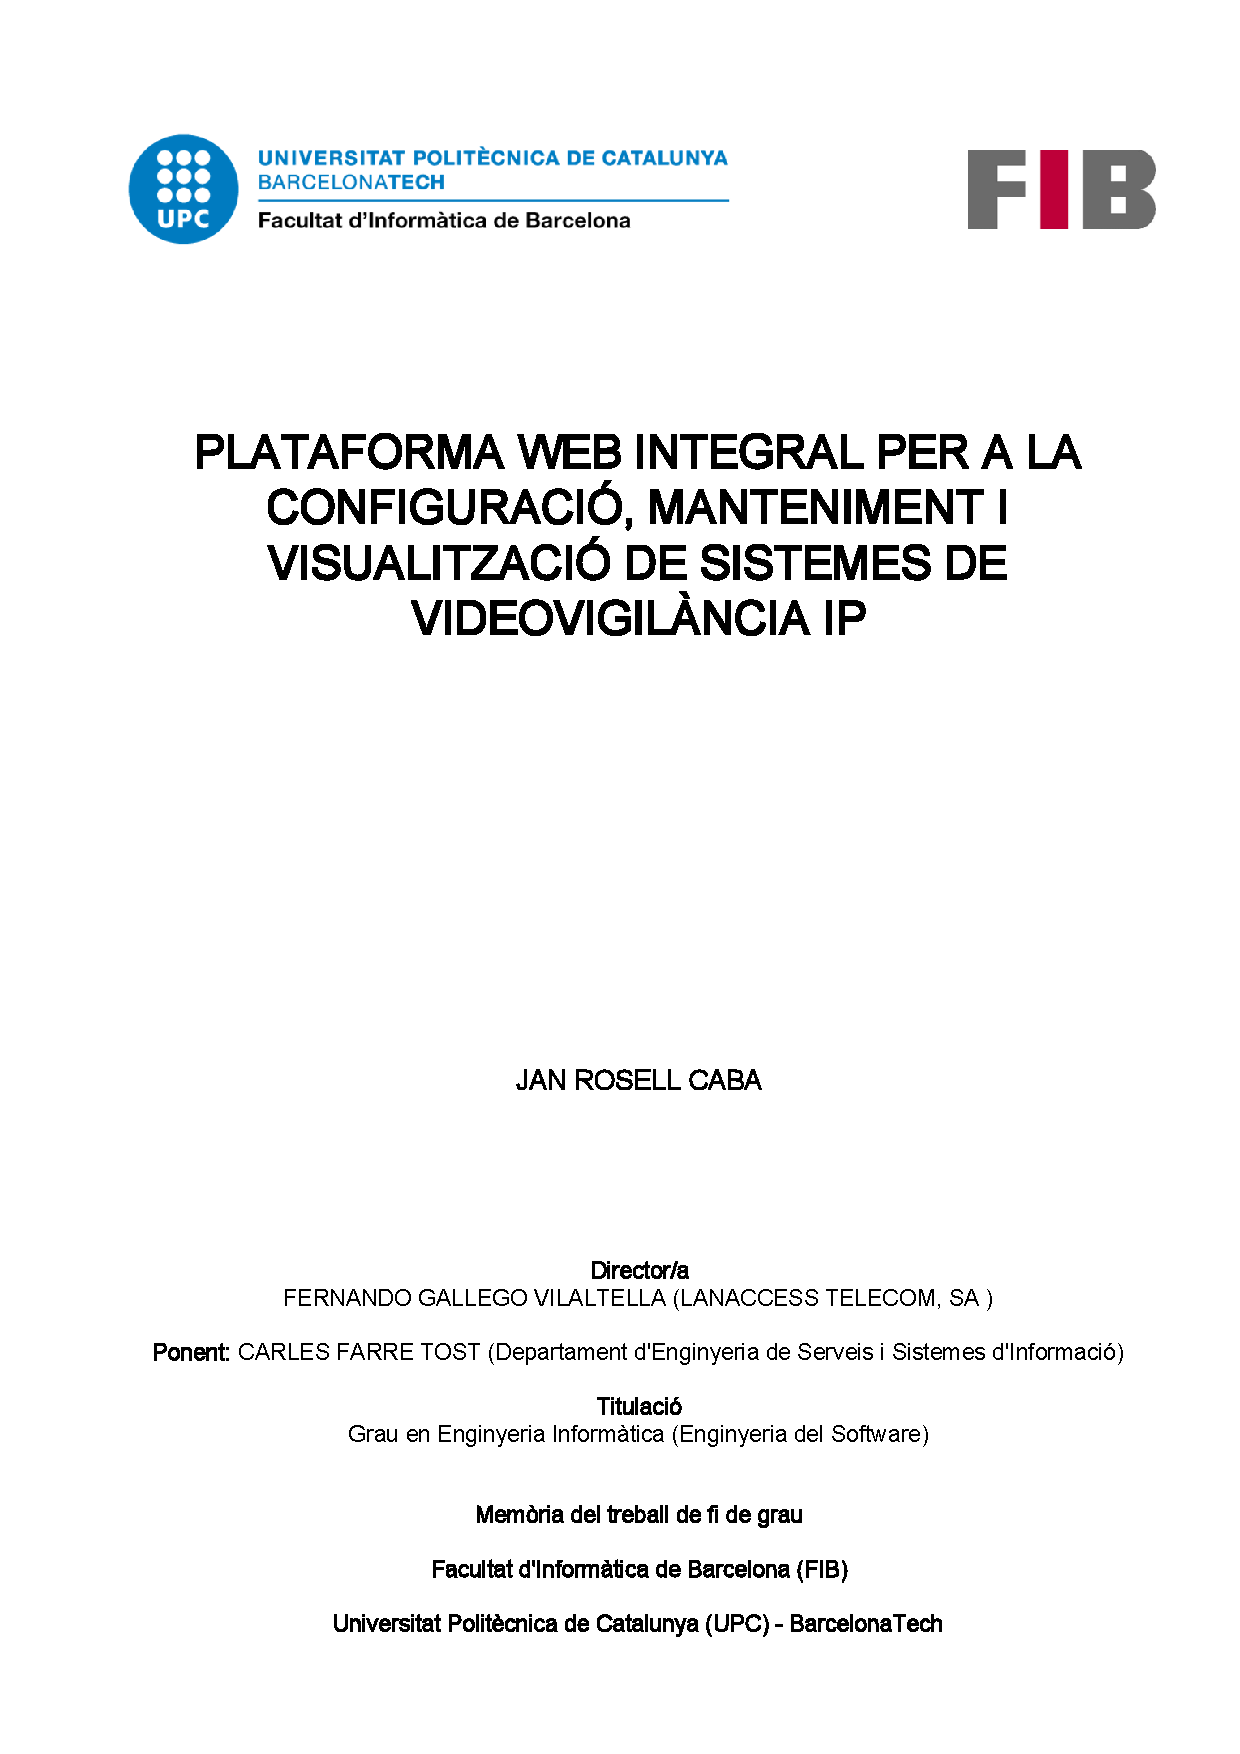
\includepdf{portada.pdf}

\pagenumbering{roman}
\chapter*{Resum}
Aquest treball presenta el disseny i la implementació de \textbf{Web Core View}, una interfície web d'administració \textit{embedded} per a la nova generació de videogravadors NXT de Lanaccess Telecom, SA. El projecte neix d'una doble necessitat: substituir la plataforma web de gestió \textit{legacy} dels anys 90, basada en controls \textbf{ActiveX} avui incompatibles amb els navegadors moderns, per una solució accessible i segura; i disposar d'una versió autònoma per a un únic videogravador, que s'executa directament al hardware del dispositiu, permetent a empreses petites gestionar-lo des de qualsevol navegador sense infraestructura centralitzada. La solució s'ha construït amb \textbf{Angular 19} i el nou paradigma de reactivitat basat en \textbf{Signals}, sobre una arquitectura de \textbf{microserveis coordinats}. Les dues aportacions tècniques principals són el motor de configuració dinàmic, que desacobla la interfície de l'evolució del \textit{firmware} mitjançant esquemes JSON enviats pel backend, i la integració de \textbf{WebRTC} per a la visualització de vídeo en directe amb latències baixes ($<$300~ms) sense necessitat de \textit{plugins}; la reproducció de gravacions es gestiona amb \textbf{HLS}. El sistema incorpora a més gestió d'alarmes en temps real, actualització de \textit{firmware} remota via fitxer \texttt{.bin} amb seguiment d'estat en directe, i una capa de seguretat que gestiona les sessions i garanteix la integritat de l'aplicació davant d'accessos simultanis. La interfície, dissenyada per a operadors de seguretat professionals, és reactiva i adaptativa, accessible des de tauletes de manteniment fins a monitors d'alta resolució.
\newpage
\chapter*{Abstract}
This work presents the design and implementation of \textbf{Web Core View}, an embedded web administration interface for the new generation of NXT video recorders at Lanaccess Telecom, SA. The project arises from a twofold need: to replace the legacy web management platform from the 1990s, based on \textbf{ActiveX} controls now incompatible with modern browsers, with an accessible and secure solution; and to provide a standalone version for a single video recorder, running directly on the device hardware, allowing small businesses to manage it from any browser without centralised infrastructure. The solution has been built with \textbf{Angular 19} and the new reactivity paradigm based on \textbf{Signals}, on top of a \textbf{coordinated microservices} architecture. The two main technical contributions are the dynamic configuration engine, which decouples the interface from firmware evolution through JSON schemas sent by the backend, and the integration of \textbf{WebRTC} for live video streaming with low latency ($<$300~ms) without the need for external plugins; recording playback is handled with \textbf{HLS}. The system also incorporates real-time alarm management, remote firmware updates via \texttt{.bin} file with live status tracking, and a security layer that manages user sessions and guarantees the integrity of the application against concurrent access. The interface, designed for professional security operators, is reactive and adaptive, accessible from maintenance tablets to high-resolution monitors.

\tableofcontents
\listoftables
\listoffigures

\newpage
\pagenumbering{arabic}

\chapter{Introducció i Context}
\label{ch:introduccio}

En aquest primer capítol es defineix el marc en el qual es desenvolupa el projecte, s'analitza la problemàtica de la plataforma web \textit{legacy} de l'empresa Lanaccess i es justifica la necessitat de substituir-la per una solució moderna. Així mateix, es detallen els objectius, l'abast i els actors implicats en el cicle de vida del software.

\section{Context del projecte}
Aquest Treball de Final de Grau (TFG) consisteix en el disseny i desenvolupament de \textbf{Web Core View}, una aplicació web moderna destinada a la gestió centralitzada dels videogravadors (\textit{Network Video Recorder}, d'ara endavant \textbf{NVR}) de la família \textbf{NXT} de l'empresa Lanaccess Telecom, SA. El projecte es realitza en col·laboració amb aquesta empresa tecnològica, especialitzada en el desenvolupament de solucions professionals de videovigilància i seguretat electrònica.

El treball s'emmarca dins de la \textbf{Modalitat B} del TFG i de l'especialitat d'Enginyeria de Software, posant èmfasi en arquitectures \textit{frontend} i \textit{backend} modernes, seguretat en la comunicació i integració de protocols. L'objectiu és modernitzar la plataforma tecnològica de l'empresa, substituint l'aplicació web \textit{legacy} construïda als anys 90 amb tecnologies avui obsoletes (\textbf{ActiveX}) per una interfície de control i administració \textit{embedded} que s'executa directament al propi videogravador NXT, basada en l'ecosistema Angular i protocols estàndard oberts (WebRTC, HLS, WSS).

\section{Identificació del problema i motivació}
La plataforma \textit{legacy} de Lanaccess és una aplicació web construïda als anys 90 que depenia en la seva totalitat dels controls \textbf{ActiveX} de Microsoft per a la visualització de vídeo i la interacció amb el maquinari. Amb la retirada oficial del suport a Internet Explorer 11 per part de Microsoft el juny del 2022 \cite{microsoft_ie11_eol}, l'últim navegador capaç d'executar controls ActiveX va quedar obsolet, fent la plataforma pràcticament inoperativa per a qualsevol instal·lació moderna. Aquesta obsolescència es concreta en tres problemes fonamentals:

\begin{itemize}
  \item \textbf{Incompatibilitat amb navegadors moderns:} ActiveX és una tecnologia exclusiva d'Internet Explorer. Els navegadors actuals (Chrome, Firefox, Edge, Safari) han eliminat completament el suport per a \textit{plugins} propietaris externs per raons de seguretat, de manera que la plataforma \textit{legacy} és avui inaccessible des de qualsevol navegador d'ús estàndard.
  \item \textbf{Rigidesa davant hardware heterogeni:} La interfície estàtica de la plataforma \textit{legacy} no pot adaptar-se a la disparitat de paràmetres i \textit{firmwares} dels videogravadors NXT (adreces IP, ports, lògiques d'alarma, còdecs suportats). Qualsevol canvi en el maquinari suportat requereix modificar i redistribuir manualment el codi de l'aplicació.
  \item \textbf{Absència de capacitats en temps real:} La interfície, basada en pàgines estàtiques dels anys 90 (recàrregues completes, sense comunicació asíncrona), no ofereix cap de les funcionalitats de temps real que requereixen els operadors de seguretat actuals: visualització de vídeo en directe, alertes instantànies ni configuració dinàmica.
\end{itemize}

Paral·lelament, Lanaccess ha identificat una \textbf{necessitat de mercat addicional}: oferir una solució de gestió autònoma orientada a \textbf{empreses petites} amb un únic videogravador NXT. El model anterior era una aplicació web centralitzada, allotjada en un servidor intern de la instal·lació, que gestionava simultàniament tot el parc de dispositius d'una gran infraestructura. Aquesta arquitectura resulta sobredimensionada i innecessàriament complexa per a clients amb una sola unitat de gravació. Així, \textit{Web Core View} neix amb una doble finalitat: modernitzar la plataforma tecnològica obsoleta i, alhora, proporcionar una solució \textit{embedded} lleugera que s'executi directament en el propi videogravador NXT, permetent la gestió autònoma de l'equip des de qualsevol navegador sense requerir infraestructura centralitzada addicional.

\section{Estat de l'art i alternatives existents}

\subsection{Estat de l'art}
El mercat de la videovigilància IP és un dels sectors tecnològics de major creixement, en el qual fabricants com Hikvision i Dahua han assolit una posició de lideratge gràcies a dispositius d'alt rendiment i cost competitiu \cite{ihs_video_surveillance}. Les seves solucions incorporen interfícies web integrades als videogravadors, però sovint requereixen la instal·lació de \textit{plugins} propietaris per a la visualització de vídeo, fet que limita la seva compatibilitat a navegadors específics i planteja riscos de seguretat corporativa.

Aquesta limitació reflecteix una tendència de canvi estructural del sector cap al \textbf{vídeo \textit{plugin-free}}. L'aparició d'estàndards oberts com \textbf{WebRTC} \cite{rfc8825} i \textbf{HLS} \cite{hls_apple} ha suposat un punt d'inflexió: permeten la transmissió de fluxos multimèdia de baixa latència i la reproducció d'enregistraments de forma nativa al navegador, sense extensions externes. Paral·lelament, la gran majoria d'organitzacions bloquegen per política interna la instal·lació de \textit{plugins} a les estacions de treball dels operadors per evitar vectors d'atac, fet que converteix el \textit{plugin-free} en un requisit de compliment de seguretat corporativa per a grans infraestructures.

D'altra banda, les plataformes VMS (\textit{Video Management System}) de gamma alta, com Milestone XProtect \cite{milestone_xprotect} o Genetec Security Center \cite{genetec_security_center}, ofereixen solucions modulars i molt potents, però requereixen una infraestructura de servidors dedicada, costos de llicenciament per canal elevats i personal TI especialitzat. Estan orientades a grans instal·lacions corporatives i no contemplen un model de desplegament autònom en un únic NVR sense servidors addicionals.

\subsection{Taula comparativa}
La Taula~\ref{tab:comparativa_mercat} compara les dues categories de solucions de mercat predominants, la plataforma \textit{legacy} i la proposta de Web Core View, diferenciant entre fabricants de maquinari (Hikvision/Dahua) i plataformes VMS d'empresa (Milestone/Genetec).

\begin{table}[h!]
  \centering
  \caption{Comparativa de solucions de videovigilància web.}
  \label{tab:comparativa_mercat}
  \resizebox{\textwidth}{!}{
    \begin{tabular}{@{}lllll@{}}
      \toprule
      \textbf{Característica} & \textbf{Web Legacy (ActiveX)} & \textbf{Hikvision / Dahua} & \textbf{VMS (Milestone / Genetec)} & \textbf{Web Core View} \\ \midrule
      Accés web          & IE / ActiveX (obsolet)  & Parcial (\textit{plugins}) & App dedicada / client ric     & \textbf{Navegador modern}              \\
      Protocol de vídeo  & RTSP via ActiveX        & RTSP / H.264               & RTSP / RTMP                   & \textbf{WebRTC / HLS}                  \\
      Configuració       & Estàtica                & Fixa per model             & Propietària                   & \textbf{Dinàmica (\textit{Schema-driven})} \\
      Cost / llicències  & N/A (intern)            & Inclòs en hardware         & Alt (per canal/càmera)        & \textbf{Inclòs al NXT}                 \\
      Desplegament       & Servidor centralitzat   & Servidor centralitzat      & Servidors dedicats            & \textbf{Autònom (\textit{embedded})}   \\ \bottomrule
    \end{tabular}
  }
  \par\smallskip
  \small Font: Elaboració pròpia a partir de la documentació pública dels fabricants \cite{milestone_xprotect, genetec_security_center}.
\end{table}

\section{Anàlisi d'alternatives i justificació de la solució}
Per garantir l'èxit i la sostenibilitat del projecte, s'han avaluat diferents camins tecnològics per als pilars fonamentals de programari, vídeo, concurrència i em\-ma\-gat\-ze\-mat\-ge del sistema:

\subsection{Alternativa de Framework Frontend: Angular 19 vs. React / Vue}
\begin{itemize}
  \item \textbf{React / Vue:} Són llibreries extremadament populars i flexibles, usades en entorns tan exigents com la banca o l'administració pública. En ser arquitectures no opinades, requereixen integrar múltiples llibreries de tercers (ruteig, formularis, \textit{state management}) per cobrir funcionalitats que en un \textit{framework} empresarial ja venen integrades, cosa que implica un cost de manteniment i auditoria de dependències superior en un projecte de vida llarga.
  \item \textbf{Angular 19:} És un \textit{framework} empresarial complet: proporciona ruteig, formularis reactius, injecció de dependències i un sistema de mòduls propi. Escrit nativament en TypeScript, incorpora eines de \textit{testing} integrades (Jasmine/Karma) i una estructura opinada que facilita la consistència del codi en equips.
  \item \textbf{Justificació:} S'ha escollit \textbf{Angular 19} per la seva estructura opinada que redueix decisions arquitecturals arbitràries, el tipatge estàtic de TypeScript, el motor de formularis reactius nadiu, les eines de \textit{testing} integrades i, principalment, la introducció de les \textbf{Signals} \cite{angular_signals} com a mecanisme natiu i eficient de gestió de l'estat reactiu, que permet prescindir de \textit{Zone.js} i optimitza el rendiment en dispositius \textit{embedded}.
\end{itemize}

\subsection{Alternativa de vídeo: Arquitectura Híbrida WebRTC i HLS vs. RTSP / RTMP}
\begin{itemize}
  \item \textbf{RTSP (Real-Time Streaming Protocol):} És el protocol de facto utilitzat internament per les càmeres IP i sistemes VMS clàssics. No obstant això, és completament incompatible de forma nativa amb els navegadors web actuals, obligant a utilitzar transcodificadors molt costosos o \textit{plugins} externs propietaris en desús.
  \item \textbf{RTMP (Real-Time Messaging Protocol):} Protocol clàssic molt lligat a la tecnologia ja obsoleta d'Adobe Flash, actualment completament desapareguda de l'ecosistema web estàndard.
  \item \textbf{WebRTC i HLS:} Són els dos únics estàndards web moderns reconeguts pel W3C que permeten la reproducció de vídeo nativa (HTML5) de forma segura i sense cap mena d'extensió o control extern.
  \item \textbf{Justificació:} S'ha optat per una \textbf{arquitectura híbrida complementària} que explota el millor de cada protocol en lloc de triar-ne només un:
        \begin{enumerate}
          \item \textbf{WebRTC:} S'utilitza principalment per al \textbf{vídeo en directe}, on la latència ultra-baixa ($<300$~ms) i el transport sobre UDP sota xifratge DTLS són indispensables per vigilar o respondre a amenaces immediates.
          \item \textbf{HLS (HTTP Live Streaming) \cite{hls_apple}:} S'utilitza per a la \textbf{reproducció de gravacions històriques}, on la ultra-baixa latència no és prioritària però es requereix un control molt precís de descàrrega per blocs (segments), commutació dinàmica de qualitat i la capacitat de fer desplaçaments lliures (\textit{seek}) sobre l'històric mitjançant TCP. També actua com a \textit{fallback} per al vídeo en directe si els tallafocs bloquegen el trànsit WebRTC.
        \end{enumerate}
\end{itemize}

\subsection{Alternativa de Base de Dades per a Alarmes: SQLite3 vs. PostgreSQL / MongoDB}
\begin{itemize}
  \item \textbf{PostgreSQL / MySQL:} Són bases de dades relacionals molt potents, però funcionen com a serveis de sistema independents. Requereixen un consum elevat i constant de memòria RAM i CPU per mantenir el dimoni actiu, sent una sobrecàrrega inacceptable en dispositius embedded limitats.
  \item \textbf{MongoDB:} Base de dades documental NoSQL ideal per a grans volums de dades desestructurades, però amb una pila tecnològica pesada i requisits de recursos inassequibles per al maquinari de gravació local.
  \item \textbf{SQLite3:} És un motor de base de dades relacional \textit{serverless}, transaccional (ACID) i auto-tingut que s'executa en el mateix procés del backend (in-process). Guarda tota la informació en un únic fitxer físic al disc.
  \item \textbf{Justificació:} S'ha seleccionat \textbf{SQLite3} com el motor de base de dades per al registre d'alarmes i logs del dispositiu, atès que ofereix un rendiment excel·lent per a lectures i escriptures ràpides amb un consum residual de memòria ($<15$~MB), essent ideal per als gravadors NXT de Lanaccess amb recursos de memòria i CPU limitats.
\end{itemize}

\subsection{Alternativa de Còdec de Vídeo: H.264 i H.265 coexistents}
\begin{itemize}
  \item \textbf{H.264 (AVC):} Còdec universal amb descodificació hardware garantida en el 100\% dels navegadors i dispositius. Consum d'ample de banda i d'espai de disc superior per a la mateixa qualitat d'imatge.
  \item \textbf{H.265 (HEVC):} Redueix fins a la meitat l'espai d'emmagatzematge i l'ample de banda per a la mateixa qualitat, però el seu suport web depèn de la disponibilitat de descodificació hardware al terminal client, degut a restriccions de patents.
  \item \textbf{Justificació:} S'ha optat per una \textbf{estratègia dinàmica de coexistència}: el sistema prioritza H.265 quan la càmera i el terminal client ho suporten (màxim estalvi de disc), i commuta automàticament a H.264 en cas contrari (portabilitat universal). Els detalls de la detecció de capacitats i la lògica de commutació s'expliquen al Capítol~\ref{ch:implementacio}.
\end{itemize}

\subsection{Alternativa de configuració: Estàtica vs. Schema-driven}
\begin{itemize}
  \item \textbf{Formularis estàtics:} Programar una pantalla per a cada menú de configuració és més ràpid a curt termini però genera un deute tècnic insostenible: cada canvi en el \textit{firmware} del videogravador NXT —un nou paràmetre, un rang vàlid diferent, un camp eliminat— obligaria a actualitzar i redistribuir el \textit{frontend}. En una plataforma amb múltiples models de hardware i \textit{firmwares} en evolució continuada, això és inviable.
  \item \textbf{Motor Schema-driven:} El \textit{backend} envia al \textit{frontend} un diccionari pla de claus en notació de punts (p. ex., \texttt{camera.\{id\}.stream.codec}) on cada valor porta metadades amb prefix \textit{underscore}: \texttt{\_type}, \texttt{\_allowedValues}, \texttt{\_min}, \texttt{\_max}, \texttt{\_default} i \texttt{\_description}. El \textit{frontend} actua com un intèrpret universal que renderitza automàticament el control adequat —selector, camp numèric, \textit{toggle}, etc.— sense conèixer el model concret de videogravador ni la versió de \textit{firmware}.
  \item \textbf{Justificació:} S'ha optat per la solució \textbf{Schema-driven} perquè és la característica diferenciadora del projecte: permet que \textbf{Web Core View} sigui compatible amb qualsevol model futur de la família NXT de Lanaccess sense modificar ni una línia de codi del \textit{frontend}. El format real del \textit{schema} s'explica en detall a l'Annex~A.1 de la memòria.
\end{itemize}

\subsection{Alternativa de gestió d'estat: NgRx vs. Angular Signals}
\begin{itemize}
  \item \textbf{NgRx:} Implementació del patró Redux per a l'ecosistema Angular, robusta per a aplicacions gegantines amb estats complexos compartits entre mòduls. Implica un \textit{boilerplate} elevat (accions, \textit{reducers}, efectes, selectors) i un cost d'aprenentatge notable.
  \item \textbf{Angular Signals:} La nova eina nativa d'Angular 19 per a la gestió de la reactivitat granular \cite{angular_signals}. Permet que els components reaccionin exactament als canvis d'estat que els afecten, sense necessitat de \textit{Zone.js}.
  \item \textbf{Justificació:} S'ha seleccionat \textbf{Signals} per la seva lleugeresa i eficiència en el renderitzat. En un entorn \textit{embedded} on la CPU s'ha de prioritzar per al vídeo, la reactivitat nativa de Signals permet prescindir de les comprovacions constants de \textit{Zone.js}, optimitzant el rendiment global del sistema.
\end{itemize}

\subsection{Alternativa de mecanisme de sessió: JWT vs. Cookies HttpOnly/Secure}
\begin{itemize}
  \item \textbf{JWT (\textit{JSON Web Token}):} Mecanisme d'autenticació sense estat (\textit{stateless}) \cite{rfc7519} que codifica les credencials al propi \textit{token} signat. La gestió des del \textit{frontend} implica emmagatzemar el \textit{token} a \textit{LocalStorage} o \textit{SessionStorage}, fet que els exposa a atacs XSS (\textit{Cross-Site Scripting}) si hi ha una injecció de codi maliciós.
  \item \textbf{Cookies \texttt{HttpOnly}/\texttt{Secure}:} La \textit{cookie} de sessió és gestionada exclusivament per NGINX: s'estableix al \textit{backend}, s'envia al navegador amb els atributs \texttt{HttpOnly} i \texttt{Secure}, i el JavaScript de l'aplicació no en té accés en cap moment. L'estat de sessió es manté en un Signal privat en memòria al \textit{frontend} (zero-persistència: un F5 equival a tancar sessió).
  \item \textbf{Justificació:} S'ha optat per les \textbf{cookies \texttt{HttpOnly}/\texttt{Secure}} gestionades per NGINX perquè eliminen el vector d'atac XSS sobre les credencials: cap \textit{script} del navegador no pot llegir ni exfiltrar la \textit{cookie}. Aquesta decisió s'alinea amb les recomanacions de seguretat de l'OWASP per a aplicacions en entorns de control d'accés físic.
\end{itemize}

\subsection{Alternativa de notificacions en temps real: WebSockets vs. SSE vs. Long Polling}
\begin{itemize}
  \item \textbf{Long Polling:} El client fa peticions HTTP repetides fins que el servidor disposa de dades noves. Solució senzilla però ineficient: genera múltiples connexions curtes i latències variables, inadequada per a notificacions d'alarmes crítiques.
  \item \textbf{SSE (\textit{Server-Sent Events}):} Connexió HTTP unidireccional (servidor $\rightarrow$ client), lleugera i nativa al navegador. Adequada per a \textit{feeds} de dades en un sol sentit, però no permet enviar comandes del client al servidor per la mateixa connexió.
  \item \textbf{WebSockets (WSS):} Connexió TCP persistent i bidireccional \cite{rfc6455} que permet tant rebre notificacions \textit{push} del servidor com enviar comandes del client (p. ex., marcar una alarma com a llegida) amb latència mínima.
  \item \textbf{Justificació:} S'ha escollit \textbf{WebSockets} per la seva naturalesa bidireccional, necessària per als dos canals del sistema: el canal global de notificacions (\texttt{/ws/la-core-no\-ti\-fier/}) i el canal d'alarmes (\texttt{/ws/la-core-alarm/}), que requereix tant rebre alertes com confirmar-ne la lectura des del client.
\end{itemize}

\subsection{Alternativa de proxy invers: NGINX vs. accés directe als microserveis}
\begin{itemize}
  \item \textbf{Accés directe als microserveis:} Exposar cada microservei del \textit{backend} en ports independents obliga el navegador a realitzar peticions \textit{cross-origin}, fent necessaris encapçalaments CORS complexos i impedint l'ús de cookies \texttt{HttpOnly} (que no es transmeten en peticions \textit{cross-origin} per defecte).
  \item \textbf{NGINX com a proxy invers:} Centralitza tots els microserveis sota un únic origen (\textit{same-origin}), enrutant per prefix de ruta. Gestiona el cicle de vida de les \textit{cookies} de sessió de forma transparent i actua com a punt únic de control de seguretat (TLS, capçaleres HTTP de seguretat).
  \item \textbf{Justificació:} S'ha escollit \textbf{NGINX} \cite{nginx_admin} per la seva maduresa i rendiment en sistemes Linux embeguts: permet centralitzar la seguretat, implementar les \textit{cookies} \texttt{HttpOnly}/\texttt{Secure} de forma consistent sense modificar cap microservei del \textit{backend}, i elimina el problema CORS de manera estructural.
\end{itemize}

\section{Solució proposada i valor afegit}
\textbf{Web Core View} es proposa com una solució integral que aprofita les noves funcionalitats de rendiment d'\textbf{Angular 19}. L'elecció d'aquesta versió respon a la voluntat d'utilitzar tecnologies actualitzades i de llarg suport. Les aportacions clau de la solució proposada són:
\begin{itemize}
  \item \textbf{Arquitectura Schema-driven:} La interfície interpreta un esquema JSON enviat pel gravador i genera automàticament els controls de configuració, assegurant compatibilitat amb qualsevol versió de hardware.
  \item \textbf{Gestió d'estat amb Signals:} L'ús d'\textbf{Angular Signals} representa un canvi de paradigma en la reactivitat. Aquesta funcionalitat permet una gestió granular dels canvis, optimitzant el rendiment del \textit{frontend} i garantint una fluïdesa absoluta fins i tot amb múltiples fluxos de vídeo simultanis, evitant sobrecàrregues de CPU innecessàries al terminal del client.
  \item \textbf{Control de concurrència:} Implementació d'un servei de bloqueig en temps real per evitar conflictes d'edició entre administradors.
  \item \textbf{Arquitectura d'esdeveniments:} Ús de \textit{WebSockets} (WSS) per rebre notificacions d'alarmes, notificacions del sistema i errors de forma immediata.
  \item \textbf{Desplegament autònom (single-NVR):} L'aplicació s'executa directament dins del propi videogravador NXT com a servidor web \textit{embedded}. Això permet que empreses petites amb un únic dispositiu puguin gestionar-lo de forma completa i autònoma des de qualsevol navegador, sense necessitat d'infraestructura centralitzada addicional ni de programari extern. Aquesta capacitat obre un nou segment de mercat per a Lanaccess que la plataforma \textit{legacy} anterior no podia cobrir.
\end{itemize}

\section{Objectius del projecte}
\subsection{Objectiu general}
Dissenyar i desenvolupar una consola de gestió web modular, reactiva i d'alt rendiment que centralitzi la gestió tècnica i operativa dels NVRs NXT de Lanaccess, substituint la plataforma web \textit{legacy} dels anys 90 i les seves tecnologies obsoletes (ActiveX) per una arquitectura i interfície completament modernes.

\subsection{Objectius específics}
\begin{itemize}
  \item Desenvolupar un motor de configuració dinàmic basat en esquemes metadada.
  \item Integrar un mòdul de visualització híbrid compatible amb WebRTC i HLS (H264/H265).
  \item Implementar la gestió d'alarmes en temps real mitjançant comunicació bidireccional.
  \item Facilitar el manteniment remot (\textit{firmware}, llicències i logs) via navegador.
  \item Dissenyar l'aplicació com una solució autònoma \textit{embedded} capaç de funcionar directament en un únic NVR NXT (\textit{single-NVR}), sense dependència de servidors centralitzats, per cobrir el segment d'empreses petites.
\end{itemize}

\section{Abast i Obstacles}
\subsection{Abast funcional}
L'aplicació ha d'oferir un cicle complet de gestió: des de l'autenticació segura de l'usuari fins a la monitorització de càmeres en directe, la cerca de gravacions històriques i la configuració avançada de xarxa i paràmetres de sistema. El disseny ha de contemplar el desplegament autònom en un únic videogravador NXT (mode \textit{single-NVR}) com a cas d'ús principal, garantint que tota la funcionalitat sigui operable sense infraestructura externa.

\subsection{Obstacles detectats}
S'han identificat reptes tècnics que afecten diferents actors:
\begin{itemize}
  \item \textbf{Complexitat del vídeo natiu:} El repte de visualitzar H.265 sense \textit{plugins}. Afecta al \textbf{Projectista} (recerca de llibreries) i a l'\textbf{Usuari final} (potencial latència).
  \item \textbf{Sincronització en temps real:} Requereix una gestió d'estat robusta perquè l'\textbf{Operador} vegi alarmes sense retard.
  \item \textbf{Seguretat i NGINX:} Configuració del \textbf{Proxy Invers} per centralitzar els microserveis sota un mateix origen i garantir polítiques de \textit{Same-Origin}.
\end{itemize}

\section{Actors implicats (Stakeholders)}
\begin{enumerate}
  \item \textbf{Usuari final (Operador):} Monitoritza càmeres i gestiona incidents.
  \item \textbf{Administrador tècnic:} Configura el sistema i realitza manteniment.
  \item \textbf{Lanaccess Telecom:} Proporciona el \textit{hardware} i coneixement de negoci.
  \item \textbf{Projectista (Estudiant):} Responsable únic de l'anàlisi i la implementació.
  \item \textbf{Equip docent (Director i Ponent):} Supervisen el rigor acadèmic i tècnic.
\end{enumerate}
\chapter{Gestió del projecte}
\label{ch:gestio}

En aquest capítol es descriu el marc metodològic utilitzat per al desenvolupament del projecte, la planificació temporal detallada de les tasques i l'anàlisi econòmica i de sostenibilitat del sistema.

\section{Metodologia i eines de treball}
El projecte es desenvolupa en un entorn professional dins de l’equip d’\textit{Embedded} de Lanaccess. S’ha optat per una \textbf{metodologia àgil basada en Kanban}, utilitzant l'eina \textit{Businessmap} per a la gestió visual del flux de treball. Aquesta elecció permet una gran flexibilitat i una resposta ràpida davant de canvis en els requeriments tècnics.

Els pilars del seguiment del projecte són:
\begin{itemize}
    \item \textbf{Reunions de sincronització (Daily):} Sessions diàries per coordinar el progrés, identificar bloquejos i alinear el \textit{frontend} amb l'estat del \textit{firmware}.
    \item \textbf{Seguiment acadèmic i professional:} El director del TFG supervisa l'evolució tècnica diàriament, mentre que es manté una comunicació constant amb el tutor de la universitat per garantir el rigor acadèmic.
    \item \textbf{Gestió de tasques:} Control del cicle de vida de cada funcionalitat des de la columna \textit{To Do} fins a \textit{Done}.
\end{itemize}

Respecte a l'enginyeria de software, se segueixen els estàndards següents:
\begin{itemize}
    \item \textbf{Control de versions:} Ús de \textbf{Git} amb el model \textbf{GitFlow} (branques \textit{master}, \textit{develop} i \textit{feature}). El repositori es troba allotjat en un GitLab local.
    \item \textbf{Stack tecnològic:} Angular 19 (Signals i Standalone Components) per al \textit{frontend} i implementacions en C++ 22 per a la comunicació de baix nivell en el \textit{backend}.
    \item \textbf{Qualitat:} Aplicació de principis SOLID i arquitectura modular.
\end{itemize}

\section{Planificació temporal}

\subsection{Descripció de les fases i tasques}
El projecte s'estructura en sis fases lògiques pactades amb l'empresa:

\begin{enumerate}
    \item \textbf{Gestió i Formació (GF):} Inclou l'autoformació en Angular 19 i la gestió administrativa de l'assignatura GEP.
    \item \textbf{Mòdul d'Autenticació i Core (AC):} Desenvolupament del \textit{login}, la \textit{home page} i el sistema base de \textit{logs} i alertes.
    \item \textbf{Manteniment i Configuració Base (MC):} Gestió de llicències, actualització de \textit{firmware} i integració del motor de base de dades.
    \item \textbf{Alarmes i Sistema de Vídeo Directe (AV):} Implementació del motor d'alarmes via WSS i visualització en temps real.
    \item \textbf{Mòdul de Gravacions i Configuració Avançada (GV):} Reproducció d'històrics (HLS) i motor de configuració dinàmica \textit{Schema-driven}.
    \item \textbf{Finalització i Memòria (FM):} Fase de correcció d'errors, repàs de qualitat i redacció final.
\end{enumerate}

\subsection{Recursos identificats}
Per a l'execució del projecte es requereixen els següents recursos:
\begin{itemize}
    \item \textbf{Humans (Rols):} Cap de Projecte (planificació), Analista (disseny d'arquitectura), Programador (codificació) i Tester (validació).
    \item \textbf{Materials:} Ordinador portàtil (ASUS Expertbook), videogravador Lanaccess de proves i espai de despatx equipat.
    \item \textbf{Software:} VS Code, Git, Angular 19, RxJS i llibreries de vídeo (WebRTC, HLS.js).
\end{itemize}

\subsection{Estimació d'hores i Diagrama de Gantt}
S'ha estimat una càrrega total de \textbf{540 hores} (18 ECTS). La Taula \ref{tab:estimacio_hores} resumeix el repartiment temporal segons el planning oficial.

\begin{table}[htbp]
\centering
\caption{Estimació d'hores i dependències de les tasques.}
\label{tab:estimacio_hores}
\small
\begin{tabular}{@{}llllc@{}}
\toprule
\textbf{ID} & \textbf{Tasca} & \textbf{Mes/Setmana} & \textbf{Dependència} & \textbf{Hores} \\ \midrule
GF1 & Formació Angular 19 & Desembre & - & 40 \\
AC1 & Login & Gener S1 & GF1 & 20 \\
AC2 & Home Page & Gener S2 & AC1 & 20 \\
AV1 & Core Alarm (WSS) & Feb S4 - Mar S1 & AC3 & 50 \\
AV3 & Càmeres Directe & Març S3 - S4 & AC2 & 50 \\
GV2 & System Config Avançat & Abr S3 - Maig S1 & MC2 & 60 \\
FM2 & Memòria TFG & Transversal & - & 80 \\ \midrule
\textbf{TOTAL} & & & & \textbf{540} \\ \bottomrule
\end{tabular}
\par\smallskip
\small Font: Elaboració pròpia.
\end{table}

\newpage
% --- AQUÍ POSES LA TEVA IMATGE DEL GANTT ---
\begin{figure}[htbp]
    \centering
    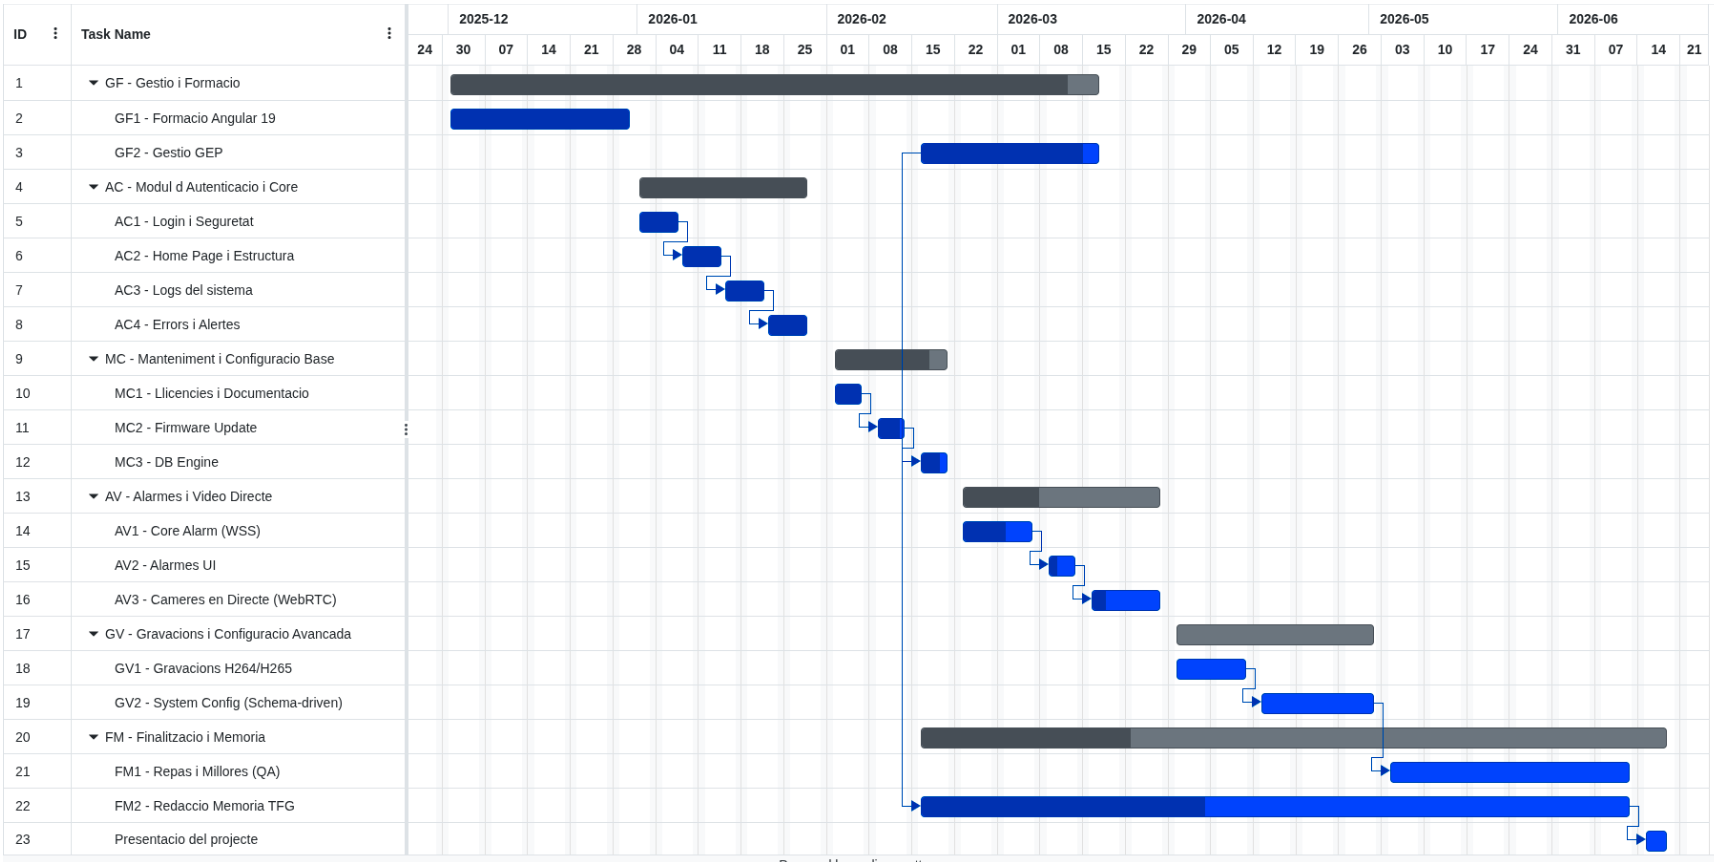
\includegraphics[width=1\textwidth]{figures/gantt.png}
    \caption{Diagrama de Gantt del projecte.}
    \label{fig:gantt}
    \small Font: Elaboració pròpia.
\end{figure}

\subsection{Gestió del risc i desviacions reals}
S'han previst plans de contingència per a retards en la formació o incompatibilitats en els protocols de vídeo (WebRTC). Actualment, s'han detectat desviacions en [completar amb la teva experiència real, ex: la implementació del motor WebRTC per problemes de latència].

\section{Anàlisi econòmica}
L'estimació econòmica s'ha realitzat assumint rols professionals i preus de mercat actuals, afegint un factor d'1,35 per cobrir la Seguretat Social.

\subsection{Costos de personal}
\begin{table}[htbp]
\centering
\caption{Costos de recursos humans per rol.}
\label{tab:costos_humans}
\begin{tabular}{@{}lcccc@{}}
\toprule
\textbf{Rol} & \textbf{Sou Brut/h (€)} & \textbf{Cost Real/h (€)} & \textbf{Hores} & \textbf{Total (€)} \\ \midrule
Project Manager & 25,00 & 33,75 & 90 & 3.037,50 \\
Analista & 20,00 & 27,00 & 100 & 2.700,00 \\
Programador & 18,00 & 24,30 & 250 & 6.075,00 \\
Tester & 13,00 & 17,55 & 100 & 1.755,00 \\ \midrule
\textbf{TOTAL CPA} & & & \textbf{540} & \textbf{13.567,50} \\ \bottomrule
\end{tabular}
\end{table}

\subsection{Costos totals i control de gestió}
Sumant l'amortització del hardware (210,00 €), els costos indirectes \- d'oficina (1.150,00 €) i un marge de contingència del 10 \%, el pressupost final estimat és de \textbf{16.810,40 €}.

El control de gestió es realitza mitjançant la fórmula de desviació de costos:
\[ \text{Desviació} = (\text{Hores Planificades} - \text{Hores Reals}) \times \text{Cost/h} \]

\section{Informe de sostenibilitat}
\begin{itemize}
    \item \textbf{Dimensió Econòmica:} La solució \textit{Schema-driven} permet adaptar el software a nous models de gravadors sense cost addicional, allargant la vida útil del producte.
    \item \textbf{Dimensió Ambiental:} L'ús de la plataforma web redueix els desplaçaments físics de tècnics a les instal·lacions del client, minimitzant la petjada de carboni.
    \item \textbf{Dimensió Social:} Millora la interfície de treball dels operadors de seguretat, reduint l'estrès operatiu en situacions d'incident crític.
\end{itemize}
\chapter{Especificació de Requisits}
\label{ch:requisits}

L'especificació de requisits constitueix la base fonamental del projecte \textit{Web Core View}. En tractar-se d'un sistema de gestió per a dispositius de seguretat crítica, la definició de les funcionalitats no només s'ha centrat en l'experiència d'usuari (UX), sinó també en la robustesa de la comunicació asíncrona i el desacoblament entre el maquinari i la interfície.

En aquest capítol es detallen els actors, les històries d'usuari mitjançant la metodologia \textit{Product Backlog}, i l'especificació detallada dels requisits funcionals i no funcionals.

\section{Metodologia d'extracció de requisits}
Els requisits aquí exposats s'han obtingut mitjançant un procés iteratiu amb l'equip d'Embedded de Lanaccess. S'han realitzat sessions d'anàlisi sobre l'aplicació web \textit{legacy} existent --- basada en tecnologies obsoletes com ActiveX --- i entrevistes amb tècnics de camp per identificar els ``punts crítics'' i les limitacions tecnològiques de la plataforma anterior.

\section{Identificació d'actors}
\label{sec:actors}
S'han definit tres actors principals, classificant-los segons el seu nivell d'interacció i privilegis dins del sistema:

\begin{description}
  \item[Administrador de Sistema:] Actor amb privilegis totals sobre el videogravador. El seu objectiu és la posada en marxa de l'equip i el manteniment correctiu. Les seves responsabilitats inclouen:
        \begin{itemize}
          \item Configuració de paràmetres de xarxa (IP, DNS, Gateways).
          \item Gestió del cicle de vida del hardware (Reinicis, actualització de firmware).
          \item Administració de comptes d'usuari i permisos.
        \end{itemize}

  \item[Operador:] Usuari final que utilitza la plataforma per a la monitorització.
        \begin{itemize}
          \item Visualització de vídeo en temps real (\textit{Live}).
          \item Visualització de gravacions històriques.
          \item Supervisió i silenciament d'alarmes en temps real.
        \end{itemize}

  \item[Videogravador (System Actor):] Malgrat ser un element de maquinari, en aquesta arquitectura actua com un usuari actiu que:
        \begin{itemize}
          \item Dicta l'estructura de la interfície mitjançant esquemes JSON.
          \item Notifica esdeveniments de forma proactiva via WebSockets.
          \item Gestiona el control de concurrència per evitar col·lisions de dades.
        \end{itemize}
\end{description}

\section{Històries d'Usuari (User Stories)}
S'utilitzen les \textit{User Stories} per definir el valor que cada funcionalitat aporta a l'usuari final. Cada història inclou els seus criteris d'acceptació.

\subsection{Mòdul de Visualització i Reproducció de Vídeo}
\begin{description}
  \item[\textbf{US-01: Streaming d'alta qualitat}] \hfill \\
        \textbf{Com a} Operador, \textbf{vull} veure el vídeo de qualsevol càmera connectada, \textbf{per tal de} vigilar l'espai protegit en temps real.
        \begin{itemize}
          \item \textit{Criteri 1:} La latència punta a punta ha de ser inferior a 300ms.
          \item \textit{Criteri 2:} El sistema ha de detectar automàticament si el navegador suporta WebRTC o ha de commutar a HLS.
        \end{itemize}

  \item[\textbf{US-02: Gestió de Mosaic}] \hfill \\
        \textbf{Com a} Operador, \textbf{vull} visualitzar fins a 4 càmeres simultàniament, \textbf{per tal de} tenir una visió global de la instal·lació.

  \item[\textbf{US-03: Consulta de gravacions històriques}] \hfill \\
        \textbf{Com a} Operador, \textbf{vull} consultar i reproduir el vídeo gravat del passat mitjançant una línia de temps (\textit{timeline}) gràfica, \textbf{per tal de} revisar incidents de seguretat que s'hagin produït prèviament.
        \begin{itemize}
          \item \textit{Criteri 1:} El reproductor ha de permetre saltar a qualsevol punt temporal passat amb una precisió de 1 segon a través del lliscador de la línia de temps.
          \item \textit{Criteri 2:} La reproducció de vídeo històric s'ha de transmetre mitjançant fragments HLS generats a petició pel gravador.
        \end{itemize}
\end{description}

\subsection{Mòdul de Configuració Dinàmica i Xarxa}
\begin{description}
  \item[\textbf{US-04: Configuració sense recàrrega de codi}] \hfill \\
        \textbf{Com a} Administrador, \textbf{vull} que els nous paràmetres afegits al firmware apareguin a la web sense haver de reprogramar el frontend.
        \begin{itemize}
          \item \textit{Criteri 1:} El frontend ha d'interpretar l'esquema JSON i renderitzar el component visual adequat de forma dinàmica (input, select, slider).
        \end{itemize}

  \item[\textbf{US-05: Configuració de xarxa i IP}] \hfill \\
        \textbf{Com a} Administrador, \textbf{vull} configurar els paràmetres de xarxa del dispositiu (adreça IP, màscara, ports), \textbf{per tal de} garantir la connectivitat del sistema.

  \item[\textbf{US-06: Gestió d'usuaris i permisos}] \hfill \\
        \textbf{Com a} Administrador, \textbf{vull} gestionar els perfils d'usuari i els seus permisos d'accés (grants), \textbf{per tal de} controlar quines accions i vistes pot utilitzar cadascú.
\end{description}

\subsection{Mòdul de Gestió d'Alarmes}
\begin{description}
  \item[\textbf{US-07: Recepció d'alarmes en temps real}] \hfill \\
        \textbf{Com a} Operador, \textbf{vull} rebre notificacions d'alarmes de forma immediata, \textbf{per tal d'}actuar ràpidament davant de qualsevol incidència de seguretat.
        \begin{itemize}
          \item \textit{Criteri 1:} L'alarma s'ha de mostrar a la interfície web en menys d'1 segon des de la seva detecció en el maquinari.
        \end{itemize}

  \item[\textbf{US-08: Configuració de regles d'alarma}] \hfill \\
        \textbf{Com a} Administrador, \textbf{vull} configurar i programar regles de detecció d'alarmes per a cada càmera, \textbf{per tal d'}automatitzar la detecció d'esdeveniments.
\end{description}

\subsection{Mòdul de Manteniment}
\begin{description}
  \item[\textbf{US-09: Consulta i renovació de llicència}] \hfill \\
        \textbf{Com a} Administrador de Sistema, \textbf{vull} consultar l'estat de la llicència del dispositiu i renovar-la quan sigui necessari, \textbf{per tal de} garantir la continuïtat del servei sense interrupcions.

  \item[\textbf{US-10: Actualització de firmware}] \hfill \\
        \textbf{Com a} Administrador de Sistema, \textbf{vull} actualitzar el firmware del dispositiu des de la interfície web, \textbf{per tal de} mantenir el sistema al dia amb les darreres millores i correccions de seguretat.

  \item[\textbf{US-11: Gestió de la configuració del sistema}] \hfill \\
        \textbf{Com a} Administrador, \textbf{vull} restaurar, carregar i descarregar la configuració del dispositiu, \textbf{per tal de} facilitar còpies de seguretat, migracions i recuperació davant de fallades.

  \item[\textbf{US-12: Accés a la documentació del sistema}] \hfill \\
        \textbf{Com a} Administrador de Sistema, \textbf{vull} tenir accés a tota la documentació tècnica del sistema des de la interfície web, \textbf{per tal de} resoldre dubtes i consultar especificacions sense necessitat de recursos externs.

  \item[\textbf{US-13: Descàrrega i consulta de logs}] \hfill \\
        \textbf{Com a} Administrador de Sistema, \textbf{vull} cercar i descarregar els registres d'esdeveniments del sistema, \textbf{per tal de} diagnosticar errors de funcionament o auditar l'ús de la plataforma.
\end{description}

\section{Requisits Funcionals (RF)}
A continuació es detallen els requisits tècnics dividits per blocs funcionals.

\subsection{RF-1: Gestió de l'Accés i Seguretat}
\begin{itemize}
  \item \textbf{RF-1.1 Autenticació:} El sistema ha de validar les credencials contra el servei \textit{Core Legacy}.
  \item \textbf{RF-1.2 Sessió Persistent:} Mantenir la sessió activa mitjançant un mecanisme de \textit{keep-alive} que refresqui la cookie de sessió cada 60 segons.
  \item \textbf{RF-1.3 Control de Concurrència:} El sistema ha de demanar un bloqueig d'escriptura quan un administrador entri en mode edició. Si un altre usuari intenta editar, el sistema mostrarà un avís de ``Només Lectura''.
\end{itemize}

\subsection{RF-2: Visualització Multimèdia}
\begin{itemize}
  \item \textbf{RF-2.1 Protocol WebRTC:} Implementació de la negociació SDP (\textit{Session Description Protocol}) per a vídeo en directe.
  \item \textbf{RF-2.2 Protocol HLS:} Generació de fragments de vídeo per a la reproducció de gravacions històriques i fallback de seguretat.
  \item \textbf{RF-2.3 Línia de Temps Històrica:} Interfície gràfica interactiva per a la cerca i consulta de gravacions passades amb selecció de franja horària.
\end{itemize}

\subsection{RF-3: Motor de Configuració Dinàmica}
Aquest és el requisit funcional més complex i innovador del sistema. El seu principi fonamental és el \textit{schema-driven design}: el gravador dicta l'estructura de la interfície mitjançant esquemes JSON, de manera que el frontend es desacobla completament de la lògica de baix nivell del maquinari.
\begin{itemize}
  \item \textbf{RF-3.1 Interpretació de l'Esquema:} El frontend ha de processar l'esquema JSON rebut del backend i renderitzar dinàmicament el component visual adequat per a cada paràmetre (camp de text, llista desplegable, \textit{slider} numèric). Les restriccions de tipus, rang i format (\textit{regex}) definides a l'esquema s'apliquen automàticament, sense requerir canvis al codi del frontend.
  \item \textbf{RF-3.2 Validació en temps real:} Qualsevol restricció declarada a l'esquema (\texttt{\_min}, \texttt{\_max}, \texttt{\_regex}, \texttt{\_allowedValues}) ha de ser compilada i validada pel motor del frontend abans d'enviar cap petició al backend.
\end{itemize}

\subsection{RF-4: Gestió d'Alarmes}
\begin{itemize}
  \item \textbf{RF-4.1 Recepció en temps real:} El sistema ha de rebre i mostrar les alarmes generades pel maquinari en menys d'1 segon mitjançant una connexió persistent amb el backend.
  \item \textbf{RF-4.2 Historial i filtrat:} El sistema ha de permetre consultar l'historial d'alarmes amb capacitat de filtrat per càmera, rang horari i estat (llegida / no llegida).
  \item \textbf{RF-4.3 Gestió de l'estat:} L'operador ha de poder marcar alarmes individuals com a llegides, arxivar-les o eliminar-les, i qualsevol d'aquestes accions ha de reflectir-se immediatament al backend.
  \item \textbf{RF-4.4 Configuració de regles:} L'administrador ha de poder definir i programar regles de detecció d'alarmes per a cada càmera connectada.
\end{itemize}

\subsection{RF-5: Manteniment i Administració del Sistema}
\begin{itemize}
  \item \textbf{RF-5.1 Registre d'activitat (Log):} El sistema ha de permetre cercar i descarregar els registres d'esdeveniments del dispositiu per facilitar el diagnòstic de fallades i l'auditoria d'ús.
  \item \textbf{RF-5.2 Actualització de firmware:} El sistema ha de gestionar el cicle complet d'actualització del firmware del gravador: pujada del binari, seguiment visual del progrés per fases i detecció automàtica de la tornada en línia del dispositiu un cop reiniciat.
  \item \textbf{RF-5.3 Gestió de la llicència:} El sistema ha de mostrar l'estat actual de la llicència del dispositiu (data de caducitat, funcionalitats habilitades) i permetre iniciar el procés de renovació.
  \item \textbf{RF-5.4 Gestió de la configuració general:} El sistema ha de permetre descarregar la configuració actual del dispositiu, carregar una configuració des d'un fitxer extern i restaurar els valors de fàbrica, amb confirmació explícita de l'usuari en operacions destructives.
  \item \textbf{RF-5.5 Accés a la documentació:} El sistema ha de proporcionar accés integrat a la documentació tècnica oficial del dispositiu (manuals, notes de versió, guies de configuració) sense necessitat de recórrer a recursos externs.
\end{itemize}

\subsection{RF-6: Gestió d'Usuaris i Permisos}
\begin{itemize}
  \item \textbf{RF-6.1 Administració de comptes:} L'administrador ha de poder crear, modificar i eliminar comptes d'usuari del sistema.
  \item \textbf{RF-6.2 Control d'accés basat en rols:} El sistema ha d'aplicar un model de permisos (\textit{grants}) que restringeixi l'accés a mòduls i operacions sensibles en funció del rol assignat a cada usuari.
  \item \textbf{RF-6.3 Canvi de credencials:} El sistema ha de permetre el canvi de contrasenya des de la pròpia interfície web, amb validació de la contrasenya actual.
\end{itemize}

\section{Requisits No Funcionals (RNF)}
Els RNF defineixen les qualitats del sistema i les restriccions tecnològiques.

\subsection{RNF-1: Rendiment i Eficiència}
\begin{itemize}
  \item \textbf{RNF-1.1 Utilització de CPU:} Atès que el videogravador té recursos limitats, s'ha optimitzat el trànsit per evitar el \textit{polling} innecessari, substituint-lo per una arquitectura basada en esdeveniments sobre dos canals WebSocket diferenciats: \textbf{la-core-notifier}, obert de forma persistent des del login per a notificacions globals del sistema, i \textbf{la-core-alarm}, actiu exclusivament a la pàgina d'alarmes per a esdeveniments de detecció en temps real.
  \item \textbf{RNF-1.2 Angular Signals:} La reactivitat de la interfície s'ha de basar en \textit{Angular Signals} per minimitzar les operacions de \textit{Zone.js} i evitar la renderització repetida innecessària del DOM, especialment crític amb vídeos actius.
\end{itemize}

\subsection{RNF-2: Robustesa i Disponibilitat}
\begin{itemize}
  \item \textbf{RNF-2.1 Tolerància a talls de xarxa:} El WebSocket ha d'intentar una reconnexió exponencial (re-try) en cas de pèrdua de connectivitat.
  \item \textbf{RNF-2.2 Fallback de Vídeo:} Si el port WebRTC (UDP 10000-20000) està bloquejat per firewall, el reproductor ha de commutar a HLS en menys de 5 segons.
  \item \textbf{RNF-2.3 Concurrència i Integritat:} Per garantir la consistència de les dades del sistema i evitar escriptures concurrents conflictives entre diferents usuaris administradors, s'exigeix un mecanisme de bloqueig pessimista (\textit{Pessimistic Locking}) en l'adquisició dels formularis de configuració activa. Cap usuari podrà modificar paràmetres del sistema si un altre usuari posseeix el \textit{lock} exclusiu d'aquell mòdul.
\end{itemize}

\subsection{RNF-3: Compatibilitat i Portabilitat}
\begin{itemize}
  \item \textbf{RNF-3.1 Multi-navegador:} Compatible amb les darreres dues versions de Google Chrome, Mozilla Firefox i Microsoft Edge.
  \item \textbf{RNF-3.2 Responsive Design:} La interfície ha de ser plenament operativa en resolucions des de 1024px d'amplada (tauletes de manteniment) fins a 4K (centres de control).
\end{itemize}

\section{Casos d'Ús detallats}
Per aprofundir en la funcionalitat del sistema, es presenta el diagrama de casos d'ús general (Figura \ref{fig:diagrama_casos_us}) i l'especificació detallada dels fluxos crítics.

\begin{figure}[htbp]
  \centering
  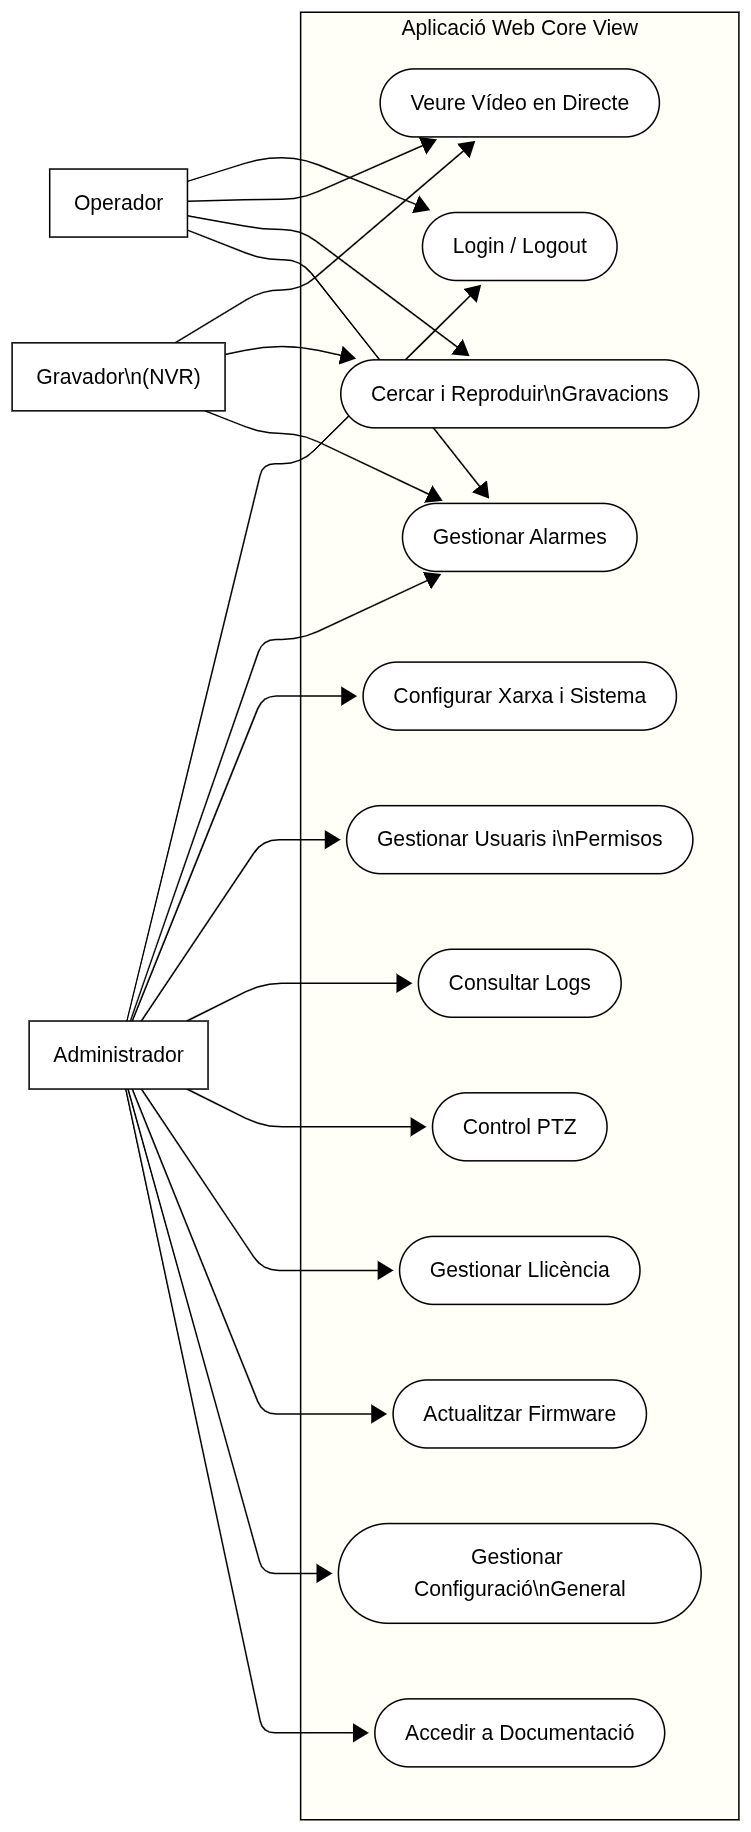
\includegraphics[width=0.9\textwidth, height=0.85\textheight, keepaspectratio]{figures/diagrames/use_cases.png}
  \caption{Diagrama UML de Casos d'Ús.}
  \label{fig:diagrama_casos_us}
  \small Font: Elaboració pròpia.
\end{figure}

\clearpage
\subsection{UC-00: Autenticació i inici de sessió}
L'autenticació és el flux d'entrada obligatori i prerequisit de tots els casos d'ús del sistema.

\begin{table}[htbp]
  \centering
  \small
  \begin{tabular}{|l|p{10cm}|}
    \hline
    \rowcolor{backcolour} \textbf{ID i Nom} & \textbf{UC-00: Autenticació i inici de sessió}                                                                                 \\ \hline
    \textbf{Actor}                          & Administrador / Operador                                                                                                       \\ \hline
    \textbf{Descripció}                     & L'usuari introdueix les seves credencials per obtenir accés al sistema. El procés és en dues fases: primer es validen les credencials i s'estableix la sessió, i després el sistema resol el rol i els permisos de l'usuari.   \\ \hline
    \textbf{Precondicions}                  & El dispositiu NVR és accessible per xarxa. L'usuari disposa de credencials vàlides al sistema.                                 \\ \hline
    \textbf{Flux Principal}                 &
    1. L'usuari accedeix a l'aplicació; el sistema redirigeix a la pàgina d'inici de sessió. \newline
    2. L'usuari introdueix nom d'usuari i contrasenya. \newline
    3. El backend valida les credencials i estableix una cookie de sessió segura, inaccessible des del codi client. \newline
    4. El sistema consulta el perfil de l'usuari per obtenir el seu rol i els permisos associats. \newline
    5. La interfície inicialitza l'estat de sessió i redirigeix a la pàgina principal. \newline
    6. S'estableix un canal de notificacions persistent que roman actiu durant tota la sessió.                                                                                     \\ \hline
    \textbf{Flux Alternatiu}                &
    3a. Si les credencials són incorrectes, el sistema mostra un avís indicant els intents restants. Després de cinc intents fallits consecutius, el compte queda bloquejat temporalment.  \\ \hline
    \textbf{Postcondició}                   & L'usuari té accés a les funcionalitats del sistema d'acord amb el seu rol. La sessió es manté activa mitjançant un mecanisme de refresc periòdic; si el client deixa de respondre durant un temps prolongat, el servidor invalida la sessió automàticament.  \\ \hline
  \end{tabular}
  \caption{Especificació detallada del Cas d'Ús UC-00.}
  \label{tab:uc_login}
\end{table}

\clearpage
\subsection{UC-01: Gestió de l'actualització de firmware}
Aquest cas d'ús és crític per al manteniment del parc de gravadors.

\begin{table}[htbp]
  \centering
  \small
  \begin{tabular}{|l|p{10cm}|}
    \hline
    \rowcolor{backcolour} \textbf{ID i Nom} & \textbf{UC-01: Actualització remota de firmware}                                                                               \\ \hline
    \textbf{Actor}                          & Administrador                                                                                                                  \\ \hline
    \textbf{Descripció}                     & L'usuari carrega un binari de firmware per actualitzar les capacitats del dispositiu.                                          \\ \hline
    \textbf{Precondicions}                  & Usuari autenticat com administrador. El gravador ha de tenir més d'un 10\% d'espai lliure a la partició de sistema.            \\ \hline
    \textbf{Flux Principal}                 &
    1. L'usuari accedeix al mòdul de Manteniment. \newline
    2. L'usuari selecciona un fitxer de firmware des del seu equip local. \newline
    3. El sistema valida la signatura, el format i la mida del fitxer abans de procedir. \newline
    4. S'inicia la transferència del fitxer al dispositiu. La interfície bloqueja totes les accions de configuració i redirigeix qualsevol altre usuari connectat a la pantalla d'actualització. \newline
    5. El sistema mostra el progrés per fases: transferència, gravació a la partició de reserva i reinici. \newline
    6. El dispositiu es reinicia. La interfície mostra una pantalla d'espera fins que el dispositiu torna a estar en línia i confirma que l'actualització s'ha completat correctament.  \\ \hline
    \textbf{Flux Alternatiu}                &
    5a. Si es detecta un error durant la gravació (fitxer corrupte o fallada de verificació), el dispositiu recupera automàticament la versió anterior de firmware i torna a estar operatiu. \\ \hline
    \textbf{Postcondició}                   & El dispositiu funciona amb el nou firmware. La sessió de tots els usuaris es restableix un cop el dispositiu torna a estar en línia.                                               \\ \hline
  \end{tabular}
  \caption{Especificació detallada del Cas d'Ús UC-01.}
  \label{tab:uc_firmware}
\end{table}

\clearpage
\subsection{UC-02: Consulta de gravacions mitjançant Timeline}
\begin{table}[htbp]
  \centering
  \small
  \begin{tabular}{|l|p{10cm}|}
    \hline
    \rowcolor{backcolour} \textbf{ID i Nom} & \textbf{UC-02: Cerca de vídeo històric}              \\ \hline
    \textbf{Actor}                          & Operador                                             \\ \hline
    \textbf{Descripció}                     & L'usuari accedeix al mode de reproducció (\textit{Playback}) per consultar el vídeo gravat en una data i hora concreta, navegant per una línia de temps interactiva generada a partir de l'índex de gravacions del gravador. \\ \hline
    \textbf{Precondicions}                  & Usuari autenticat amb permís de reproducció i descàrrega. El gravador disposa de gravacions per a la data sol·licitada.         \\ \hline
    \textbf{Flux Principal}                 &
    1. L'usuari activa el mode ``Playback'' des de la vista de càmera. \newline
    2. El frontend sol·licita al backend l'índex de gravacions per a una data concreta. \newline
    3. La interfície mostra una línia de temps amb codificació de colors per tipus de gravació (contínua, per alarma). \newline
    4. L'usuari fa clic en un punt de la línia de temps. \newline
    5. El reproductor HLS inicia la càrrega del fragment de vídeo corresponent al punt seleccionat. \\ \hline
    \textbf{Flux Alternatiu}                &
    2a. Si no hi ha gravacions per a la data seleccionada, el sistema informa l'usuari i la línia de temps es mostra buida. \newline
    5a. Si el fragment sol·licitat no és accessible (corrupte o esborrat), el reproductor salta al fragment disponible més proper i n'informa l'usuari. \\ \hline
    \textbf{Postcondició}                   & El reproductor inicia la reproducció del vídeo corresponent al punt seleccionat; l'usuari pot pausar, avançar o retrocedir lliurement. \\ \hline
  \end{tabular}
  \caption{Especificació detallada del Cas d'Ús UC-02.}
\end{table}

\section{Restriccions del sistema}
El desenvolupament s'ha de cenyir a les següents limitacions:
\begin{itemize}
  \item \textbf{Seguretat:} Per evitar atacs \textit{Cross-Site Scripting} (XSS) i \textit{Cross-Site Request Forgery} (CSRF)~\cite{owasp_top10}, no s'utilitzen cookies llegibles per JavaScript ni el \textit{LocalStorage} del navegador per emmagatzemar dades de sessió. La sessió es gestiona mitjançant cookies segures inaccessibles des del codi client, de manera que cap \textit{script} de la pàgina pot llegir ni modificar les credencials. L'estat d'autenticació al \textit{frontend} es manté únicament en memòria.
  \item \textbf{Same-Origin Policy:} Les peticions només poden ser acceptades si provenen del mateix origen que serveix l'aplicació Angular (configurat al NGINX).
  \item \textbf{Llicència:} El sistema ha de verificar que la llicència del hardware permet la visualització de vídeo abans d'obrir els ports de streaming.
\end{itemize}
\section{Marc normatiu i regulacions}
Atesa la naturalesa del projecte, que gestiona fluxos de vídeo en temps real, reproduccions d'imatges de persones físiques i dades de configuració de dispositius de seguretat crítics, el disseny i desenvolupament de \textit{Web Core View} s'ha cenyit als estàndards legals i regulacions tècniques nacionals i europees:

\subsection{Protecció de Dades de Caràcter Personal (RGPD i LOPDGDD)}
El sistema s'adapta al \textbf{Reglament General de Protecció de Dades (RGPD - Reglament UE 2016/679)} \cite{gdpr_reg} i a la legislació de transposició espanyola, la \textbf{Llei Orgànica 3/2018 de Protecció de Dades Personals i Garantia dels Drets Digitals (LOPDGDD)} \cite{lopdgdd_spain}. Especialment, el disseny s'alinea amb l'\textbf{Article 22 de la LOPDGDD}, que regula específicament el tractament d'imatges amb finalitats de videovigilància, sota el principi fonamental de \textbf{Privadesa per Disseny} (\textit{Privacy by Design}):
\begin{itemize}
  \item \textbf{Minimització de dades:} No s'emmagatzemen imatges, captures ni dades personals de forma persistent en el navegador. La sessió d'autenticació no es desa en cap emmagatzematge del client: les cookies de sessió \textit{HttpOnly} les gestiona el servidor NGINX, i l'estat en memòria del \textit{frontend} desapareix en tancar la pestanya o recarregar la pàgina.
  \item \textbf{Seguretat d'accés:} L'accés a les imatges està rígidament controlat per rols d'usuari i privilegis definits en el \textit{backend}, assegurant que només els operadors explícitament autoritzats puguin visualitzar el vídeo en directe i els històrics.
\end{itemize}

\subsection{Seguretat en la comunicació i Xifratge}
Per garantir la integritat i la confidencialitat de les dades, i evitar atacs de tipus interceptació de xarxa, s'obliga a l'ús de protocols criptogràfics segurs:
\begin{itemize}
  \item Totes les peticions a l'API REST es realitzen sota el protocol de transport xifrat \textbf{HTTPS}.
  \item La comunicació asíncrona d'alarmes i notificacions del sistema es realitza mitjançant canals de \textbf{WebSockets Segurs (WSS)}.
  \item La transmissió de fluxos de vídeo WebRTC utilitza xifratge d'extrem a extrem mitjançant el protocol \textbf{DTLS} per al canal de control i \textbf{SRTP} per a la seguretat en els paquets multimèdia.
\end{itemize}

\subsection{Llei de Seguretat Privada i Norma UNE-EN 62676}
El disseny tècnic actua com un element facilitador perquè les entitats de seguretat compleixin amb la \textbf{Llei 5/2014 de Seguretat Privada} a Espanya, així com amb l'estàndard tècnic europeu \textbf{UNE-EN 62676} sobre sistemes de videovigilància per a aplicacions de seguretat:
\begin{itemize}
  \item \textbf{Control de caducitat i esborrat automàtic:} El sistema permet configurar de manera dinàmica les polítiques d'emmagatzematge per garantir que les gravacions se sobreescriuen automàticament en un període màxim de \textbf{30 dies}, en compliment estricte del límit d'emmagatzematge fixat per la Llei de Seguretat Privada i l'Agència Espanyola de Protecció de Dades (AEPD), excepte en cas de requeriment judicial.
  \item \textbf{Registre d'auditoria (Audit Log):} L'aplicació compta amb un servei de registre d'activitat inalterable que monitoritza i audita les accions dels usuaris (qui ha visualitzat quina càmera, en quines dates i hores, i si s'han realitzat descàrregues de vídeo), cosa que assegura la traçabilitat exigida per a la custòdia d'evidències gràfiques.
\end{itemize}
Malgrat aquestes facilitats tècniques, el compliment final de la normativa depèn de la configuració i l'ús real que l'entitat de seguretat privada faci del sistema en la instal·lació del client.

\subsection{Propietat Intel·lectual i Llicències de Programari}

\paragraph{Titularitat del codi.}
El projecte s'ha dut a terme en el marc de la \textbf{Modalitat B} del TFG, que implica el desenvolupament d'un producte real per encàrrec d'una empresa. En virtut de l'\textbf{article 97 del Text Refós de la Llei de Propietat Intel·lectual (LPI)}~\cite{lpi_spain}, els drets d'explotació exclusius d'un programa d'ordinador creat per encàrrec d'una empresa corresponen a aquesta. En conseqüència, el codi font de \textit{Web Core View} és propietat industrial i intel·lectual de \textbf{Lanaccess Telecom, SA}, que n'assumirà el manteniment, l'evolució i la distribució comercial un cop finalitzat el TFG. L'autor conserva els drets morals reconeguts per la LPI i la titularitat acadèmica de la present memòria, que es regeix pel reglament de TFG de la \textbf{Facultat d'Informàtica de Barcelona (FIB)}.

\paragraph{Llicències de les dependències principals.}
El \textit{frontend} de \textit{Web Core View} es construeix sobre programari de codi obert. La Taula~\ref{tab:llicencies} recull les dependències principals i les seves llicències, totes compatibles amb l'ús en productes comercials propietaris i sense cap obligació de publicar el codi font derivat:

\begin{table}[h!]
\centering
\begin{tabular}{lll}
\toprule
\textbf{Dependència} & \textbf{Versió} & \textbf{Llicència} \\
\midrule
Angular (framework)  & 19   & MIT \\
RxJS                 & 7.x  & Apache 2.0 \\
Angular Material     & 19   & MIT \\
ngx-translate        & 16.x & MIT \\
TypeScript           & 5.x  & Apache 2.0 \\
NGINX                & 1.x  & BSD 2-Clause \\
\bottomrule
\end{tabular}
\caption{Llicències de les principals dependències de codi obert de \textit{Web Core View}.}
\label{tab:llicencies}
\end{table}

Cap de les llicències emprades pertany a la família \textit{copyleft} fort (GPL o LGPL en modalitat ``vírica''), de manera que la seva integració en el producte comercial de Lanaccess és legalment conforme i no imposa cap restricció sobre la distribució del \textit{firmware} resultant.
\chapter{Arquitectura i Disseny}
\label{ch:arquitectura}

L'arquitectura de \textit{Web Core View} s'ha dissenyat sota els principis de modularitat, escalabilitat i eficiència en el consum de recursos. Atès que el software s'executa en un entorn \textit{embedded} (el videogravador), s'ha optat per una arquitectura desacoblada on el \textit{frontend} assumeix la major part de la lògica de presentació per alliberar la CPU del maquinari per a les tasques crítiques de seguretat.

\section{Arquitectura Global del Sistema}

L'ecosistema del videogravador (NVR) de Lanaccess es basa en un model de microserveis interns coordinats dins del sistema operatiu del gravador. La plataforma interactua amb els següents serveis crítics executant-se en l'entorn \textit{embedded}:

\begin{itemize}
    \item \textbf{la-core-legacy:} El nucli central del sistema. Gestiona la configuració del gravador (API REST), l'autenticació i autorització d'usuaris, els bloquejos de recursos (\textit{locks}) i la coordinació del cicle de vida de la resta de serveis.
    \item \textbf{la-video-engine:} El motor de vídeo. Processa els fluxos de les càmeres IP, els grava als discos i els redistribueix cap a \textbf{MediaMTX} per a la seva servei en temps real. És l'únic servei del sistema amb privilegis d'escriptura a disc, centralitzant i controlant totes les operacions d'E/S.
    \item \textbf{la-db-engine:} Passarel·la de persistència lògica. Implementa un \textit{Virtual File System} (VFS) personalitzat de SQLite que, en lloc d'operar sobre fitxers físics, redirigeix totes les lectures i escriptures a través de \textit{sockets} Unix cap a \textbf{la-video-engine}. Exposa una interfície \textbf{gRPC} als seus clients i no té permisos directes sobre el disc.
    \item \textbf{la-core-notifier:} Passarel·la de WebSockets per a notificacions generals del sistema. Es subscriu al bus \textbf{D-Bus} per detectar esdeveniments de maquinari —com pèrdues de senyal de vídeo o canvis d'estat de càmera— i els retransmet immediatament al \textit{frontend} via WSS.
    \item \textbf{la-core-alarm:} Passarel·la de WebSockets especialitzada en alarmes. Es comunica amb \textbf{la-db-engine} via \textbf{gRPC} per persistir els registres d'events, i escolta el \textbf{D-Bus} per detectar activacions de sensors i relés, transmetent-les en temps real al client.
    \item \textbf{MediaMTX:} Servidor de mitjana de codi obert que actua com a motor de \textit{streaming} de vídeo en temps real. Rep els fluxos de les càmeres des de \textbf{la-video-engine} i els redistribueix als clients via dos protocols diferenciats: \textbf{WebRTC} (transport SRTP/UDP negociat per ICE), i \textbf{HLS} (\textit{HTTP Live Streaming}).
\end{itemize}

Aquests serveis es relacionen entre ells mitjançant diferents protocols i busos de comunicació per garantir un rendiment òptim. Tal com s'il·lustra en el diagrama de la Figura \ref{fig:arquitectura_serveis}, el \textit{frontend} (\textit{web core view}) interactua amb el backend principalment per dues vies: peticions HTTPS cap a \textbf{la-core-legacy}, i connexions de WebSockets segurs (\textit{wss}) cap a \textbf{la-core-notifier} i \textbf{la-core-alarm} per rebre notificacions en temps real.

Internament, els microserveis intercanvien informació majoritàriament a través del \textbf{D-Bus} de Linux. Per exemple, quan hi ha un canvi d'estat a nivell de maquinari (com una alarma), es publica al \textit{D-Bus}. Els serveis \textbf{la-core-notifier} i \textbf{la-core-alarm} estan subscrits a aquest bus i, en rebre el senyal, transmeten l'esdeveniment via WebSockets al \textit{frontend}. D'altra banda, \textbf{la-core-alarm} utilitza crides \textbf{gRPC} per comunicar-se de manera ràpida i eficient amb \textbf{la-db-engine}.

\textbf{la-db-engine} intercepta la lectura i escriptura d'alarmes a disc implementant un \textit{Virtual File System} (VFS) personalitzat de SQLite: en lloc de realitzar les operacions d'E/S sobre fitxers físics, redirigeix totes les escriptures i lectures de SQLite a través de \textit{sockets} Unix cap a \textbf{la-video-engine}. D'aquesta manera, \textbf{la-db-engine} presenta una base de dades lògica als seus clients (via gRPC), però no té permisos ni responsabilitat sobre el disc. \textbf{la-video-engine} és l'únic servei amb privilegis per escriure a disc, cosa que centralitza i controla totes les operacions d'E/S del sistema.

Cal destacar que tots aquests microserveis —\textbf{la-core-legacy}, \textbf{la-video-engine}, \textbf{la-db-engine}, \textbf{la-core-notifier} i \textbf{la-core-alarm}— estan definits i gestionats com a \textbf{unitats de \textit{systemd}} al sistema operatiu del gravador. Cadascun d'ells disposa del seu propi fitxer \texttt{.service}, que defineix les dependències d'arrencada, les polítiques de reinici automàtic i els límits de recursos. Això significa que l'operador pot gestionar el cicle de vida de qualsevol servei de forma independent amb \texttt{systemctl} (per exemple, \texttt{systemctl restart la-db-engine}), i que \textit{systemd} s'encarrega de garantir que els serveis s'arrenquen en l'ordre correcte i es recuperen automàticament en cas de fallada.

\begin{figure}[htbp]
  \centering
  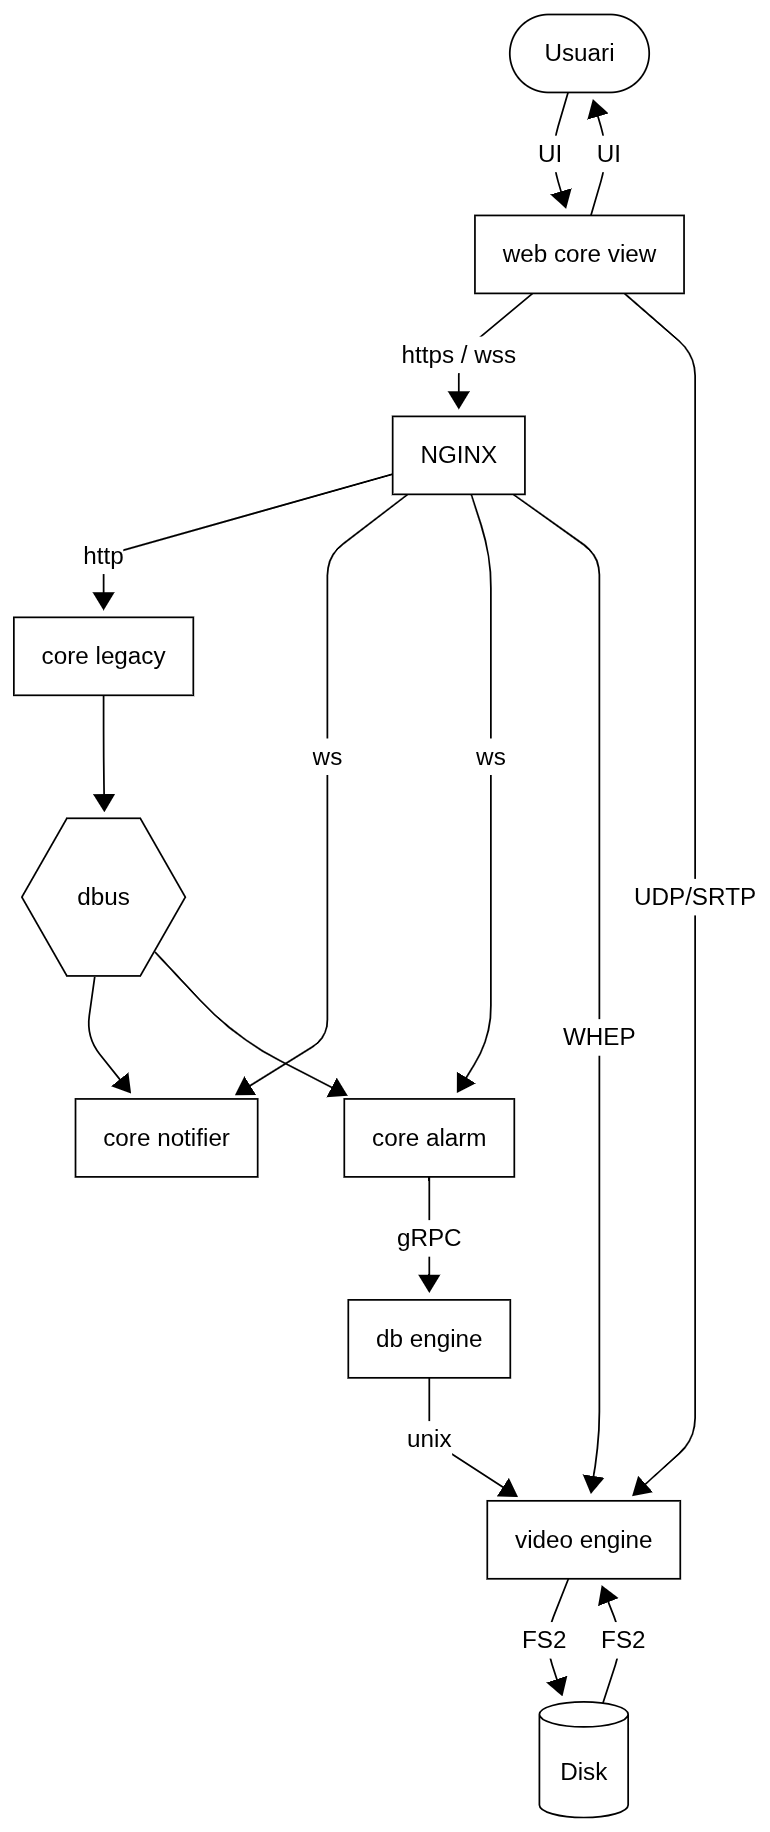
\includegraphics[width=0.9\textwidth, height=0.85\textheight, keepaspectratio]{figures/diagrames/arquitectura_serveis.png}
  \caption{Relació i comunicació entre els serveis de l'NVR.}
  \label{fig:arquitectura_serveis}
  \small Font: Elaboració pròpia.
\end{figure}

\clearpage
\subsection{Capa de comunicació i Proxy}

Per comunicar la web amb els serveis de manera segura, s'interposa \textbf{NGINX} com a \textit{proxy} invers i porta d'entrada única (\textit{gateway}) al sistema. NGINX escolta als ports \texttt{60080} (HTTP) i \texttt{60443} (HTTPS/SSL), i assumeix quatre responsabilitats principals: gestiona el xifratge TLS (protocols TLSv1.2 i TLSv1.3, xifrat \texttt{EECDH+AESGCM}), aplica capçaleres de seguretat HTTP (\texttt{Strict-Transport-Security}, \texttt{X-Frame-Options: SAMEORIGIN}, \texttt{X-Content-Type-Options: nosniff}), controla l'autenticació de les rutes protegides mitjançant el mecanisme intern \texttt{auth\_request}, i enruta cada petició cap al microservei intern corresponent en funció de la ruta URL. Des del punt de vista del navegador, tots els serveis queden amagats darrere una única adreça.

La configuració NGINX agrupa les rutes en quatre blocs funcionals:

\begin{itemize}
    \item \textbf{Configuració i control (HTTPS):} La gran majoria de les rutes —\texttt{/api.rest/}, \texttt{/webprotocol/}, \texttt{/onvif/}, \texttt{/device-service/} i els nombrosos \textit{endpoints} \texttt{.cgi}— es deriven cap a \textbf{la-core-legacy} (port intern \texttt{60088}). Aquest servei centralitza la gestió de la configuració, l'autenticació i el control del sistema.

    \item \textbf{Canals de temps real (WSS):} Les connexions WebSocket persistents segueixen dues rutes diferenciades: \texttt{/ws/la-core-notifier/} es deriven cap al port \texttt{60070} (\textbf{la-core-notifier}), i \texttt{/ws/la-core-alarm/} cap al port \texttt{60071} (\textbf{la-core-alarm}). Ambdós serveis envien esdeveniments en temps real al \textit{frontend} —pèrdues de vídeo, activació de relés, alarmes de sensor— sense que el client hagi de fer \textit{polling}.

    \item \textbf{Vídeo en temps real:} S'ofereixen dos mecanismes de \textit{streaming} gestionats per \textbf{MediaMTX}: el camí \texttt{/stream/} (port \texttt{60889}) serveix vídeo via WebRTC, amb senyalització sobre WebSocket i transport de mitjana SRTP/UDP negociat per ICE; el camí \texttt{/hls/} (port \texttt{60888}) serveix el mateix vídeo en format HLS per a clients que no suporten o tenen dificultats amb WebRTC. 

    \item \textbf{Serveis auxiliars:} El camí \texttt{/video-engine/} enruta directament cap a \textbf{la-video-engine} (port \texttt{60890}) per a operacions de control i consulta del motor de vídeo. El camí \texttt{/db-engine/} connecta amb \textbf{la-db-engine} (port \texttt{60891}) per a consultes de dades històriques. El camí \texttt{/terminal/} connecta amb el servei \textbf{ttyd} (port \texttt{7681}), que ofereix una terminal interactiva accessible directament des del navegador.
\end{itemize}

Per tal de sintetitzar la interacció entre els components, a la Taula \ref{tab:matriu_comunicacio} es detallen els protocols i la naturalesa del trànsit entre el navegador i el gravador:

\begin{table}[htbp]
  \centering
  \caption{Matriu de comunicació de la plataforma.}
  \label{tab:matriu_comunicacio}
  \resizebox{\textwidth}{!}{
  \begin{tabular}{@{}lllll@{}}
    \toprule
    \textbf{Origen} & \textbf{Destinació (Servei)} & \textbf{Ruta NGINX} & \textbf{Protocol} & \textbf{Finalitat} \\ \midrule
    Navegador & NGINX $\rightarrow$ \textbf{la-core-legacy} & \texttt{/login/}, \texttt{/(en|es|fr)/} & HTTPS & Descàrrega de l'aplicació Angular (SPA) \\
    Navegador & NGINX $\rightarrow$ \textbf{la-core-legacy} & \texttt{/api.rest/}, \texttt{/webprotocol/}, \texttt{*.cgi} & HTTPS & Configuració, autenticació i control del sistema \\
    Navegador & NGINX $\rightarrow$ \textbf{la-core-notifier} & \texttt{/ws/la-core-notifier/} & WSS & Notificacions de sistema en temps real \\
    Navegador & NGINX $\rightarrow$ \textbf{la-core-alarm} & \texttt{/ws/la-core-alarm/} & WSS & Notificacions d'alarmes en temps real \\
    Navegador & NGINX $\rightarrow$ \textbf{MediaMTX} & \texttt{/stream/} & WSS + SRTP/UDP & Vídeo en directe via WebRTC \\
    Navegador & NGINX $\rightarrow$ \textbf{MediaMTX} & \texttt{/hls/} & HTTPS & Vídeo en directe via HLS \\
    Navegador & NGINX $\rightarrow$ \textbf{la-video-engine} & \texttt{/video-engine/} & HTTPS & Control i consulta del motor de vídeo \\
    Navegador & NGINX $\rightarrow$ \textbf{la-db-engine} & \texttt{/db-engine/} & HTTPS & Consultes de dades històriques \\
    Navegador & NGINX $\rightarrow$ \textbf{ttyd} & \texttt{/terminal/} & WSS & Terminal interactiva via navegador \\
    % \textbf{la-core-notifier} / \textbf{la-core-alarm} & \textbf{la-db-engine} & — & gRPC / D-Bus & Comunicació interna del backend \\
    % \textbf{la-video-engine} & \textbf{la-db-engine} & — & Unix Sockets & Persistència al disc (VFS SQLite) \\ \bottomrule
  \end{tabular}
  }
\end{table}

\clearpage
El Llistat \ref{lst:nginx_routing} mostra els blocs de configuració NGINX que implementen les rutes principals de la plataforma, extrets directament del fitxer \texttt{la-core.conf} del repositori de build \textbf{mantos-rec} (\texttt{sources/meta-mantos/recipes-httpd/nginx/nginx/la-core.conf}):

\begin{lstlisting}[language=bash, label={lst:nginx_routing}, caption={Fragment de la configuració NGINX (la-core.conf, repositori mantos-rec): rutes principals de la plataforma.}]
# Aplicacio Angular (SPA) - requereix autenticacio
location ~ ^/(en|es|fr)/ {
    auth_request /auth.cgi;
    error_page 401 = @error401;
    alias /data/web-core-view/var/www/browser/;
    try_files $uri $uri/ /login/index.html;
}

# WebSocket - Notificacions generals del sistema
location /ws/la-core-notifier/ {
    proxy_pass http://localhost:60070/;
    proxy_http_version 1.1;
    proxy_set_header Upgrade $http_upgrade;
    proxy_set_header Connection "upgrade";
    proxy_send_timeout 600s;
    proxy_read_timeout 600s;
}

# WebSocket - Canal d'alarmes
location /ws/la-core-alarm/ {
    proxy_pass http://localhost:60071/;
    proxy_http_version 1.1;
    proxy_set_header Upgrade $http_upgrade;
    proxy_set_header Connection "upgrade";
    proxy_send_timeout 600s;
    proxy_read_timeout 600s;
}

# Motor de video - control i consulta (protegit per auth)
location /video-engine/ {
    auth_request /auth.cgi;
    error_page 401 = @error401;
    proxy_http_version 1.1;
    proxy_pass http://localhost:60890/;
}

# Base de dades - dades historiques (protegit per auth)
location /db-engine/ {
    auth_request /auth.cgi;
    error_page 401 = @error401;
    proxy_http_version 1.1;
    proxy_pass http://localhost:60891/;
}

# Streaming WebRTC via MediaMTX (protegit per auth)
location /stream/ {
    auth_request /auth.cgi;
    error_page 401 = @error401;
    proxy_pass http://localhost:60889/stream/;
    proxy_http_version 1.1;
    proxy_set_header Upgrade $http_upgrade;
    proxy_set_header Connection "upgrade";
}
\end{lstlisting}

% Per resoldre aquest desacoblament a l'hora d'enviar esdeveniments, s'ha dissenyat un mecanisme de \textbf{bridging de protocols (Protocol Bridging)} centralitzat en el servei de notificacions (\textit{Core Notifier}) del gravador. Aquest servei actua com a intermediari actiu (\textit{gateway}): es subscriu als esdeveniments de sistema (com pèrdues de vídeo o activació de relés) mitjançant el bus D-Bus i canals gRPC, tradueix aquestes estructures de baix nivell en missatges JSON lleugers i, finalment, els transmet en temps real pel canal de \textbf{WebSockets} (WSS) \cite{rfc6455} fins al client Angular. Aquest disseny garanteix que el frontend pugui respondre immediatament a qualsevol esdeveniment de seguretat, sense connexions binàries natives costoses ni sobrecàrrega de la CPU del client.

\clearpage
\subsection{Seguretat Defensiva contra vectors d'atac OWASP}
Com a requisit no funcional de seguretat crítica, el frontend s'ha dissenyat per mitigar de forma activa les principals vulnerabilitats del catàleg OWASP Top 10. La gestió de la sessió s'ha dissenyat per eliminar tots els vectors de robatori de credencials: les \textit{cookies} de sessió es gestionen amb els atributs \texttt{HttpOnly} i \texttt{Secure} configurats exclusivament a la capa de NGINX, de manera que resten completament inaccessibles des de qualsevol codi JavaScript del client i, per tant, immunitzades contra atacs de tipus \textit{Cross-Site Scripting} (XSS). La prevenció de \textit{Cross-Site Request Forgery} (CSRF) s'aconsegueix gràcies a la política \textit{Same-Origin} imposada per NGINX i a la naturalesa \textit{zero-persistence} del Signal privat d'estat en memòria del \textit{frontend}: un recarregament de pàgina invalida la sessió al costat del client sense necessitat de cap \textit{token} CSRF addicional.

Addicionalment, a la capa de NGINX, s'ha unificat l'origen de l'aplicació i l'API REST sota un mateix servidor de recursos, cosa que permet aplicar polítiques de \textit{Same-Origin} estrictes que limiten els vectors d'injeccions \textit{Cross-Site Scripting} (XSS) i els intents de \textit{Clickjacking}.

L'ús de NGINX com a \textit{entry point} és indispensable per a la seguretat del sistema. En centralitzar les peticions, NGINX actua de tallafoc per als serveis \textbf{la-video-engine} i \textbf{la-core-legacy}, impedint l'accés directe als ports interns. A més, permet que el token JWT generat per l'autenticació sigui vàlid per a tots els microserveis sota un mateix domini de seguretat, simplificant la gestió de capçaleres \textit{Authorization} i evitant problemes de CORS (Cross-Origin Resource Sharing) que podrien bloquejar l'streaming de vídeo.

\begin{lstlisting}[language=bash, label={lst:nginx_security}, caption={Fragment de la configuració NGINX (la-core.conf): TLS i capçaleres de seguretat HTTP.}]
server {
    listen 60080;
    listen 60443 ssl;

    # Certificats TLS del dispositiu
    ssl_certificate     /etc/ssl/certs/la-certificate.crt;
    ssl_certificate_key /etc/ssl/private/la-certificate.key;

    # Protocols i xifrats forts (OWASP TLS Cheat Sheet)
    ssl_protocols             TLSv1.2 TLSv1.3;
    ssl_prefer_server_ciphers on;
    ssl_dhparam               /etc/nginx/la-dhparam.pem;
    ssl_ciphers               EECDH+AESGCM:EDH+AESGCM;
    ssl_ecdh_curve            secp384r1;
    ssl_session_timeout       10m;
    ssl_session_cache         shared:SSL:10m;
    ssl_session_tickets       off;
    ssl_stapling              on;
    ssl_stapling_verify       on;

    # Capçaleres de seguretat HTTP
    add_header Strict-Transport-Security
               "max-age=31536000; includeSubDomains" always;
    add_header X-Frame-Options        "SAMEORIGIN" always;
    add_header X-Content-Type-Options "nosniff"    always;
    add_header Referrer-Policy
               "strict-origin-when-cross-origin"   always;
}
\end{lstlisting}

\section{Disseny del Frontend (Angular 19)}
L'elecció d'Angular 19 no és casual; el \textit{framework} proporciona una estructura que facilita el manteniment a llarg termini de l'aplicació.

\begin{figure}[htbp]
  \centering
  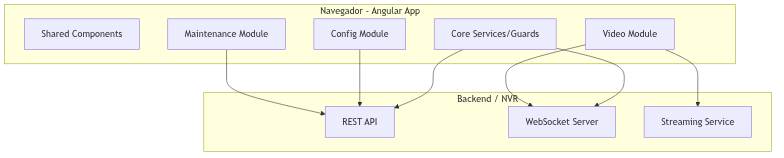
\includegraphics[width=0.85\textwidth]{figures/angular_components.png}
  \caption{Diagrama de components de l'arquitectura de l'aplicació Angular i la seva integració amb el backend.}
  \label{fig:angular_components}
  \small Font: Elaboració pròpia.
\end{figure}

\subsection{Arquitectura Modular i Standalone Components}
S'ha eliminat l'ús de mòduls clàssics d'Angular en favor dels \textit{Standalone Components}. Això redueix el \textit{boilerplate} del codi i millora el temps de càrrega de l'aplicació (\textit{lazy loading}), ja que només es descarreguen al navegador els components necessaris per a la vista actual (per exemple, el mòdul de configuració avançada no es carrega si l'usuari només vol veure vídeo).

L'organització d'aquests elements quant a dependències i estructura de mòduls es presenta gràficament a la Figura \ref{fig:angular_modules}.

\begin{figure}[!htbp]
  \centering
  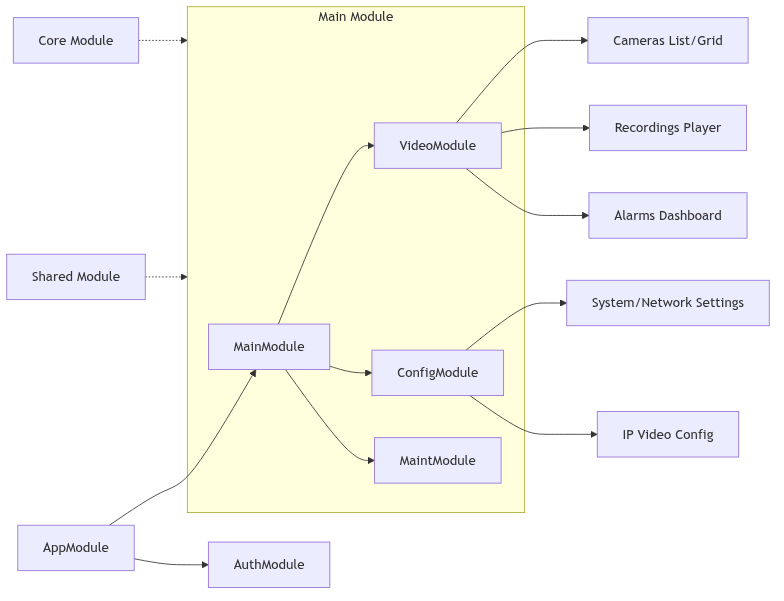
\includegraphics[width=0.75\textwidth, height=0.45\textheight, keepaspectratio]{figures/angular_modules.png}
  \caption{Diagrama de mòduls de l'aplicació Angular i relació amb els components compartits i serveis de la capa Core.}
  \label{fig:angular_modules}
  \small Font: Elaboració pròpia.
\end{figure}

\subsection{Gestió de l'Estat amb Angular Signals}
Aquest és un punt d'inflexió respecte a les versions anteriors del programari. Mentre que RxJS és excel·lent per a fluxos de dades complexos, \textbf{Angular Signals} permet una reactivitat granular \cite{learning_angular}.
\begin{itemize}
    \item \textbf{Eficiència:} En un sistema de vigilància on els estats de les càmeres canvien constantment, els \textit{Signals} asseguren que només es torni a renderitzar la part mínima de l'arbre del DOM afectada, reduint dràsticament l'ús de CPU al terminal del client.
    \item \textbf{Sincronització:} Els valors calculats (\textit{computed signals}) faciliten que la interfície s'adapti automàticament a canvis en el \textit{lock} de configuració o en l'estat de connectivitat informat pel \textit{Keep-alive}.
\end{itemize}

Dins d'aquest disseny de gestió d'estat reactiu, un dels reptes tècnics ha estat la modificació d'estructures de dades altament anidades zone-free sense trencar la detecció de canvis nativa. Angular Signals es basa en la comparació de valors per referència; per tant, mutar directament una propietat interna d'un objecte complex no dispararia la reactivitat del component. Per resoldre-ho, s'ha implementat un algorisme de manipulació profunda (\textit{deep copy} i \textit{deep access}) que clona l'objecte d'estat local completament, hi aplica la modificació en el camp editat dinàmicament (identificat pel camí de la propietat JSON de l'esquema), i finalment actualitza el Signal amb la nova referència (\texttt{configSignal.set(newConfig)}). Aquest disseny garanteix la immutabilitat de l'estat i evita defectes de renderitzat col·laterals.

A diferència de les arquitectures anteriors basades en \texttt{Zone.js}, que havien de revisar tot l'arbre de components davant qualsevol esdeveniment, l'ús de \textbf{Signals} permet que l'aplicació s'apropi a un model \textit{Zone-less} (amb l'ús puntual de \texttt{NgZone} per a operacions concretes que ho requereixen, com ara els temporitzadors del servei de \textit{keep-alive}). Això és especialment crític en la visualització de vídeo: el fet que arribin metadades cada 100ms sobre el bitrate no provoca que es torni a avaluar tota la interfície, sinó només l'etiqueta de text específica, alliberant cicles de CPU del terminal per dedicar-los exclusivament a la descodificació de vídeo H.265.

\section{El Motor Schema-Driven}
El component més innovador del sistema és el motor de configuració dinàmic. Aquest motor permet desacoblar totalment el desenvolupament del \textit{frontend} de l'evolució del \textit{firmware}.

\subsection{Lògica de funcionament}
En lloc de programar pantalles de configuració estàtiques, s'ha creat un intèrpret que segueix aquest flux:
\begin{enumerate}
    \item \textbf{Recepció del Schema:} El gravador envia un fitxer JSON que descriu les propietats (tipus de dades, límits, valors per defecte i dependències).
    \item \textbf{Parseig:} El servei \texttt{ConfigInputComponent} processa la metadada i mapeja cada propietat a un component visual (un \textit{toggle} per a booleans, un \textit{slider} per a sensibilitat, etc.).
    \item \textbf{Manipulació de camins:} S'utilitzen utilitats de \textit{Deep Access} per llegir i escriure en estructures d'objectes anidats (ex: \texttt{config.io.outputs[0].task}), garantint que l'enviament de tornada al servidor sigui un node vàlid.
\end{enumerate}

Aquest enfocament és especialment valuós quan s'introdueixen noves funcionalitats a \textbf{la-video-engine} o \textbf{la-core-alarm}. En lloc de programar una nova vista a Angular, el servei de backend simplement actualitza el seu esquema de dades i el \textit{frontend} el renderitza automàticament, reduint el temps de \textit{time-to-market} de noves versions del firmware.

És important destacar que el servei \textbf{la-core-legacy} és el responsable de generar aquest esquema dinàmic. El servei inspecciona les capacitats del maquinari (nombre de canals de vídeo, tipus de ports instal·lats) i construeix el diccionari de metadades JSON en temps real. Això permet que una mateixa versió de la interfície web sigui capaç de gestionar tant un gravador compacte de 4 càmeres com una unitat de rack de 64 càmeres, ja que el \textit{frontend} no té el nombre d'interfícies codificat de manera estàtica, sinó que es limita a renderitzar allò que \textbf{la-core-legacy} li indica.

Un dels reptes d'aquest disseny és la \textbf{tolerància a errors en l'esquema}. S'ha implementat una lògica de \textit{fail-safe} al frontend: si \textbf{la-core-legacy} envia un node de configuració amb un tipus no reconegut o amb paràmetres fora de rang, el motor no bloqueja el renderitzat de la resta de la pàgina. En lloc d'això, substitueix el component defectuós per un avís visual de 'Paràmetre no compatible', permetent que l'operador continuï treballant amb la resta del sistema sense patir un tancament inesperat de l'aplicació.

\section{Disseny de la Persistència i dades}
Tot i que el sistema és principalment una interfície de gestió, l'arquitectura preveu la persistència en dos nivells:
\begin{itemize}
    \item \textbf{SQLite3:} Utilitzada en el costat del servidor (\textit{backend embedded}) per a la gestió ràpida de l'historial d'alarmes i la configuració persistent dels usuaris.
    \item \textbf{Estratègia de Buffering:} El \textit{frontend} gestiona un estat local temporal per permetre a l'usuari realitzar múltiples canvis i validar-los abans d'adquirir el \textit{lock} i enviar la configuració final al maquinari.
\end{itemize}

\subsection{Model de dades de l'aplicació}
Per tal de representar la correspondència i relació entre les diferents estructures de dades que es reben de l'API (com ara Càmeres, Codecs, Presets o Alarmes), s'ha elaborat un model d'entitats representat en el diagrama de classes de la Figura \ref{fig:class_diagram}. Cal destacar que el model de la classe \texttt{Camera} està dissenyat per reflectir exactament l'estructura tipada del \textit{frontend} en TypeScript, incloent l'objecte imbricat \texttt{ipConfig}, el qual conté camps clau com \texttt{manufacturer} i \texttt{model}. Aquests camps són essencials per a la renderització correcta de les taules de manteniment i la generació d'informes tècnics d'estat de l'equip.

\begin{figure}[!htbp]
  \centering
  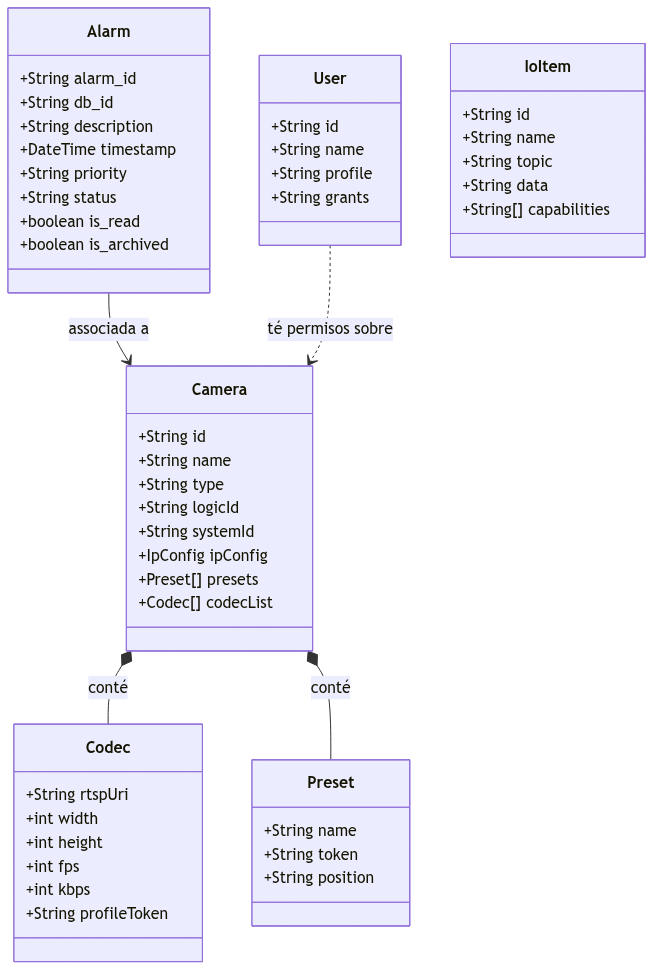
\includegraphics[width=0.75\textwidth, height=0.45\textheight, keepaspectratio]{figures/class_diagram.png}
  \caption{Diagrama de classes de les entitats principals del sistema WebCoreView.}
  \label{fig:class_diagram}
  \small Font: Elaboració pròpia.
\end{figure}
\chapter{Implementació}
\label{ch:implementacio}

En aquest capítol es detalla el procés de construcció del sistema \textit{Web Core View}. Es descriu l'entorn de treball i s'explora el funcionament tècnic de cada mòdul al mateix temps que s'analitza la seva interfície gràfica d'usuari (UI). Aquest recorregut pràctic permet entendre com els requisits funcionals i l'arquitectura de \textit{software} s'han traduït en una experiència d'usuari intuïtiva.

\section{Entorn de desenvolupament i tecnologies}
Per a la implementació del \textit{frontend}, s'ha configurat un entorn basat en \textbf{Node.js} i l'ecosistema \textbf{Angular CLI 19}. L'estructura del projecte s'ha dissenyat basant-se en components completament independents, una decisió que permet simplificar notablement el codi i assegurar que l'aplicació web carregui d'una manera molt més ràpida al navegador.

Pel que fa als estils, s'ha utilitzat \textbf{SCSS modular}. S'han definit variables globals per mantenir la consistència visual i s'ha aplicat l'estratègia de detecció de canvis \texttt{OnPush} per garantir que la interfície només es refresqui quan realment hi hagi canvis d'estat significatius.

\section{Autenticació, Gestió de Permisos i Cicle de Vida del Core}
El primer punt de contacte de l'usuari amb el sistema és la pantalla d'inici de sessió (Figura \ref{fig:ui_login}). A diferència d'altres plataformes de gestió web, en tractar-se d'un sistema \textit{embedded} de seguretat crítica, el flux de treball s'ha dissenyat per minimitzar el consum de recursos al microcontrolador local sense comprometre el control d'accessos ni la robustesa de la sessió.

\begin{figure}[htbp]
  \centering
  
\includegraphics[width=0.85\textwidth]{figures/ui_login.png}
  \caption{Pantalla d'inici de sessió (Login).}
  \label{fig:ui_login}
\end{figure}

L'API d'autenticació del sistema s'executa com un procés en dues fases coordinat a través del punt d'accés unificat \texttt{/WebLogin}, gestionat pel microservei \textbf{la-core-legacy} i exposat a l'exterior de forma segura mitjançant el proxy invers d'NGINX sota el protocol de transport xifrat HTTPS.

\subsection{Fase 1: Verificació de credencials (PlainLogin)}
El client envia les credencials introduïdes per l'operador. Tot i que viatgen en text pla dins del JSON, la confidencialitat està garantida pel xifrat de la capa de transport (HTTPS/TLS). S'efectua una petició HTTP POST a \texttt{/WebLogin} enviant el següent payload:

\begin{lstlisting}[language=json, caption={Petició d'enviament de credencials al servidor (PlainLogin).}]
{
  "call": "PlainLogin",
  "User": "admin",
  "Password": "LaTevaContrasenya"
}
\end{lstlisting}

Depenent de la validesa de les credencials o de l'estat de seguretat del compte, el servidor pot retornar tres escenaris diferents:

\begin{itemize}
  \item \textbf{Autenticació reeixida (Success):} El servidor valida les credencials, estableix un \textit{cookie} de sessió segur gestionat nativament pel navegador (mitjançant polítiques \textit{Same-Origin} i atributs \textit{HttpOnly} configurats a NGINX) i retorna una resposta d'èxit.
  \item \textbf{Credencials incorrectes (Unauthorized):} Es denega l'accés i es retorna el nombre d'intents restants abans del bloqueig del compte.
  \item \textbf{Compte bloquejat (Locked):} Si s'ha superat el límit de 5 intents fallits, el servei bloqueja les peticions d'aquest usuari de forma temporal durant 15 minuts.
\end{itemize}

\begin{lstlisting}[language=json, caption={Exemples de resposta segons l'escenari d'autenticació.}]
// Cas A: Success
{ "LoginResponse": "success", "RetryCount": null }

// Cas B: Unauthorized
{ "LoginResponse": "unauthorized", "RetryCount": "3" }

// Cas C: Locked
{ "LoginResponse": "locked", "RetryCount": "0" }
\end{lstlisting}

\subsection{Fase 2: Obtenció del context i resolució de permisos (GetWhoamI)}
Un cop es rep la confirmació d'èxit de la Fase 1, l'aplicació s'ha d'inicialitzar. Com que les dades de sessió no s'emmagatzemen al magatzem local (\textit{LocalStorage}) per tal d'evitar atacs de tipus \textit{Cross-Site Scripting} (XSS) i robatoris de credencials, el frontend utilitza l'estat asíncron establert pel navegador mitjançant la gestió nativa de \textit{cookies}.

El component de \textit{login} invoca el mètode \texttt{onInitPage()} de l'injector \texttt{UserService}, el qual realitza una nova petició POST cap a \texttt{/WebLogin} sota el mètode de control de context \texttt{GetWhoamI}:

\begin{lstlisting}[language=json, caption={Petició d'obtenció de perfil i permisos del context d'usuari.}]
// Petició
{
  "call": "GetWhoamI"
}

// Resposta
{
  "user": "admin",
  "profile": "administrator",
  "grants": "configuration+live+record+managment+users"
}
\end{lstlisting}

Aquesta resposta conté els permisos explícits (\textit{grants}) de l'usuari. Aquests es divideixen en un diccionari del costat de client que s'utilitza per mapar les funcionalitats i ocultar o mostrar elements del DOM en temps real:

\begin{itemize}
  \item \textbf{configuration:} Permet accedir als menús de configuració de xarxa, rellotge, entrades/sortides físiques i virtuals, i alarmes.
  \item \textbf{users:} Habilita l'edició de comptes de tercers usuaris, actualització de contrasenyes i definició de permisos de perfil.
  \item \textbf{live:} Autoritza la visualització de vídeo en temps real de les càmeres IP connectades. Si s'utilitza en combinació amb el grant \textit{live-limited}, l'accés es restringeix exclusivament als canals indicats al camp \texttt{visual-cams} de la seva fitxa d'usuari.
  \item \textbf{record / download:} Habilita la consulta, reproducció històrica (\textit{playback}) i descàrrega de fragments d'enregistrament de vídeo emmagatzemats als discs durs del gravador.
  \item \textbf{managment:} Permet accedir a la descàrrega del fitxer de registre d'auditories (\textit{logs}), a la documentació interna i a les còpies de seguretat de la configuració.
  \item \textbf{firmware:} Permet realitzar l'actualització del microprogramari del dispositiu des del panell de manteniment.
\end{itemize}

El token i les credencials de sessió es mantenen exclusivament en l'estat en memòria d'un \textbf{Signal privat} dins de la capa del servei d'Angular 19, seguint un model estricte de \textit{zero-persistence}. El cost d'aquest disseny és que un refresc manual de la pàgina (\texttt{F5}) tanca la sessió, una penalització menor d'experiència d'usuari (UX) que es considera un requisit de seguretat desitjable i necessari en entorns industrials crítics.

\begin{figure}[htbp]
  \centering
  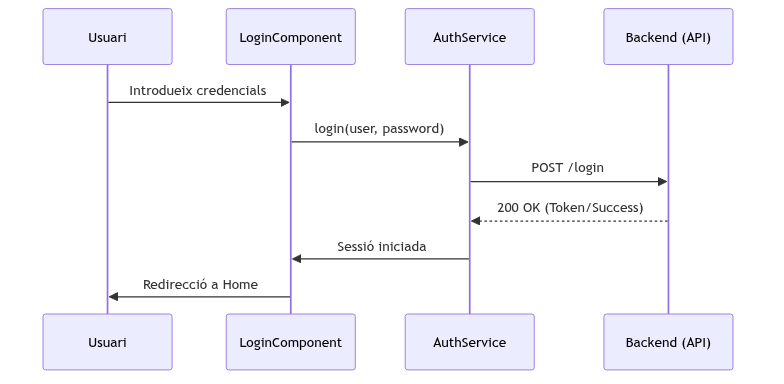
\includegraphics[width=0.85\textwidth]{figures/seq_login.png}
  \caption{Diagrama de seqüència del flux de control d'inici de sessió.}
  \label{fig:seq_login}
  \small Font: Elaboració pròpia.
\end{figure}

\subsection{L'Interceptor de Bloqueig i el Control de Concurrència}
Cal destacar que l'aplicació Angular implementa l'interceptor funcional d'Angular 19 \texttt{authInterceptor} (vegeu el llistat \ref{lst:auth_interceptor_code}). Tanmateix, a diferència de les aplicacions web convencionals on l'interceptor afegeix un token d'usuari, a \textit{Web Core View} aquest s'encarrega d'injectar de forma dinàmica el token de bloqueig d'escriptura (\textbf{Config Lock Token}) adquirit des del servei \texttt{ConfigLockService}. Això assegura que les peticions modificatives cap a les APIs de configuració (\texttt{config.video.*}, \texttt{config.io.*}) estiguin autoritzades per l'exclusivitat del cadenat.

\begin{lstlisting}[language=JavaScript, label={lst:auth_interceptor_code}, caption={Implementació del HttpInterceptorFn per al control del Config Lock en Angular 19.}]
export const authInterceptor: HttpInterceptorFn = (req, next) => {
  const lockService = inject(ConfigLockService);
  const token = lockService.lockToken();
  const isConfigApi = req.url.includes('/config.') || req.url.includes('/resources');
  const isLockOrUnlock = req.url.includes('/properties/lock') || req.url.includes('/properties/unlock');

  if (token && isConfigApi && !isLockOrUnlock) {
    const modifiedReq = req.clone({
      setParams: { token: token }
    });
    return next(modifiedReq);
  }
  return next(req);
};
\end{lstlisting}

\subsection{Subscripció Asíncrona de Temps Real i Notificacions}
Immediatament després d'un inici de sessió reeixit i la redirecció de l'operador cap a la pàgina d'inici de l'aplicació (\texttt{/home}), s'inicialitza la comunicació bidireccional amb el microservei unificat de notificacions. L'aplicació obre un únic canal persistent via WebSocket Segur (\textbf{WSS}) cap al camí \texttt{/ws/la-core-notifier/}.

Aquesta connexió asíncrona unificada és fonamental per rebre d'una sola vegada totes les notificacions de canvis d'estats dels sensors digitals d'E/S, errors globals del maquinari i alertes de pèrdues de senyal de vídeo, evitant que diferents components de la interfície facin peticions redundants o mantinguin múltiples túnels oberts (la qual cosa saturaria la capacitat del gravador).

\subsection{Mecanisme de Keep-Alive i Heartbeat de Sessió}
El manteniment de la sessió es coordina entre el client i el microservei \textbf{la-core-legacy} a través de la persistència del \textit{Heartbeat} emès pel servei \texttt{KeepAliveService}. Aquest mètode executa una crida POST cap al mètode \texttt{KeepAliveSession} de forma periòdica cada 60 segons:

\begin{lstlisting}[language=json, caption={Trama de Keep-Alive enviada periòdicament al servidor.}]
{
  "call": "KeepAliveSession"
}
\end{lstlisting}

\section{Tauler Principal i Panells d'Informació}
La pàgina d'inici (\textit{Home page}) actua com el nucli d'operacions i el despatxador logístic de la plataforma. És la primera interfície que l'operador visualitza un cop el sistema valida correctament les seves credencials en el flux d'autenticació (Figura \ref{fig:ui_home}).

\begin{figure}[htbp]
  \centering
  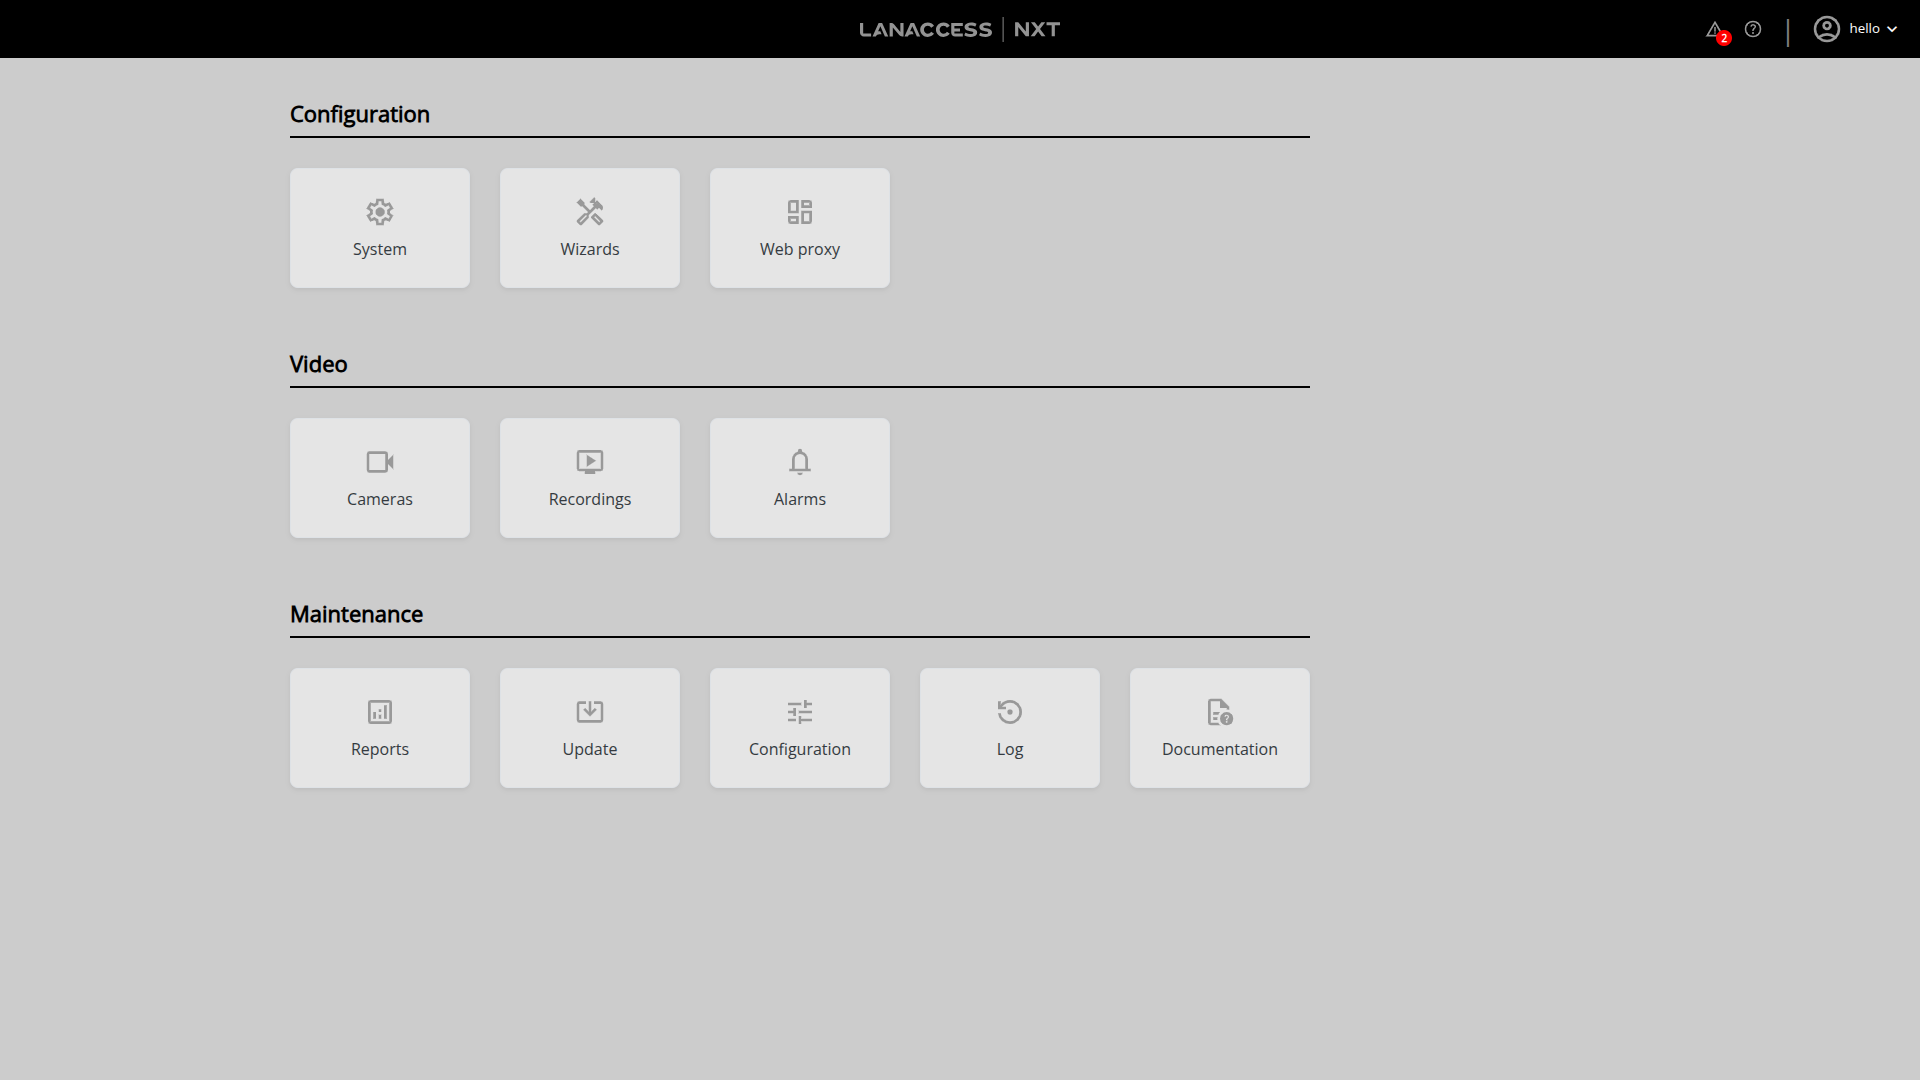
\includegraphics[width=0.95\textwidth]{figures/ui_home.png}
  \caption{Pàgina d'inici principal de Web Core View.}
  \label{fig:ui_home}
\end{figure}

Des d'aquesta pantalla centralitzada, l'usuari pot navegar de manera asíncrona mitjançant el menú de mosaic o utilitzar els controls globals de la capçalera de l'aplicació per accedir a les diferents eines operatives.

\subsection{Organització de Funcionalitats i Autorització Dinàmica}
Per garantir una experiència d'usuari (UX) neta, adaptada al context de treball i lliure de sobrecàrregues cognitives, les eines del sistema s'organitzen visualment en tres grans seccions funcionals:

\begin{itemize}
  \item \textbf{Configuració:} Reuneix l'accés a la configuració del sistema (\textit{System}), els assistents guiats d'instal·lació (\textit{Wizards}) i l'eina de mapeig de túnels de xarxa per a càmeres aïllades (\textit{Web Proxy}).
  \item \textbf{Vídeo:} Agrupa el visualitzador de càmeres en temps real (\textit{Cameras}), la consulta del reproductor històric de gravacions (\textit{Recordings}) i la consola de supervisió d'incidents actius (\textit{Alarms}).
  \item \textbf{Manteniment:} Conté els mòduls de diagnòstic avançat (\textit{Reports}), actualització del microprogramari (\textit{Update}), restauració i còpies de seguretat de fitxers de configuració (\textit{Configuration}), el visor de registres històrics (\textit{Log}) i la descàrrega directa de manuals d'usuari integrats (\textit{Documentation}).
\end{itemize}

L'aspecte més destacable d'aquest disseny és que el motor de renderitzat del *frontend* avalua de forma immediata el mètode reactiu \texttt{functionalities} derivat de la llista de \textit{grants} de l'usuari a través d'Angular Signals. Si l'operador actual manca d'un permís determinat (com ara l'accés a la modificació d'usuaris o a l'actualització de firmware), els botons i rutes d'aquella secció específica s'exclouen directament del cicle de vida del DOM del client. Això no només augmenta la seguretat en l'entorn de treball, sinó que evita la renderització d'elements redundants que l'usuari final no pot utilitzar.

\subsection{Controls Globals i Panells d'Informació de Maquinari i Usuari}
A la part superior dreta de l'aplicació, dins de la barra de capçalera persistent, s'ubiquen els controls d'accés ràpid i els panells flotants en temps real (Figura \ref{fig:ui_home_panels}).

\begin{figure}[htbp]
  \centering
  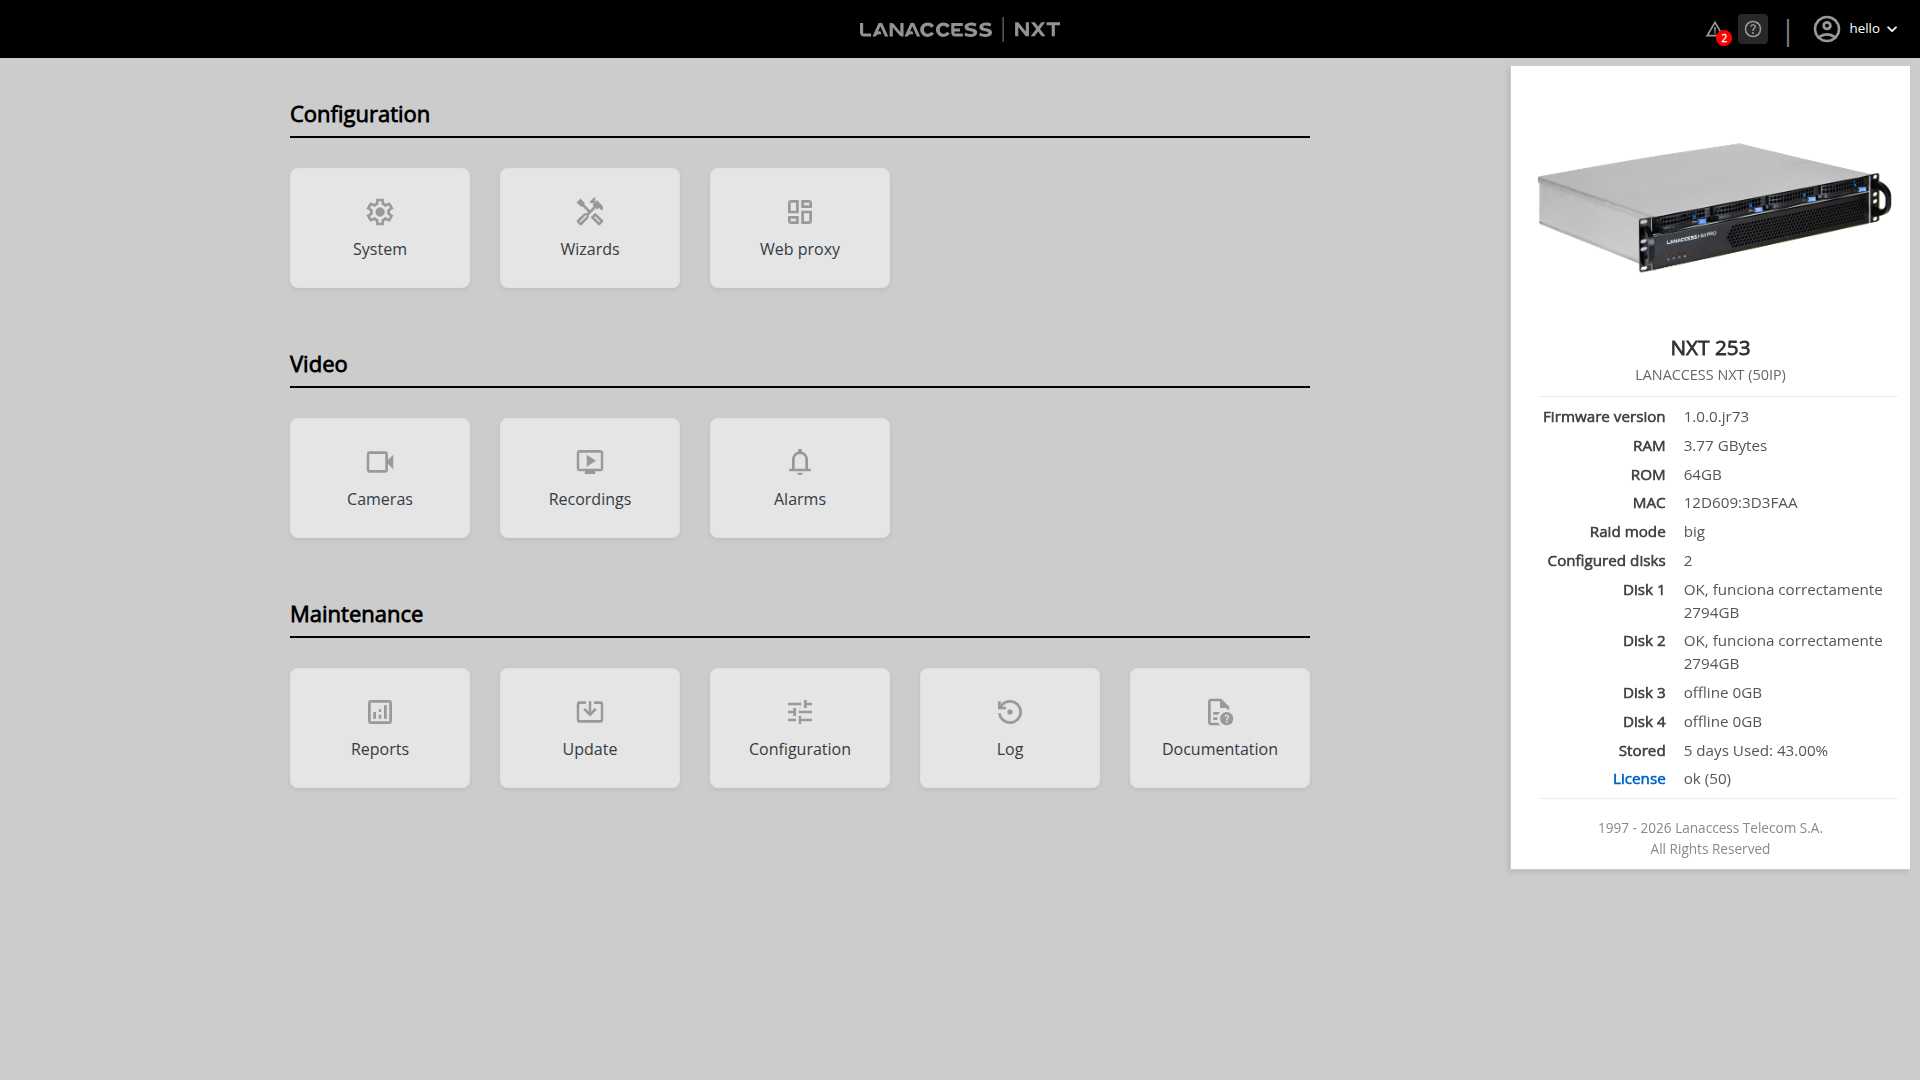
\includegraphics[width=0.45\textwidth]{figures/ui_home_info.png}
  \hfill
  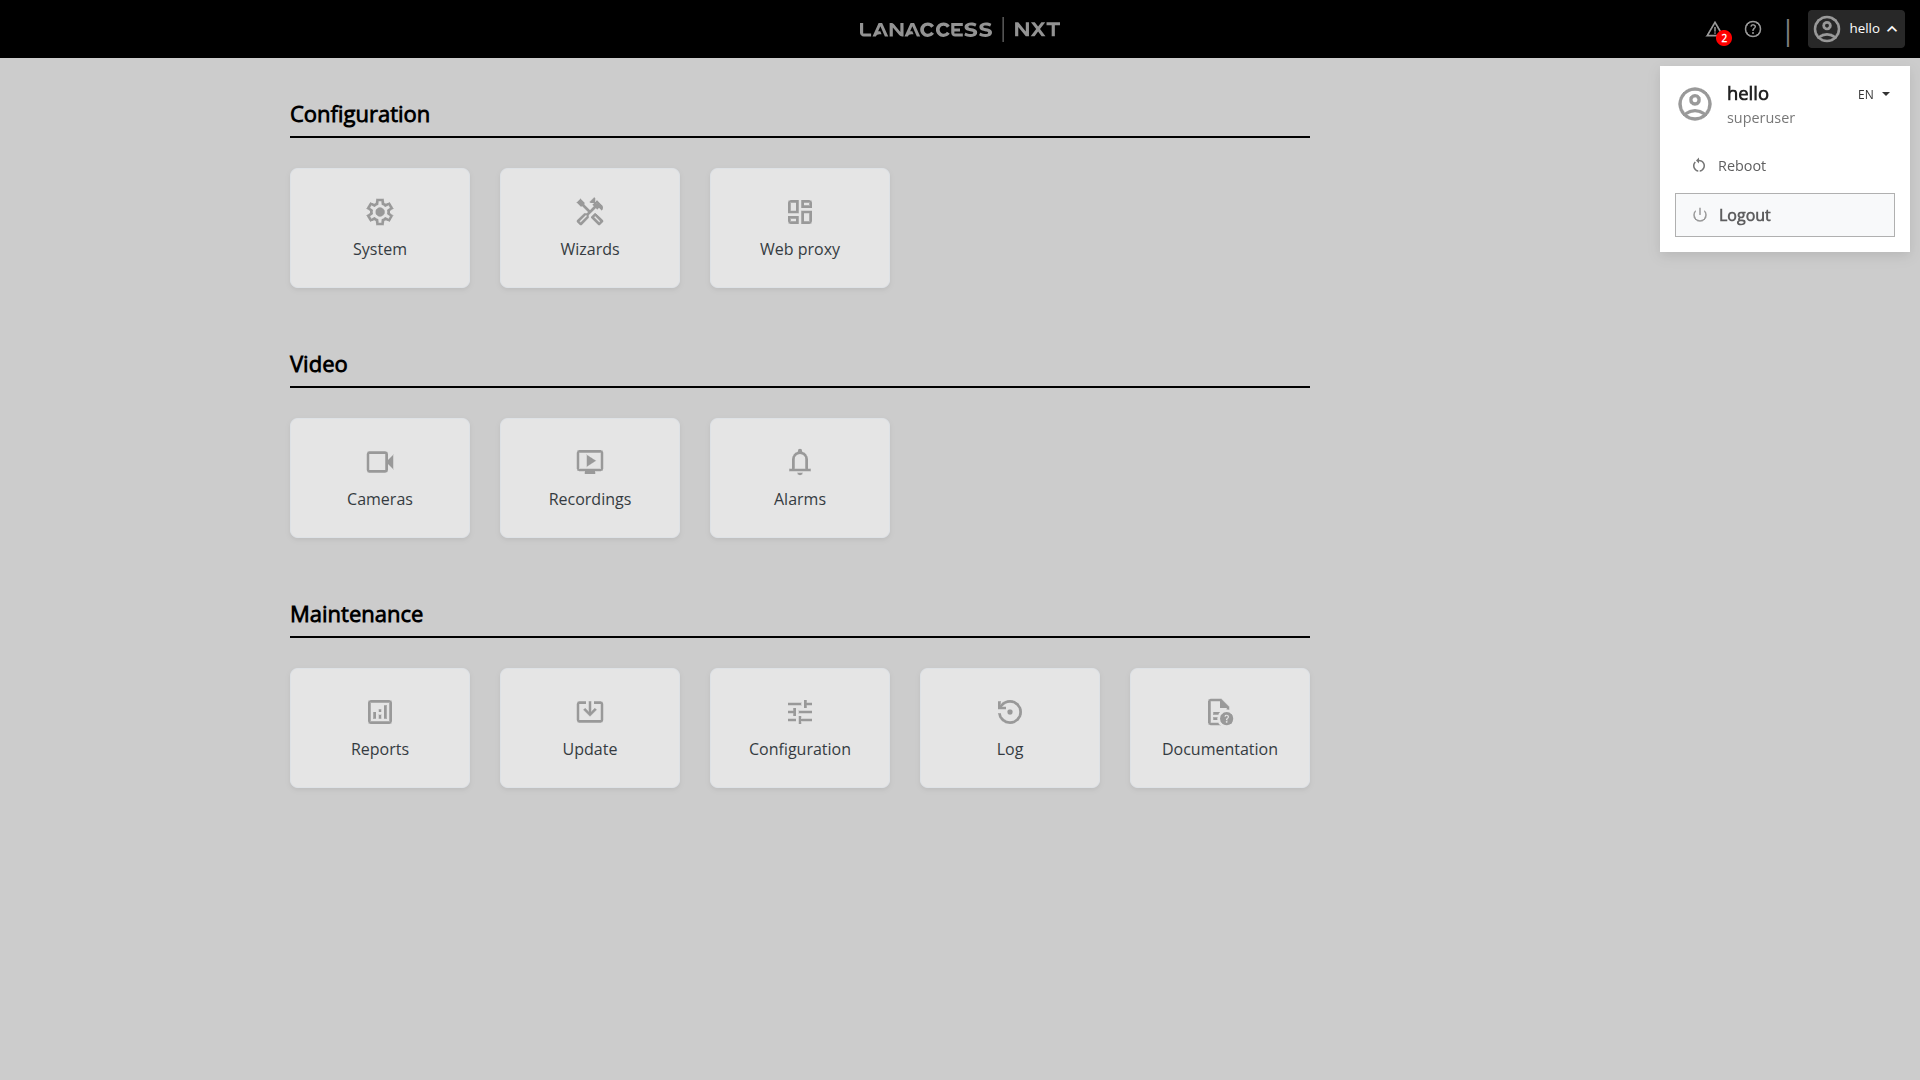
\includegraphics[width=0.45\textwidth]{figures/ui_home_user.png}
  \caption{Panell d'informació de l'estat del videogravador (esquerra) i d'usuari (dreta).}
  \label{fig:ui_home_panels}
\end{figure}

Fent clic a la icona d'informació de maquinari, es desplega un panell lateral que actua com a diagnòstic ràpid de l'estat de salut de l'NVR (Figura \ref{fig:ui_home_panels}, esquerra). Aquest panell mostra paràmetres crítics obtinguts directament del maquinari de forma asíncrona:
\begin{itemize}
  \item Adreça IP local i adreça física MAC de la interfície \texttt{eth0}.
  \item Versió del firmware del sistema operatiu i model del dispositiu de gravació.
  \item \textbf{Estat de l'emmagatzematge físic:} Llista normalitzada dels discos durs muntats al sistema, detallant-ne la capacitat, el model de fabricant, el número de sèrie, el mode de redundància de dades (RAID) actiu i el percentatge d'espai utilitzat.
  \item Temperatura del processador central obtinguda directament dels sensors integrats.
  \item \textbf{Estat de la llicència:} Des d'aquest panell d'informació del videogravador podem veure l'estat actual de la llicència, amb un botó accionable que redirigeix directament a la pàgina de llicència.
\end{itemize}

Per alimentar aquest panell de diagnòstic, el frontend realitza una petició HTTP GET cap a la ruta d'API xifrada \texttt{/webprotocol/config\_data.xml?requests=system+network}. El microservei \textbf{la-core-legacy} s'encarrega d'analitzar les variables del sistema, unificar les metadades en un fitxer estructurat XML i transmetre'l cap a l'aplicació web, la qual l'interpreta asíncronament sense necessitat de recarregar la pàgina.

Al seu costat, el panell d'usuari (Figura \ref{fig:ui_home_panels}, dreta) detalla el nom de l'operador actiu i el perfil assignat pel sistema, complint amb el requisit d'autenticació basat en rols (RF-1.1). Aquest panell unifica tres accions globals clau per al funcionament de l'equip:
\begin{enumerate}
  \item \textbf{Tancament de sessió segur:} Un botó d'apagat físic que realitza una petició POST cap a l'endpoint \texttt{/WebLogin} amb l'acció \texttt{Logout}. Aquesta operació destrueix les credencials del servidor de manera immediata i buida completament el Signal privat de la memòria de l'aplicació web per evitar que la sessió quedi accessible.
  \item \textbf{Reinici remot del gravador:} Un botó que executa la comanda de reinici físic del videogravador coordinada pel servei \texttt{MaintenanceService}. Aquesta acció obre un flux de comunicació securitzat amb el backend i mostra un component d'espera que supervisa el procés de reinici físic del maquinari.
  \item \textbf{Selector d'idioma d'interfície:} Un desplegable reactiu que permet commutar de manera immediata l'idioma de l'aplicació web entre l'anglès, l'espanyol i el francès. Aquesta funcionalitat es gestiona mitjançant el mecanisme d'internacionalització (\textit{i18n}) d'Angular gràcies a la llibreria \texttt{ngx-translate}. Els fitxers de traducció JSON es carreguen de forma dinàmica i s'actualitzen en el DOM sense requerir la recàrrega del navegador.
\end{enumerate}

\subsection{Gestió de Llicències}
Accedint a través del botó del panell d'informació, l'operador és redirigit a la pàgina de llicència (Figura \ref{fig:ui_license}). En aquesta pantalla es mostra el resum de l'estat legal i operatiu del sistema, on s'especifica informació clau com el nombre màxim de canals de vídeo permesos per la llicència actual, i permet procedir a l'activació o renovació de la mateixa quan sigui necessari.

\begin{figure}[htbp]
  \centering
  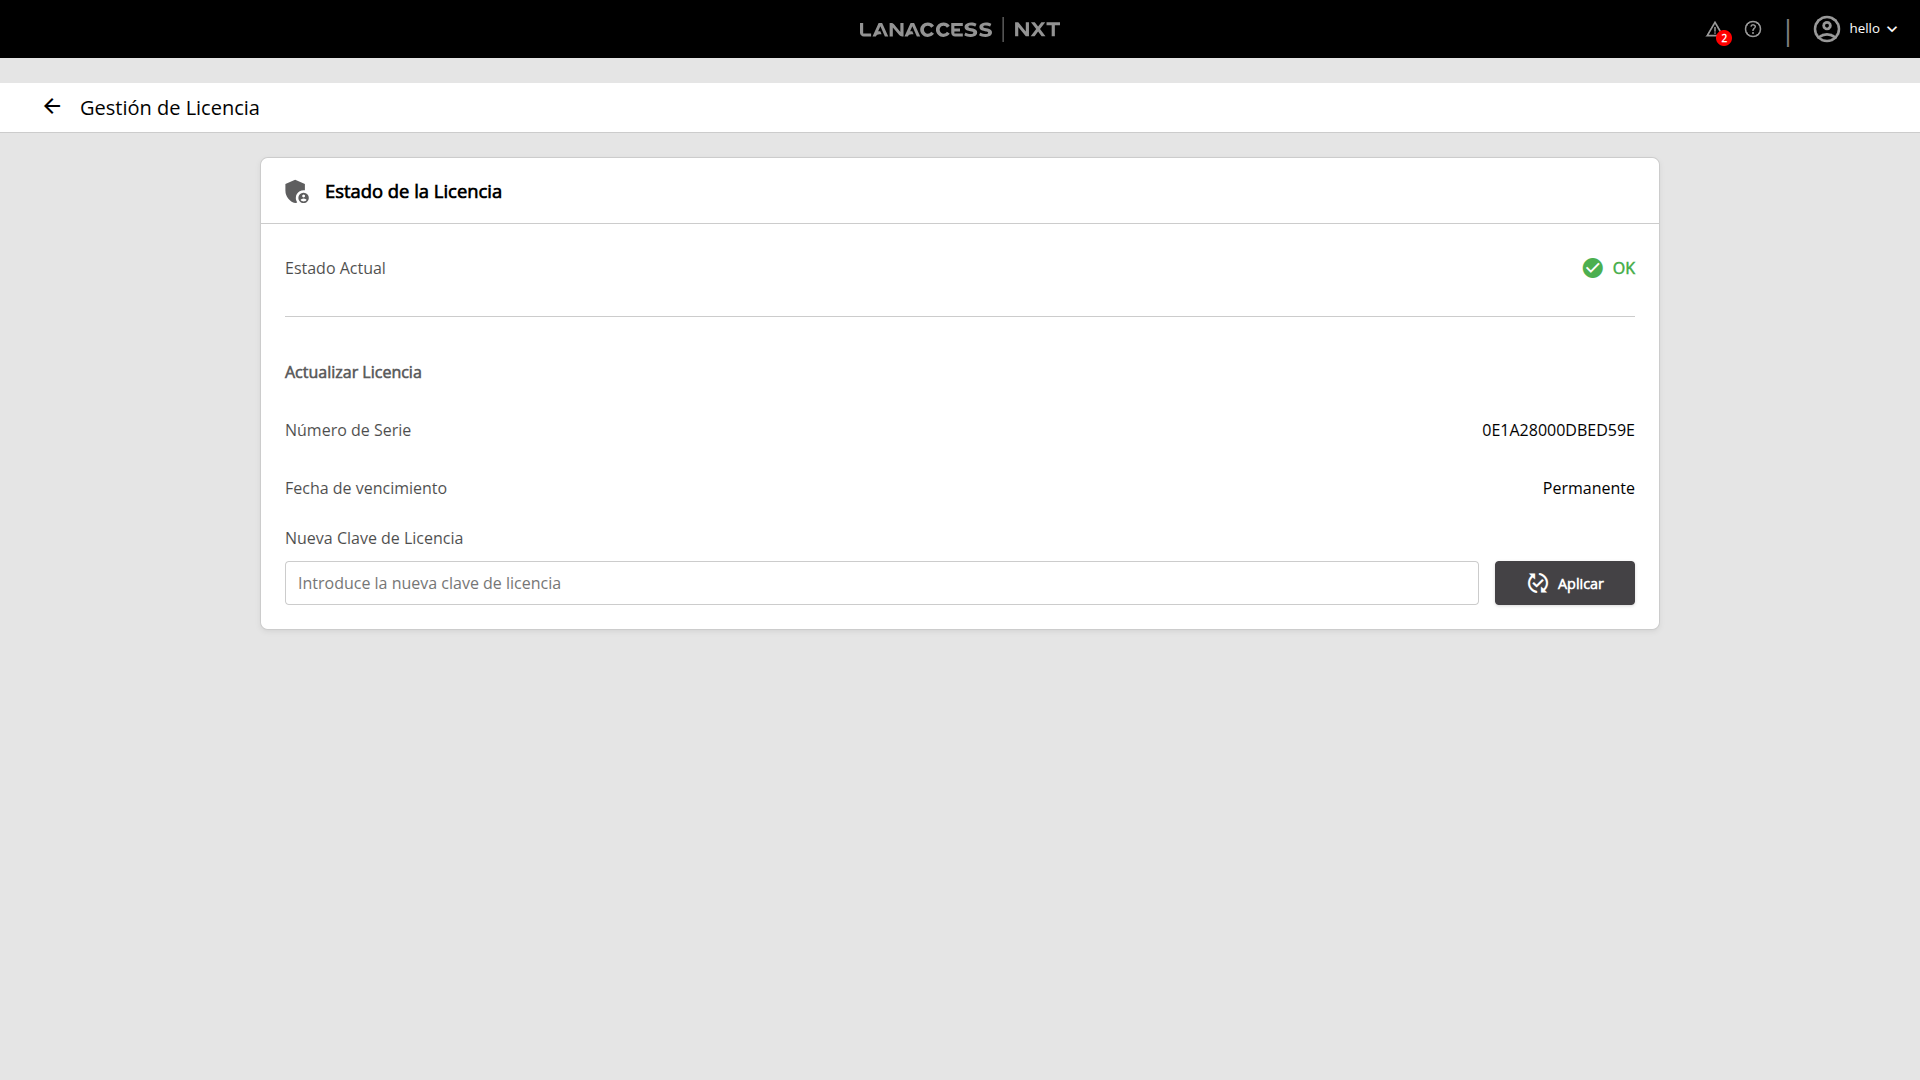
\includegraphics[width=0.95\textwidth]{figures/ui_license.png}
  \caption{Pàgina de gestió de la llicència del sistema.}
  \label{fig:ui_license}
\end{figure}

\subsection{Sistema unificat d'alertes en temps real i canal de notificacions}
Un element clau de la capçalera és la icona de la campana de notificacions (Figura \ref{fig:ui_errors}). La seguretat industrial exigeix que qualsevol anomalia física o lògica (com la pèrdua de senyal d'una càmera, una fallida en un disc d'emmagatzematge o un atac contra el sistema de xarxa) es comuniqui a l'instant.

\begin{figure}[htbp]
  \centering
  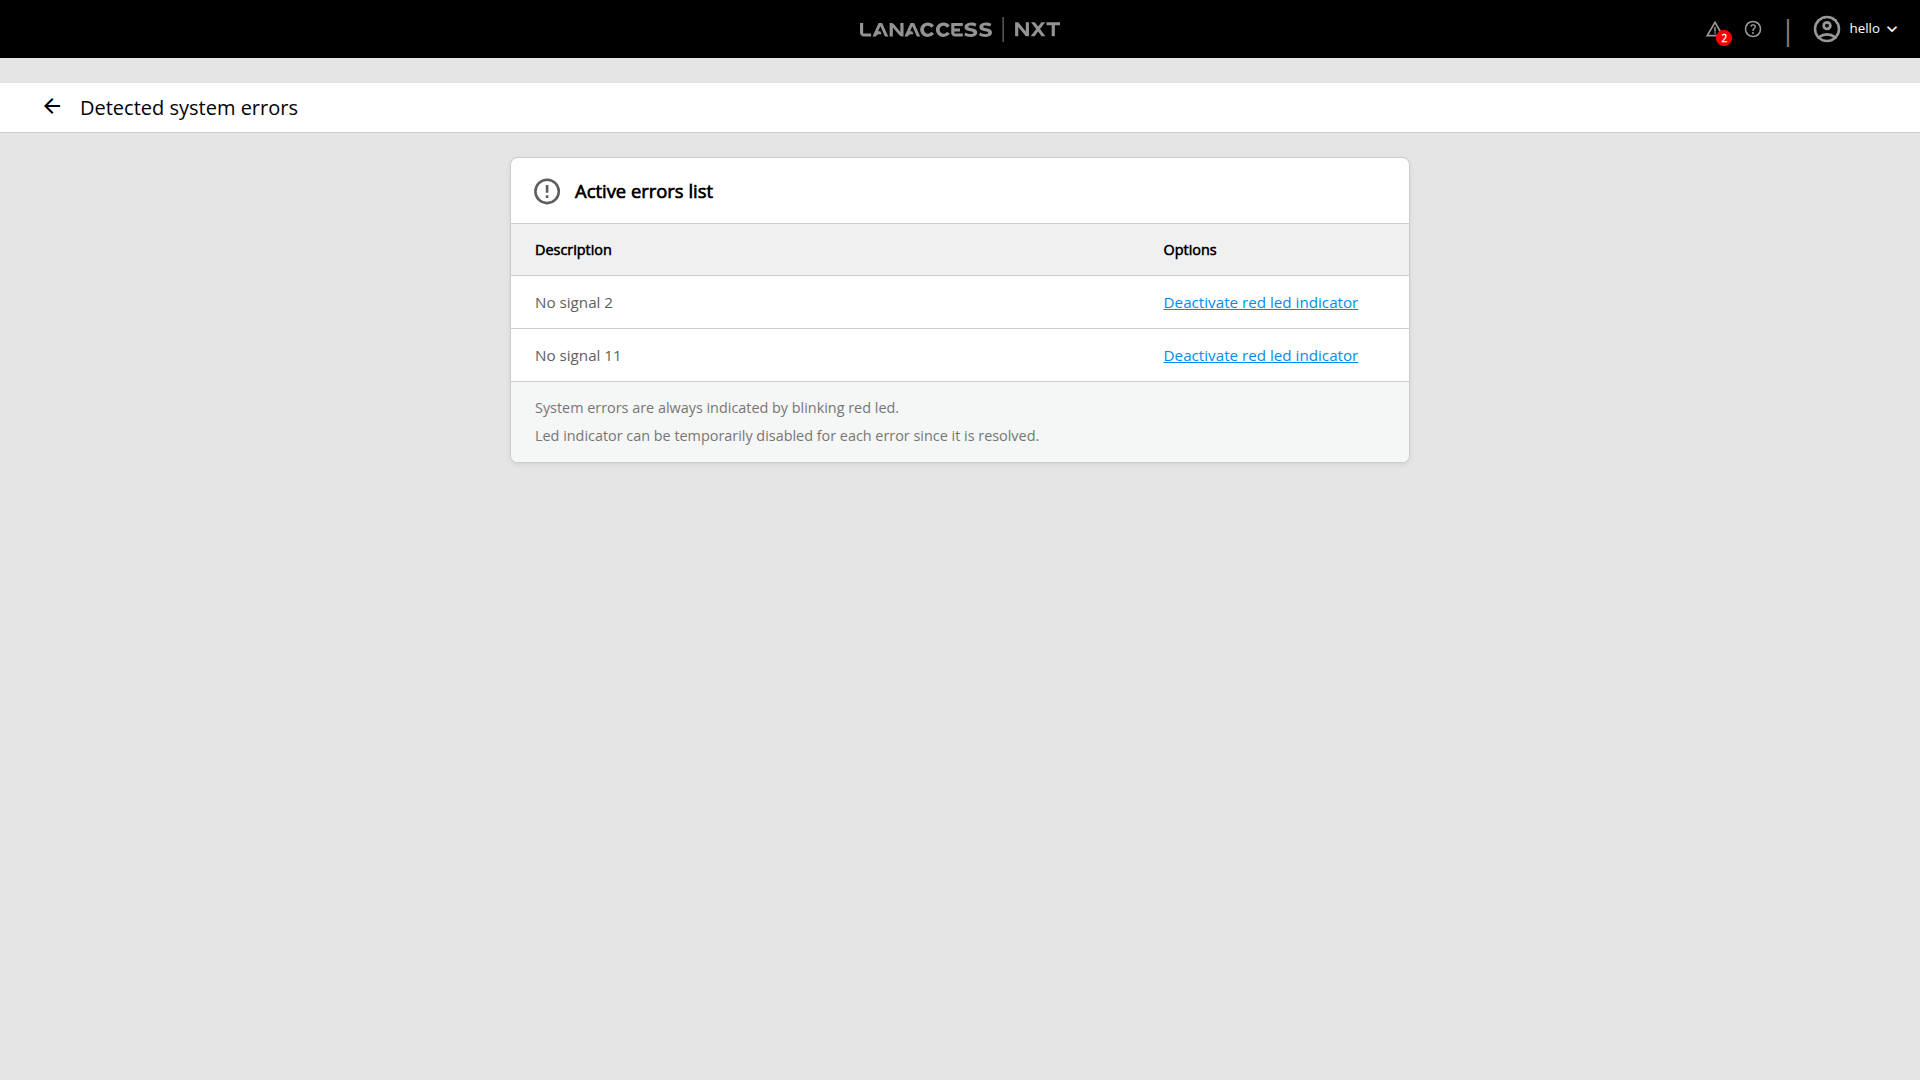
\includegraphics[width=0.95\textwidth]{figures/ui_errors.png}
  \caption{Sistema de notificacions i errors emergents.}
  \label{fig:ui_errors}
\end{figure}

Per aconseguir-ho, l'aplicació implementa una subscripció asíncrona persistent mitjançant el servei de notificacions d'errors unificat (\texttt{AlertService}). Aquest servei manté una connexió constant via WebSocket Segur amb el microservei \textbf{la-core-notifier}. Quan es produeix un esdeveniment a l'NVR, aquest és publicat al bus intern de Linux \textbf{D-Bus}. El servei de notificacions llegeix el senyal, el converteix en un missatge estructurat amb el format \texttt{ERRORS\_NOTIFY} i el transmet immediatament cap al frontend per fer aparèixer un globus de notificació (\textit{badge}) amb el nombre d'alertes pendents sobre la icona de la campana.

Si l'operador fa clic sobre aquest indicador, el sistema el redirigeix cap al panell de diagnòstic d'errors actius (Figura \ref{fig:ui_errors}), on es mostren en detall les fallides actives del sistema, podent interaccionar directament per apagar el senyal de led de l'alarma des de la pantalla web un cop s'ha revisat la incidència.

\section{Configuració del Sistema i Motor Dinàmic (Schema-Driven)}
El disseny de la gestió de configuració de la plataforma \textit{Web Core View} representa una evolució significativa respecte als mètodes tradicionals basats en formularis estàtics o fitxers de configuració dispersos. En lloc de duplicar la lògica de validació al front-end, s'ha implementat una arquitectura de \textbf{Soberania del Backend} (\textit{Backend-Driven Development}), on el gravador NXT actua com a única font de veritat (\textit{Single Source of Truth}).

Dins de l'abast d'aquest projecte, s'ha dissenyat conjuntament amb l'equip d'embedded l'estructura de comunicació de dades i els mecanismes d'hidratació, i s'ha implementat completament en el costat del client el motor d'interpretació dinàmica capaç de transformar metadades JSON en interfícies d'usuari interactives, validades i robustes de manera autònoma.

\subsection{El Model de Validació en Cascada (Cascaded Validation)}
Per evitar l'anomenada \textit{"Configuració Fantasma"} (per exemple, que l'usuari pugui programar gravacions d'una càmera o d'un sensor físicament inexistent), el sistema organitza la informació en un model de validació estructural de tres capes que es complementen de forma jeràrquica:

\begin{enumerate}
  \item \textbf{Capa Teòrica (Esquema):} Defineix les regles abstractes de joc i els límits teòrics del programari de manera declarativa mitjançant fitxers YAML integrats al servei de validació de l'NVR (ex: \textit{"el sistema admet un màxim de 32 entrades"}).
  \item \textbf{Capa Física (Recursos - \texttt{/resources}):} Exposa el maquinari realment connectat o llicenciat en l'equip en temps d'execució mitjançant un conjunt d'APIs REST complementàries (ex: \textit{"aquest equip disposa d'un mòdul físic amb 8 entrades instal·lades"}).
  \item \textbf{Capa Lògica (Dades de Configuració):} Representa l'arbre de configuració real que l'operador decideix aplicar (ex: \textit{"activa la gravació quan l'entrada 3 estigui activa"}).
\end{enumerate}

\begin{figure}[htbp]
  \centering
  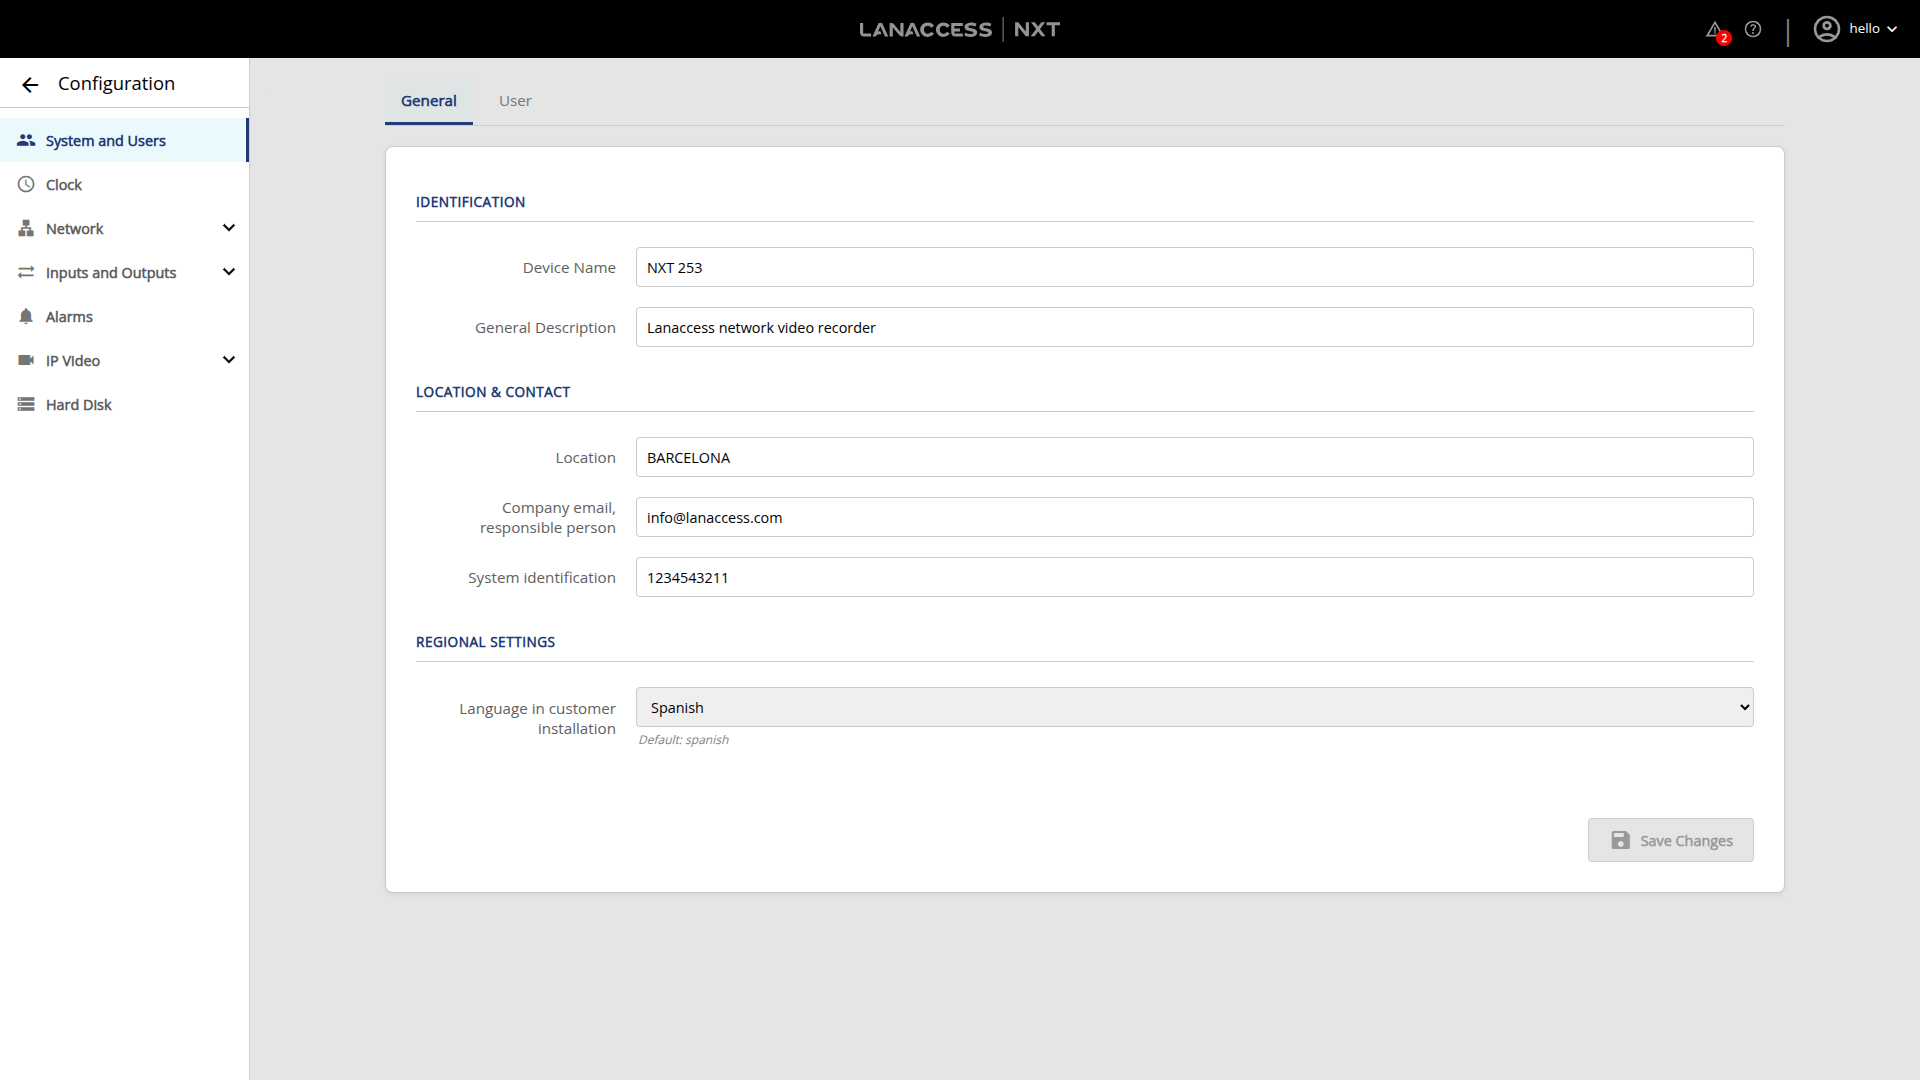
\includegraphics[width=0.95\textwidth]{figures/ui_system1.png}
  \caption{Pantalla de configuració principal del sistema generada dinàmicament.}
  \label{fig:ui_system1}
\end{figure}

Mitjançant aquesta validació en cascada, el client d'Angular consulta de manera proactiva la capa de recursos i l'esquema de dades abans de dibuixar l'interfície. Si l'operador intenta forçar una petició d'escriptura invàlida, el servidor la rebutja immediatament amb un error \texttt{HTTP 422 Unprocessable Entity}.

\subsection{Projecció Virtual i Hidratació de Dades (Merge Logic)}
Internament, per garantir un temps d'accés $O(1)$ i l'eficiència en sistemes de memòria flaix limitats, l'NVR emmagatzema les dades de configuració en un format pla de tipus clau-valor a través del bus del sistema (\texttt{D-Bus}). Tanmateix, per a l'API REST de cara al frontend, el servei \texttt{la-core-legacy} fa una projecció d'aquestes claus per reconstruir en temps real un arbre de dades jeràrquic i tipat en format JSON (Figura \ref{fig:ui_system2}).

\begin{figure}[htbp]
  \centering
  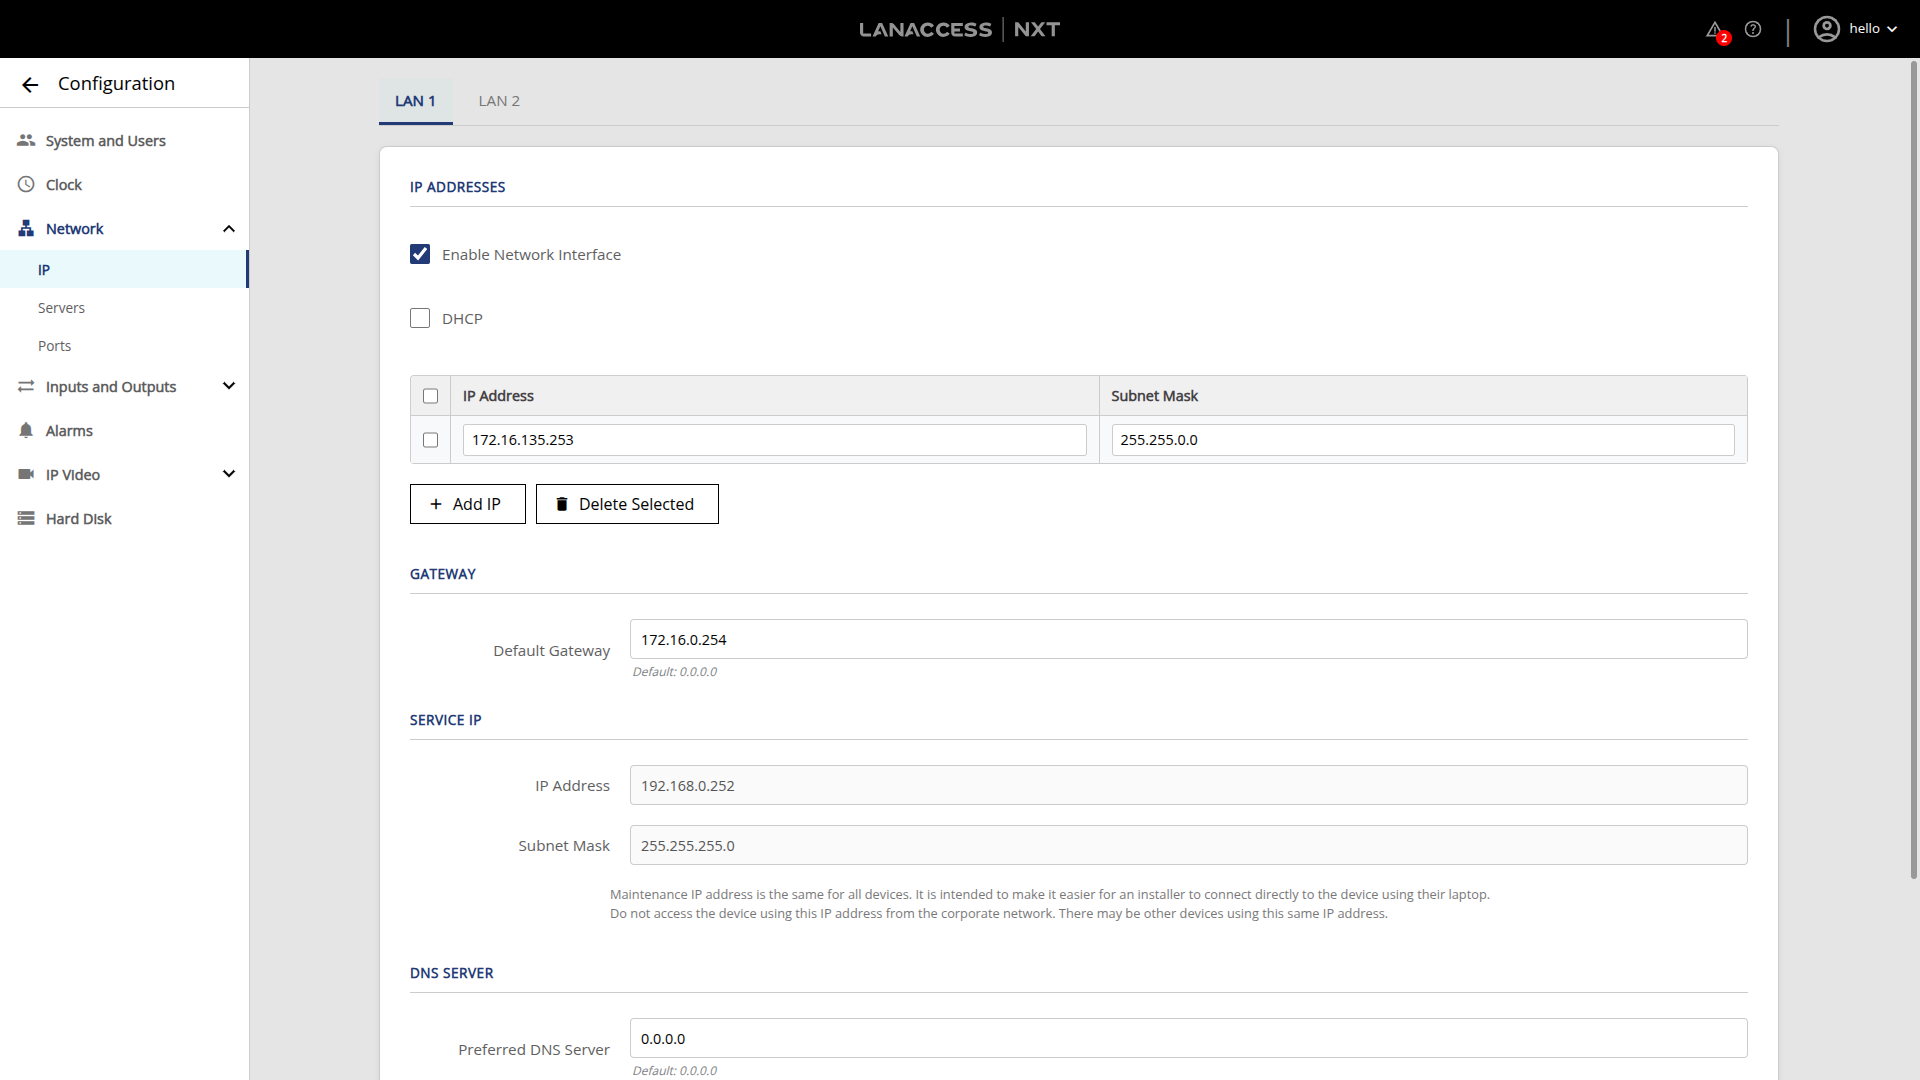
\includegraphics[width=0.95\textwidth]{figures/ui_system2.png}
  \caption{Detall de l'edició de paràmetres de xarxa i interfícies.}
  \label{fig:ui_system2}
\end{figure}

Durant les operacions de lectura (\texttt{GET}), l'API del servidor realitza una operació d'hidratació de dades (\textit{Merge}):
\begin{enumerate}
  \item Carrega de la persistència les dades modificades per l'usuari.
  \item Recorre l'esquema del node en paral·lel. Per a cada propietat que no estigui definida en la persistència, hi injecta automàticament el seu valor per defecte (\texttt{\_default}).
  \item Genera de manera automàtica totes les instàncies lògiques per a col·leccions fixes definides pel maquinari (ex: cam01 a cam16), evitant que l'aplicació Angular hagi d'omplir buits amb lògica condicional defensiva.
\end{enumerate}

\subsection{Motor Dinàmic del Frontend (Schema-Driven Rendering)}
El client web actua com un intèrpret asíncron de les definicions d'esquema exposades per l'endpoint \texttt{/device-service/properties/schema}. El component dinàmic \texttt{ConfigInputComponent} rep la definició i renderitza de forma autònoma el component de presentació equivalent, utilitzant un flux recursiu basat en el tipus semàntic de la propietat d'esquema, tal com s'il·lustra a la Figura \ref{fig:ui_system3}:

\begin{itemize}
  \item \texttt{\_type: "boolean"}: Es renderitza mitjançant un commutador (\texttt{ToggleComponent}).
  \item \texttt{\_type: "integer" / "numeric"}: Si té restriccions de màxims i mínims, genera un element lliscant (\texttt{SliderComponent}) o un camp numèric normalitzat.
  \item \texttt{\_type: "list"}: Genera un selector de llista desitjada (\texttt{SelectComponent}) basat en els elements del vector \texttt{\_allowedValues}.
  \item \texttt{\_type: "flag"}: Configura una màscara de selecció múltiple.
  \item \texttt{\_type: "resource\_list" / "resource\_flag"}: Modifica la llista d'opcions connectant dinàmicament el selector amb les instàncies del maquinari real obtingut prèviament d'una consulta a \texttt{/resources}.
\end{itemize}

\begin{figure}[htbp]
  \centering
  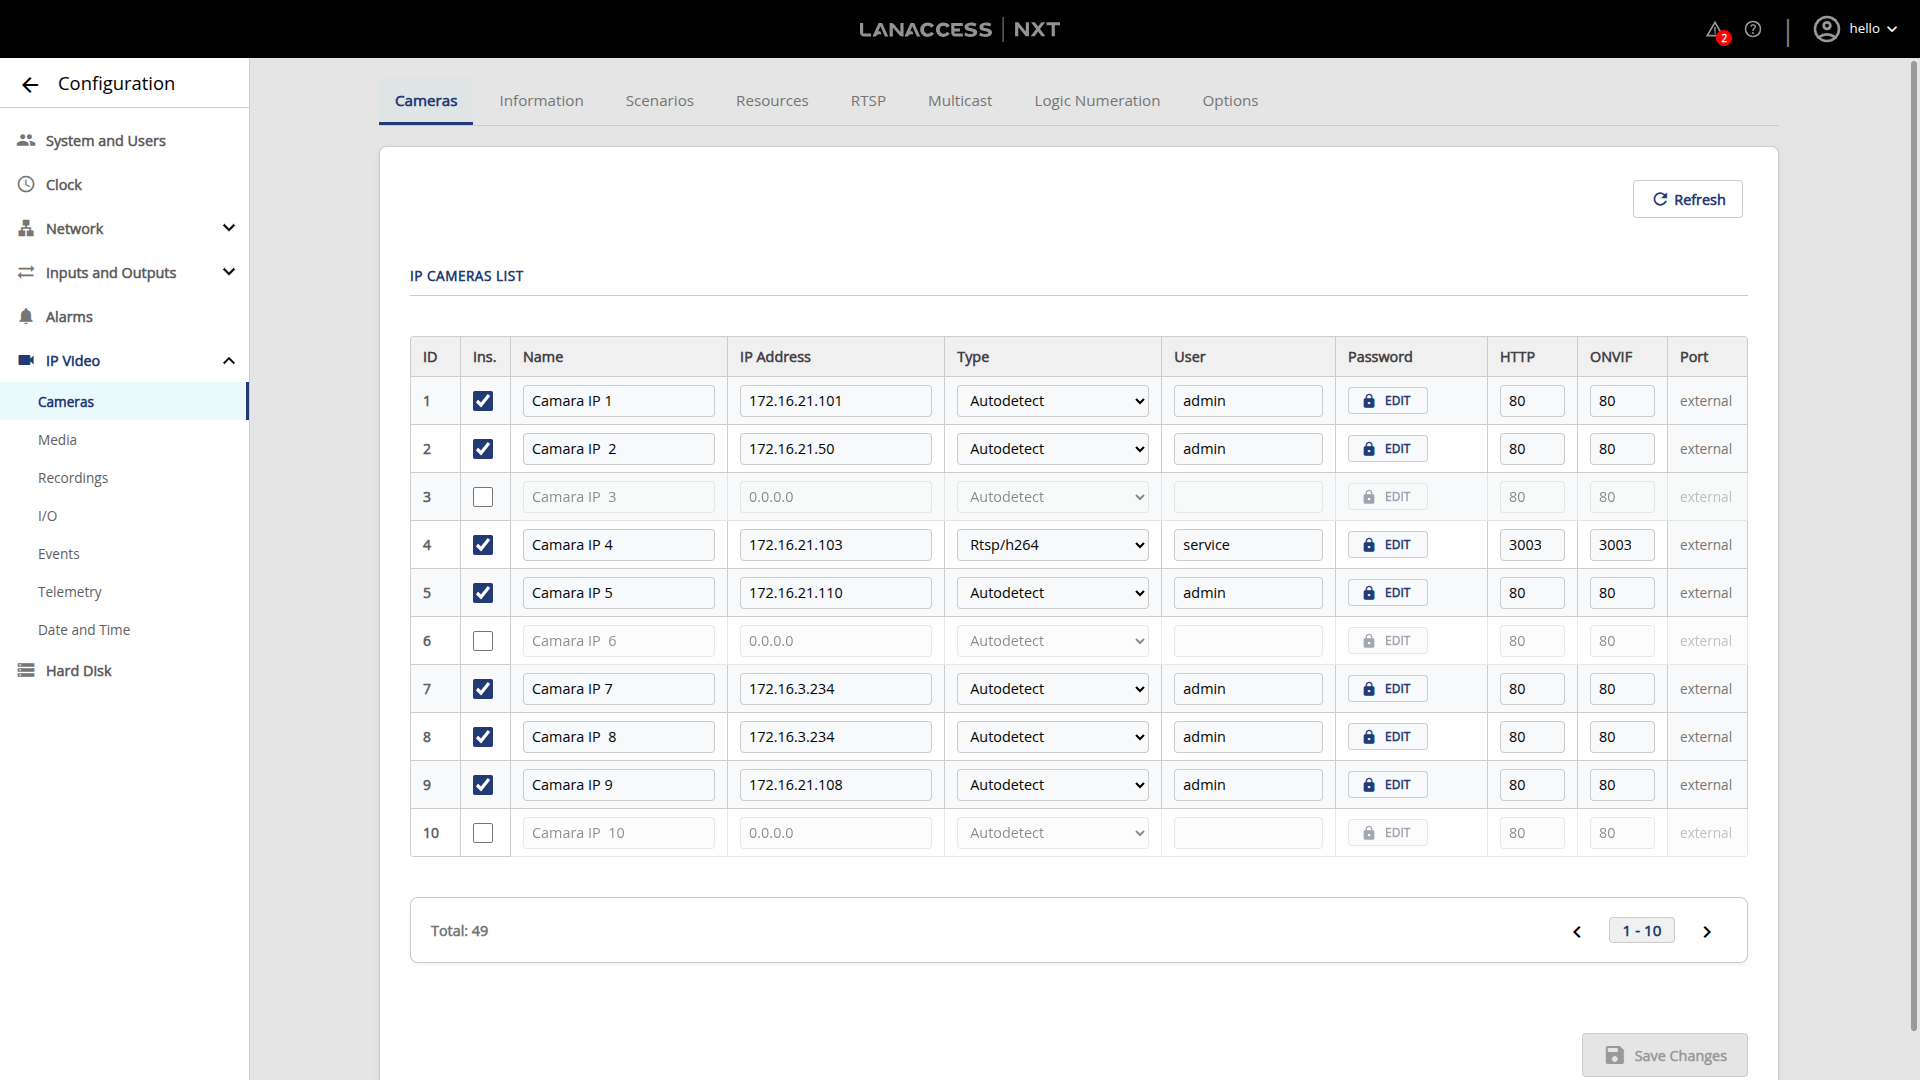
\includegraphics[width=0.95\textwidth]{figures/ui_system3.png}
  \caption{Desplegables (\textit{selects}) i botons commutadors (\textit{toggles}).}
  \label{fig:ui_system3}
\end{figure}

\subsection{Validació Dinàmica de Tipus i Formats amb Signals}
Per garantir la integritat de les dades del costat de client i guiar l'operador abans de fer l'enviament, s'ha programat una variable reactiva calculada (\textit{computed signal}) anomenada \texttt{computedValidationError}. Aquesta avalua de forma instantània el valor escrit contra les regles declaratives de l'esquema:

\begin{lstlisting}[language=JavaScript, caption={Lògica de validació dinàmica amb \textit{Signals} i \textit{Regex} a ConfigInputComponent.}]
computedValidationError = computed(() => {
  const value = this.inputValue();
  const def = this.fieldDef();
  if (!def) return null;

  // 1. Validacio de patrons d'expressio regular (ex: IP, Mascara, Domain)
  if (def._regex) {
    const rx = new RegExp(def._regex);
    if (!rx.test(String(value))) {
      return def._description || 'Format invalid';
    }
  }

  // 2. Validacio de limits numerics de rang
  if (def._type === 'integer' || def._type === 'numeric' || def._type === 'decimal') {
    const minVal = def._min !== undefined ? def._min : def._minValue;
    const maxVal = def._max !== undefined ? def._max : def._maxValue;
    if (minVal !== undefined && value < minVal) return `Minim: ${minVal}`;
    if (maxVal !== undefined && value > maxVal) return `Maxim: ${maxVal}`;
  }

  // 3. Validacio de longituds de text
  if (def._type === 'string') {
    if (def._minLength && String(value).length < def._minLength) {
      return `Minim ${def._minLength} caracters`;
    }
    if (def._maxLength && String(value).length > def._maxLength) {
      return `Maxim ${def._maxLength} caracters`;
    }
  }
  return null;
});
\end{lstlisting}

\subsection{Gestió de Centineles i Valors Buits}
Un repte arquitectònic clau d'aquest model híbrido (dades jeràrquiques sobre disc pla clau-valor) és el tractament dels camps buits. En els sistemes de dades plans, enviar una cadena buida (\texttt{""}) s'interpreta normalment com una ordre per esborrar física i completament la clau de la memòria d'emmagatzematge.

Tanmateix, a la lògica de negoci de l'NVR, una cadena buida pot ser una opció de configuració voluntària i explícita (per exemple, decidir que una alarma no realitzi cap acció, eliminant les accions per defecte \texttt{"record+relay"}). Si el servidor esborrés la clau física del disc, en el següent procés d'hidratació s'injectaria erròniament el valor per defecte del programari.

Per resoldre aquest problema, s'ha implementat el centinela de dades buides \texttt{\_\_is\_empty\_}. Quan l'operador neteja un camp a l'aplicació web, l'API REST de backend intercepta la petició abans de la seva persistència, detecta la intenció de buidar la dada i escriu la cadena \texttt{\_\_is\_empty\_} sobre la clau corresponent del NVR. Durant els fluxos de lectura, el motor tradueix el centinela un altre cop a un \texttt{""} real, abstenint-se d'injectar-hi la propietat per defecte.

\subsection{Control de Concurrència i Bloqueig Pesimista (Locking)}
Per assegurar l'atominicitat de les modificacions i prevenir col·lisions d'escriptura en entorns multi-administrador o multiclient (incloses diferents pestanyes del mateix navegador), s'ha codificat un algorisme de \textbf{bloqueig pesimista} (\textit{Pessimistic Locking}) recolzat pel paràmetre \texttt{seed} de sessió.

Abans d'entrar en mode edició, l'usuari ha de sol·licitar l'adquisició del cadenat. El frontend genera un identificador aleatori (\textit{seed}) que s'emmagatzema a l'espai d'execució d'aquesta pestanya (\texttt{sessionStorage}). Es demana el bloqueig al servei \texttt{la-core-legacy}:

\begin{lstlisting}[language=json, caption={Resposta exitosa de l'API de bloqueig (200 OK).}]
{
  "token": "aVQ3wjNZ5QIXNAGjhfGgYdpFDWoHsJW5",
  "expiresIn": 30,
  "path": "config"
}
\end{lstlisting}

Un cop adquirit, es dispara des d' Angular un cicle d'actualització o batec de cor (\textit{heartbeat}) que manté el cadenat actiu cada 15 segons. Per evitar que la reactivitat d'aquest temporitzador provoqui avaluacions d'estat innecessàries de l'arbre de components del navegador, s'ha configurat per executar-se fora del context de detecció de canvis de \texttt{Zone.js}:

\begin{lstlisting}[language=JavaScript, caption={Optimització del cicle de vida de Zone.js per a la renovació del cadenat.}]
private scheduleRenewal(ms: number) {
  this.stopRenewal();
  this.zone.runOutsideAngular(() => {
    this.renewalTimer = setTimeout(() => {
      this.zone.run(() => this.acquireLock());
    }, ms);
  });
}
\end{lstlisting}

\begin{figure}[htbp]
  \centering
  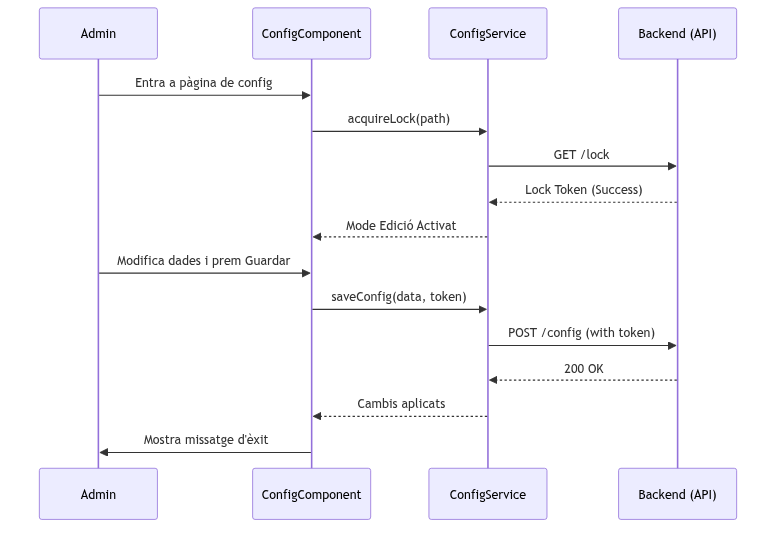
\includegraphics[width=0.9\textwidth]{figures/seq_config_lock.png}
  \caption{Diagrama de seqüència del procés d'adquisició i alliberament de Lock de configuració.}
  \label{fig:seq_config_lock}
  \small Font: Elaboració pròpia.
\end{figure}

Si el recurs està ocupat, el servidor respon amb un codi \texttt{HTTP 409 Conflict} aportant el nom de l'usuari i la IP que té el bloqueig, obligant l'aplicació Angular a bloquejar la vista actual com a "Només lectura" de forma instantània (Figura \ref{fig:seq_config_lock}).

\subsection{Detecció de Deltes i Gestió de Reinicis}
En prémer el botó de desar, en lloc d'enviar tot l'arbre de configuració (el que saturaria el canal d'escriptura i el maquinari del gravador), s'executa l'algorisme recursiu de diferències programat en el frontend (\texttt{getObjectDelta}), comparant l'estat actual contra l'estat inicial original. Les modificacions s'envien mitjançant peticions parcials \texttt{PATCH}:

\begin{lstlisting}[language=JavaScript, caption={Algorisme recursiu de detecció de Deltes per a l'optimització de payloads amb normalització de primitius.}]
export function getObjectDelta(current: any, original: any, path: string = ''): any {
  const normalize = (val: any) => {
    if (val === 'true') return true;
    if (val === 'false') return false;
    return val;
  };

  const normCurrent = normalize(current);
  const normOriginal = normalize(original);

  if (normCurrent === normOriginal) return undefined;
  if (typeof normCurrent !== 'object' || normCurrent === null) return normCurrent;

  const delta: any = {};
  let hasChanges = false;

  for (const key in normCurrent) {
    if (key.startsWith('_')) continue; // Ignora camps estructurals de l'esquema
    
    const currentVal = normCurrent[key];
    const originalVal = normOriginal ? normOriginal[key] : undefined;

    const diff = getObjectDelta(currentVal, originalVal, `${path}.${key}`);
    
    // Evita la propagacio de sub-objectes buits sense canvis reals
    if (diff !== undefined && (typeof diff !== 'object' || Object.keys(diff).length > 0)) {
      delta[key] = diff;
      hasChanges = true;
    }
  }
  
  return hasChanges ? delta : undefined;
}
\end{lstlisting}

Un aspecte de rendiment crític gestionat pel backend és la detecció automàtica de si el canvi d'un d'aquests paràmetres requereix reiniciar l'NVR per aplicar-se (marcat amb la propietat \texttt{\_rebootRequired: true} dins del seu esquema de definició YAML).

Quan s'aplica l'escriptura de dades, el validador del backend avalua si qualsevol camp de la delta conté aquesta bandera. Si és així, el servidor estableix automàticament un indicador global de "Reinicio pendent" i injecta de manera asíncrona la capçalera personalitzada \texttt{X-Reboot-Required: true} a la resposta HTTP de l'API. L'interceptor d'Angular llegeix la capçalera i actualitza l'estat de les vistes, de manera que el frontend sap de forma dinàmica i unificada quan avisar l'operador, sense necessitat de duplicar aquesta lògica de negoci complexa en el codi de la interfície de client.

\section{Assistents de Configuració (Wizards)}
El sistema també disposa d'assistents pas a pas (\textit{Wizards}) per facilitar la posada en marxa ràpida de l'equip a operadors sense coneixements tècnics avançats. S'ha adaptat completament l'estètica CSS de l'eina \textit{legacy} per adequar-la al disseny modern i reactiu de la nova aplicació, guiant l'usuari en la detecció automàtica de càmeres IP a la xarxa local de forma interactiva i assistida.

\section{Eina de Xarxa: Web Proxy}
Atès que, per motius de seguretat, algunes càmeres IP estan connectades a ports aïllats del gravador (creant una subxarxa no accessible des de l'exterior), l'aplicació integra l'eina de \textit{Web Proxy}.

\begin{figure}[htbp]
  \centering
  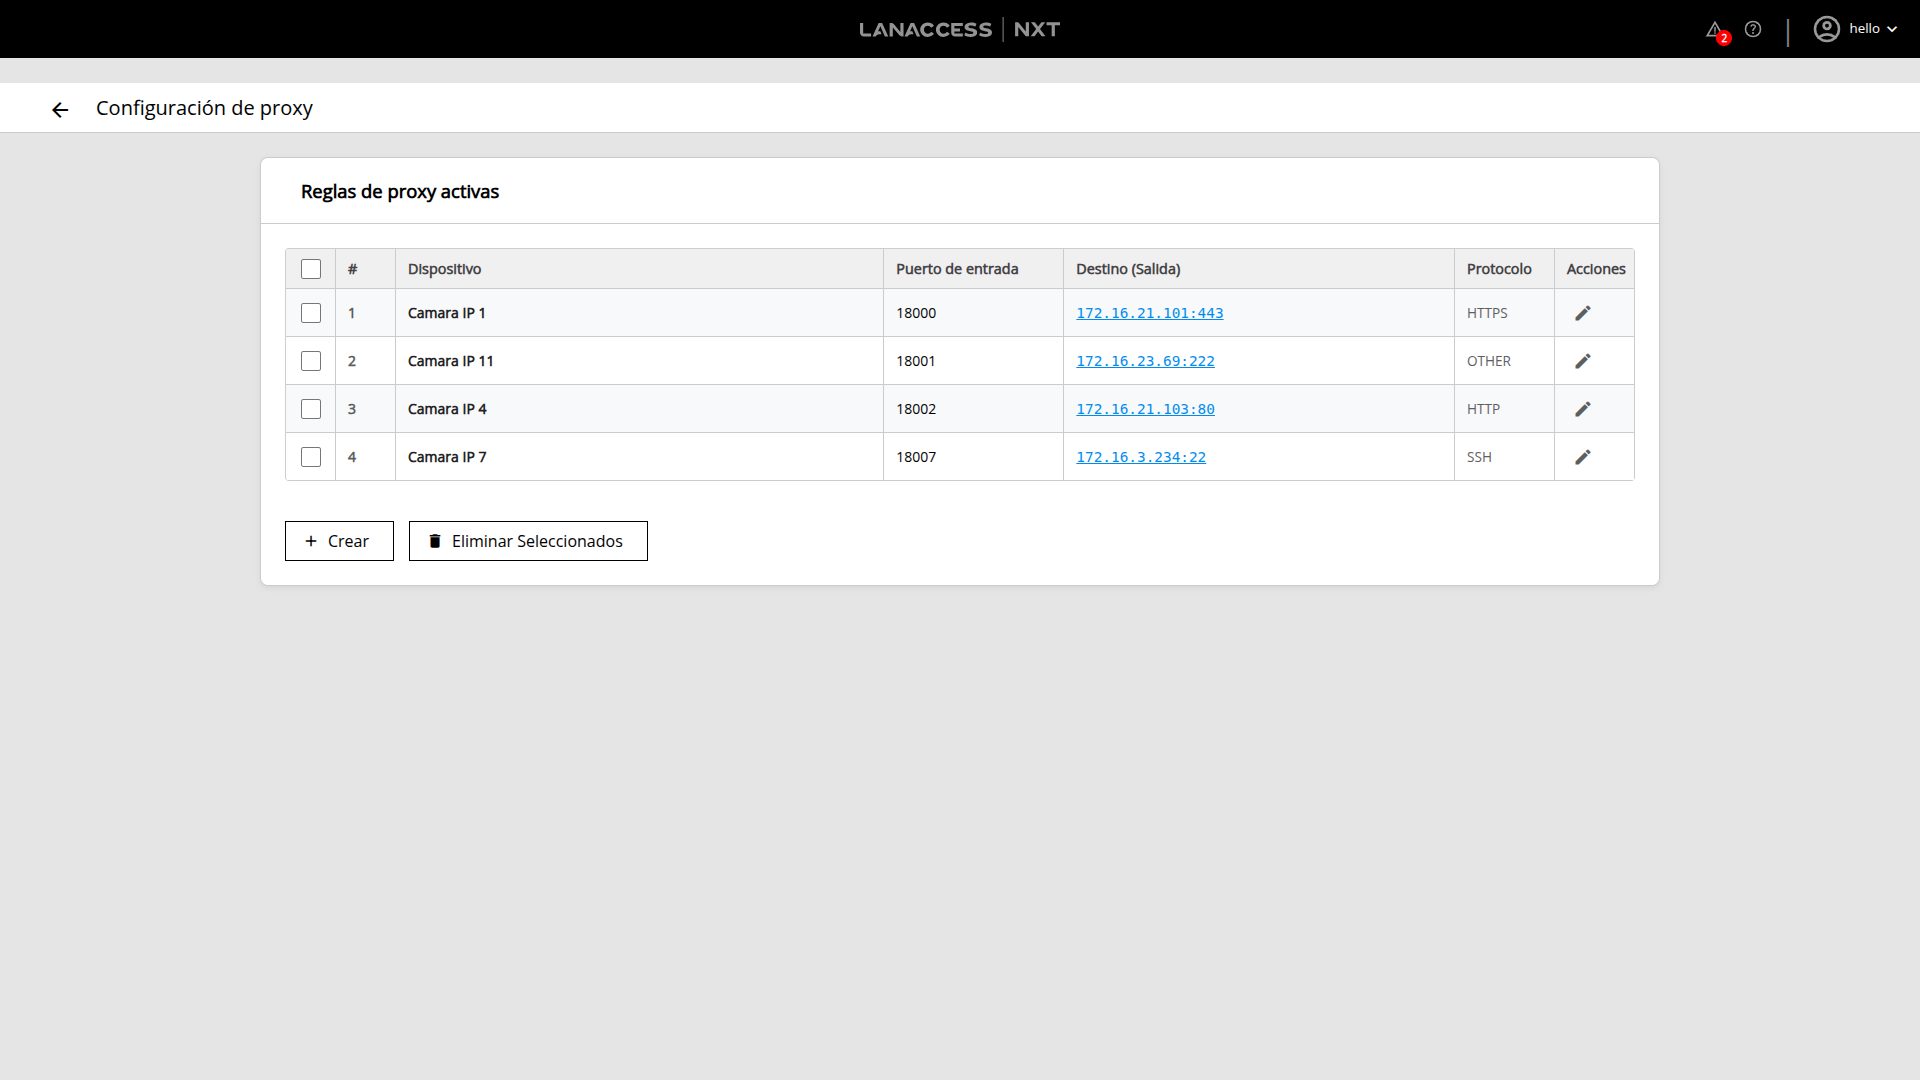
\includegraphics[width=0.95\textwidth]{figures/ui_proxy.png}
  \caption{Eina de Web Proxy per a l'accés a càmeres aïllades en subxarxes internes.}
  \label{fig:ui_proxy}
\end{figure}

Mitjançant aquesta pantalla senzilla (Figura \ref{fig:ui_proxy}), l'administrador pot introduir la IP local de la càmera i el port. El \textit{frontend} es comunica amb \textbf{la-core-legacy} per ordenar la creació d'un túnel invers intern, permetent l'accés al portal web natiu de la càmera des de dins de l'aplicació \textit{Web Core View}.

\section{Visualització Multimèdia en Directe i Arquitectura del Servidor de Vídeo}
La visualització de vídeo en directe representa el component més crític de l'operativa de seguretat diària. Per aconseguir un flux de streaming d'alta fidelitat i eliminar l'ús de connectors externs o codi propietari del costat de client, s'ha implementat una arquitectura híbrida de vídeo integrada al sistema operatiu embedded del gravador NXT, utilitzant el protocol de comunicació estàndard \textbf{WebRTC} com a canal de transport principal i \textbf{HLS} (\textit{HTTP Live Streaming}) com a mètode de contingència o \textit{fallback}.

\begin{figure}[htbp]
  \centering
  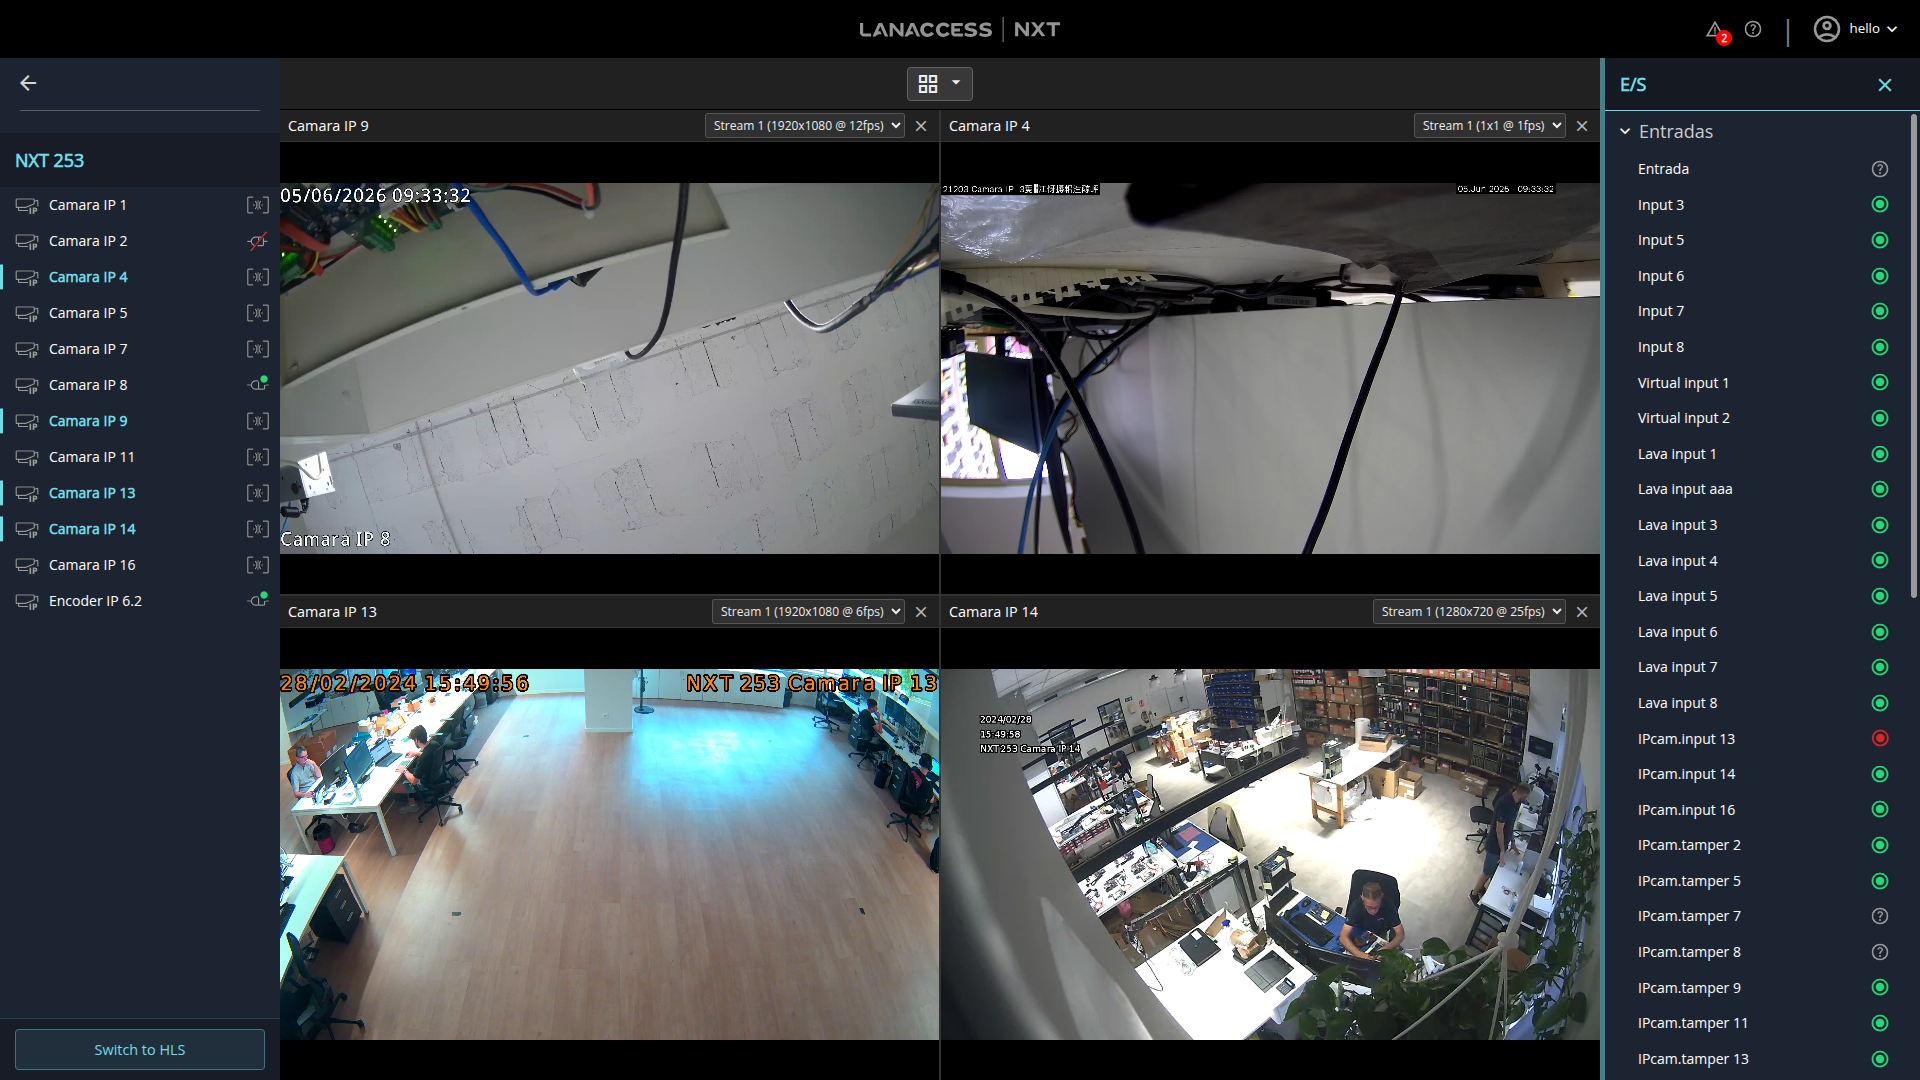
\includegraphics[width=0.95\textwidth]{figures/ui_cameras.png}
  \caption{Mosaic de visualització de vídeo en directe.}
  \label{fig:ui_cameras}
\end{figure}

A nivell de maquinari del gravador, l'arquitectura de transmissió de vídeo es divideix en dues capes diferenciades coordinades pel microservei \textbf{la-video-engine}:

\begin{enumerate}
  \item \textbf{Motor d'Adquisició i Processat (GStreamer):} Per a cadascuna de les càmeres IP físiques instal·lades, l'NVR inicialitza un pipeline de dades basat en el framework multimèdia industrial \textbf{GStreamer}. Aquest pipeline s'encarrega d'obrir el flux \textit{RTSP} natiu de la càmera, extreure'n els paquets de vídeo, normalitzar el senyal de rellotge i decodificar de forma accelerada per maquinari part dels fotogrames crítics per a la generació de metadades analítiques.
  \item \textbf{Servidor de Mitjans WebRTC (MediaMTX):} Els fotogrames de vídeo capturats i empaquetats per GStreamer es canalitzen internament en un pipeline d'escriptura cap al servidor multimèdia d'alt rendiment \textbf{MediaMTX} (actuant com a servidor centralitzat de WebRTC i WHEP). Aquest servei gestiona la negociació SDP (\textit{Session Description Protocol}), el xifratge de paquets SRTP sobre transport UDP, i serveix el vídeo amb una latència punta a punta inferior a 300 ms natius en qualsevol navegador web actual, recolzant-se en la targeta gràfica (GPU) del dispositiu del client per a la descodificació fina.
\end{enumerate}

Davant de xarxes corporatives on el trànsit UDP pugui estar completament bloquejat pel tallafocs de l'empresa (la qual cosa impedeix establir el canal de vídeo per defecte d'ICE), el sistema activa de forma transparent un mecanisme de degradació de servei cap a \textbf{HLS} (\textit{HTTP Live Streaming}). Aquesta via de redundància s'estableix a través del proxy invers NGINX mitjançant el port de comunicació de dades estàndard (TCP 443), assegurant la visualització contínua i sense talls del senyal a costa d'un petit increment de la latència que no excedeix el límit operatiu.

\subsection{La Interfície de Càmeres i el Disseny de Mosaic}
A la pàgina de Càmeres (Figura \ref{fig:ui_cameras}), l'operador disposa de controladors visuals per commutar la distribució de la graella multimèdia (\textit{layouts} de tipus $1\times1$, $2\times2$ i $4\times4$). Cadascuna de les cel·les que formen aquest mosaic és un component d'Angular unificat i encapsulat anomenat \texttt{GridVideoPlayerComponent}, el qual gestiona el cicle de vida del seu propi reproductor independent.

La interfície implementa una lògica d'arrossegar i deixar anar (\textit{Drag and Drop}) nativa integrada amb la llista lateral de càmeres del panell esquerre. L'usuari pot arrossegar qualsevol càmera cap a una cel·la del mosaic. Aquesta acció de drop recupera la identitat del dispositiu d'entrada, demana el seu mètode d'accessibilitat i demana de forma dinàmica la càrrega del flux, seguint el cicle d'activitat descrit a la Figura \ref{fig:activity_video_connection}.

\begin{figure}[htbp]
  \centering
  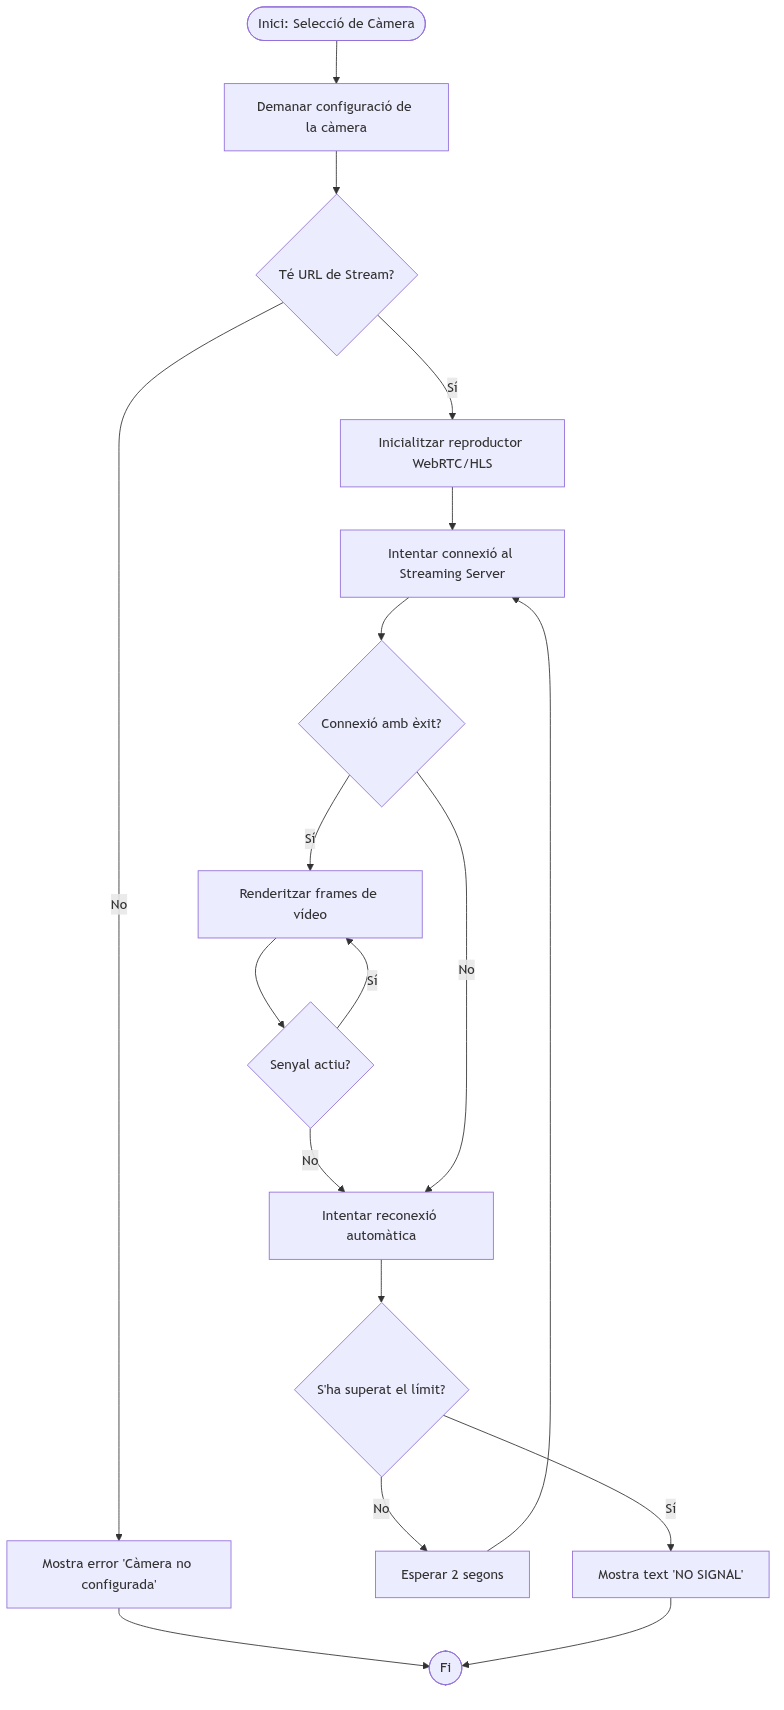
\includegraphics[width=0.65\textwidth]{figures/activity_video_connection.png}
  \caption{Diagrama d'activitat de la lògica de connexió i reconnexió de vídeo.}
  \label{fig:activity_video_connection}
\end{figure}

\subsection{Negociació SDP i Establiment del Canal de Streaming}
Si la xarxa del client disposa dels canals lliures de comunicació, el frontend i el servidor MediaMTX inicien la negociació SDP mitjançant el protocol d'egress de mitjans unificat \textbf{WHEP} (\textit{WebRTC HTTP Egress Protocol}):

\begin{lstlisting}[language=JavaScript, caption={Lògica simplificada de la PeerConnection per WebRTC.}]
async startStreaming(cameraId: string) {
  const pc = new RTCPeerConnection(this.config);
  
  // Generacio de l'oferta local de presentacio
  const offer = await pc.createOffer();
  await pc.setLocalDescription(offer);
  
  // Enviament al servidor MediaMTX a traves de la-video-engine
  this.videoService.sendOffer(cameraId, offer).subscribe(answer => {
    // Aplicacio de la resposta del servidor (Answer) per establir el canal
    pc.setRemoteDescription(answer);
  });
}
\end{lstlisting}

Aquest intercanvi de metadades descrit en el diagrama de seqüència de la Figura \ref{fig:seq_video_streaming} defineix quins còdecs d'escriptura (H.264 o H.265) i resolucions utilitzarà l'enllaç abans d'iniciar el transport segur dels paquets sobre canals UDP.

\begin{figure}[htbp]
  \centering
  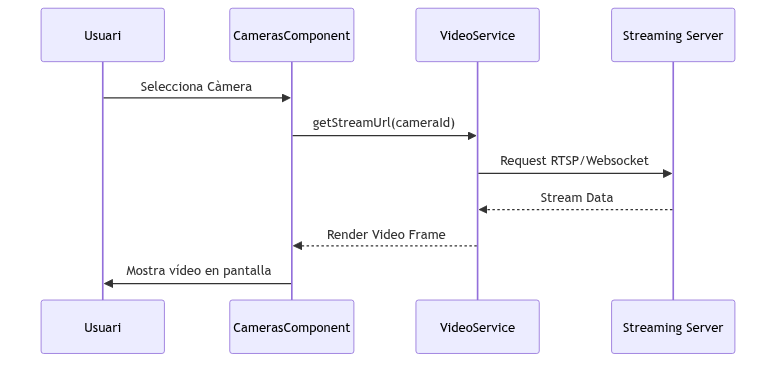
\includegraphics[width=0.85\textwidth]{figures/seq_video_streaming.png}
  \caption{Diagrama de seqüència de l'establiment de streaming de vídeo (SDP).}
  \label{fig:seq_video_streaming}
\end{figure}

\subsection{Orquestració de Vídeo amb el Patró Strategy}
Per estructurar el reproductor multifluj, s'ha aplicat el patró de disseny de programari \textbf{Strategy} d'Angular. Aquest disseny desacobla completament el component visual de la graella de les APIs i llibreries de tercers implicades en la descodificació. Es defineix la interfície comuna \texttt{StreamingStrategy} que actua com a contracte o interfície abstracta unificada:

\begin{lstlisting}[language=JavaScript, caption={Interfície comuna \texttt{StreamingStrategy}.}]
export interface StreamingStrategy {
  connectionState: Signal<'connecting' | 'connected' | 'error' | 'idle'>;
  errorMessage: Signal<string | null>;
  startStream(videoElement: HTMLVideoElement, cameraName: string): Promise<void>;
  closeStream(): void;
}
\end{lstlisting}

Un \textit{InjectionToken} personalitzat allotjat a la declaració del component injecta dinàmicament l'estratègia correcta (ja sigui el servei WebRTC o la via de redundància HLS) en funció de les capacitats obtingudes del mètode de streaming triat:

\begin{lstlisting}[language=JavaScript, caption={Proveïdor per a la injecció dinàmica de l'estratègia de vídeo al \texttt{GridVideoPlayerComponent}.}]
export const STREAMING_STRATEGY_TOKEN = new InjectionToken<StreamingStrategy>('StreamingStrategy');

@Component({
  selector: 'app-grid-video-player',
  // ...
  providers: [
    {
      provide: STREAMING_STRATEGY_TOKEN,
      useFactory: () => {
        const method = getStreamingMethod();
        return method === 'hls' ? inject(HlsService) : inject(WebRTCService);
      }
    }
  ]
})
\end{lstlisting}

Gràcies a l'arquitectura del patró de disseny *Strategy*, el component de visualització és capaç d'intercanviar protocols de transport de manera totalment asíncrona i transparent per a l'usuari en temps de d'execució.

\subsection{Gestió en Temps Real de les Entrades i Sortides Digitals (I/O)}
De forma complementària al panell de visualització de les càmeres de seguretat, la vista principal disposa d'un panell lateral interactiu de control d'entrades i sortides lògiques (I/O), anomenat \texttt{CamerasIoPanelComponent}. Aquest panell permet realitzar la supervisió d'accessos en temps real i accionar relés de manera manual des d'una interfície unificada.

La reactivitat dels indicadors visuals es manté gràcies a l'obertura d'un canal d'esdeveniments unificat via WebSocket d'alta velocitat connectat directament al microservei \textbf{la-core-notifier}. L'arquitectura utilitza l'esquema següent per a la gestió interactiva d'aquests recursos:

\begin{itemize}
  \item \textbf{Supervisió de Canvis (Estat d'Entrada):} El servei escolta el flux del canal i rep el tipus d'esdeveniment \texttt{IO\_NOTIFY}. En rebre la dada, actualitza a l'instant el mètode reactiu de la llista de sensors digital, fent canviar el color de l'indicador del DOM (verd per a \textit{deactivated/idle}, vermell per a \textit{activated/on}).
  \item \textbf{Activació Manual (Estat de Sortida):} Si el perfil de l'operador disposa de permisos de control d'I/O de tipus d'escriptura actius, pot realitzar un doble clic sobre qualsevol de les sortides lògiques configurades, o obrir el menú contextual a través de la icona corresponent.
  \item \textbf{Viatge de Dades:} Aquesta interacció de client desencadena de forma immediata una petició d'escriptura POST unificada cap al servei \textbf{la-core-legacy} sota la ruta \texttt{output-status-set.cgi}. El backend llegeix el camí, valida la intenció i commuta l'estat del relé físic a nivell del maquinari. Un cop realitzat el canvi de sortida, l'NVR llança el senyal de variació a D-Bus, que es propaga a tots els clients connectats a través de WebSocket unificat, garantint la consistència immediata de l'estat global del sistema.
\end{itemize}

\section{Reproducció de Gravacions Històriques i Arquitectura de Playback}
La consulta i reproducció de gravacions passades és un pilar indispensable de l'operativa de seguretat, ja que permet als operadors analitzar i extreure evidències gràfiques d'incidents ja ocorreguts. En el marc d'aquest projecte, s'ha dissenyat i desenvolupat íntegrament tant la capa lògica de negoci del \textit{backend} (l'arquitectura de segmentació, l'indexador de franges de temps i el servidor de mitjans d'HLS integrats al servei \textbf{la-video-engine}) com la interfície interactiva de control del client a Angular 19 (mòdul de \textit{Playback}).

\begin{figure}[htbp]
  \centering
  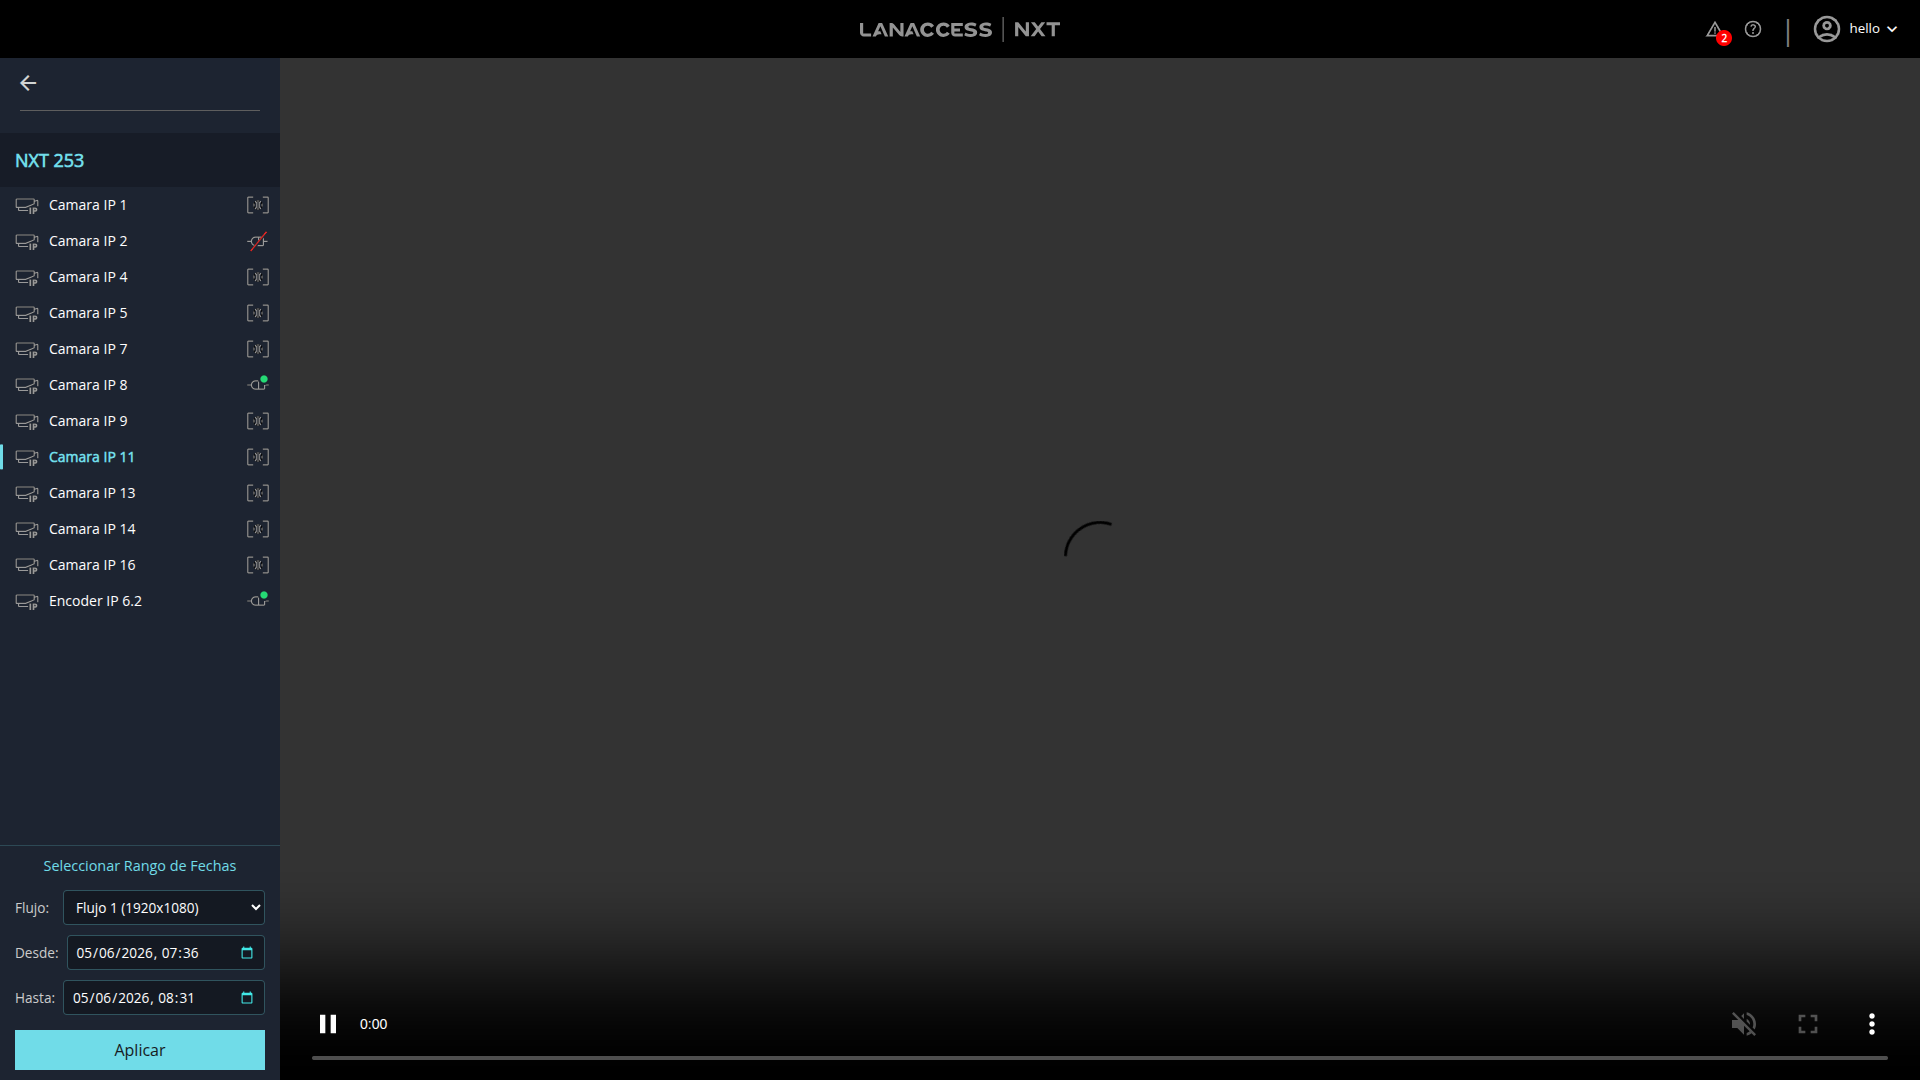
\includegraphics[width=0.95\textwidth]{figures/ui_recordings.png}
  \caption{Vista del reproductor de vídeo històric i component interactiu Timeline.}
  \label{fig:ui_recordings}
\end{figure}

\subsection{El Servidor de Segmentació de Vídeo (la-video-engine Backend)}
El motor de gravacions s'ha dissenyat sota un enfocament de transmissió eficient basat en el protocol estàndard \textbf{HLS} (\textit{HTTP Live Streaming}). El repte tècnic principal del costat del servidor residia en la impossibilitat d'enviar fitxers sencers d'enregistrament degut a l'enorme consum d'ample de banda i memòria RAM que requeriria.

Per resoldre-ho, el microservei \textbf{la-video-engine} (desenvolupat en C++) implementa un pipeline de segmentació multimèdia en temps real que actua sota demanda:
\begin{enumerate}
  \item \textbf{Indexació i Cerca:} Quan el client demana una franja de temps, el servidor interroga directament la base de dades local de l'NVR per localitzar els fitxers d'enregistrament físics afectats.
  \item \textbf{Segmentació Dinàmica (Trans-muxing):} El servidor llegeix els descriptors d'arxiu i, sense realitzar una transcodificació completa (el que sobrecarregaria de manera inacceptable la CPU del gravador), extreu els paquets de vídeo i els empaqueta o encapsula de forma asíncrona en contenidors de transport elementals estàndard MPEG-TS (fitxers \texttt{.ts}) de pocs segons de durada.
  \item \textbf{Generació de Playlist:} El servidor genera un fitxer d'índex o llista de reproducció XML/m3u8 dinàmica (fitxer \texttt{.m3u8}) que apunta a aquests segments temporals virtuals sota un identificador únic o token de sessió temporal de reproducció.
\end{enumerate}

\subsection{El Client de Playback i la Línia de Temps Interactiva (Timeline)}
A l'interfície web (Figura \ref{fig:ui_recordings}), el disseny es divideix en un calendari d'elecció de data, un seccionador de càmeres i una línia de temps interactiva de dades de tipus \textit{Timeline} situada a la part inferior. El cicle de funcionament del frontend segueix els passos següents:

\begin{enumerate}
  \item El client demana l'índex de gravacions per a un dia seleccionat mitjançant el component \texttt{DateTimeRangeSelectorComponent}.
  \item El frontend rep un llistat de metadades amb les franges temporals exactes en què s'ha emmagatzemat vídeo.
  \item El motor de renderitzat dibuixa gràficament la línia de temps utilitzant un codi de colors altament intuïtiu per a l'operador: verd/blau per a gravació de tipus continu, i vermell/taronja per a gravació disparada per un esdeveniment d'alarma o analítica.
  \item En fer clic o desplaçar el lliscador del timeline, el frontend calcula el *timestamp* exacte de destí i demana al segmentador de l'NVR la llista de reproducció específica a través de la crida d'escriptura \texttt{loadVideo()} (vegeu el llistat \ref{lst:hls_load_code}).
\end{enumerate}

\begin{lstlisting}[language=JavaScript, label={lst:hls_load_code}, caption={Càrrega dinàmica de llista de reproducció HLS basada en franges de temps.}]
loadVideo(): void {
  const token = this.selectedToken();
  if (this.hls) {
    this.hls.destroy();
    this.hls = undefined;
  }
  if (!this.videoPlayer || !this.selectedCamera() || !token) return;

  const videoElement = this.videoPlayer.nativeElement;
  const start = Math.floor(this.recordingStartTime().getTime() / 1000);
  const end = Math.floor(this.recordingEndTime().getTime() / 1000);
  
  // Construccio de la URL del segmentador dinamic del la-video-engine
  const hlsUrl = `/video-engine/hls-play.m3u8?token=${token}&start=${start}&end=${end}`;

  if (Hls.isSupported()) {
    this.hls = new Hls({
      maxBufferHole: 4.0,          // Tolerancia a buits de dades
      manifestLoadingTimeOut: 20000 // Temps d'espera de xarxa per al manifest
    });
    this.hls.loadSource(hlsUrl);
    this.hls.attachMedia(videoElement);
    this.hls.on(Hls.Events.MANIFEST_PARSED, () => {
      videoElement.play().catch(err => console.warn('Play prevented', err));
    });
  }
}
\end{lstlisting}

\subsection{Coexistència i Descodificació de Còdecs H.264 i H.265}
Un dels reptes de disseny més rellevants abordat en la programació unificada del frontend i el backend és la compatibilitat asíncrona amb els còdecs d'última generació **H.265 (HEVC)** de manera transparent al costat d'**H.264 (AVC)**.

Tot i que el format H.265 permet reduir a la meitat l'espai necessari als discs durs de gravació de l'NVR per a la mateixa qualitat d'imatge (la qual cosa representa un valor comercial i operatiu enorme), el seu suport de descodificació nativa dins dels navegadors web ha estat històricament molt restringit per qüestions de patents, forçant tradicionalment l'empresa a dependre d'aplicacions locals pesades o controls ActiveX.

Amb el nou disseny, el motor de segmentació \textbf{la-video-engine} preserva el còdec d'origen de l'enregistrament de la càmera durant l'empaquetat del segment TS. Durant l'execució al navegador:
\begin{itemize}
  \item El client web d'Angular detecta de forma transparent les capacitats de descodificació per maquinari de la targeta gràfica (GPU) del dispositiu de l'operador.
  \item Si el dispositiu és modern i el navegador web suporta descodificació HEVC, l'NVR transmet els fragments H.265 directament per maximitzar l'estalvi d'ample de banda.
  \item En cas contrari, o si la càmera utilitzada és antiga, el sistema commuta de manera unificada cap a H.264, oferint una fluïdesa total en qualsevol tipus de terminal i garantint una interfície lliure d'instal·lació de complements externs (*Plugin-free*).
\end{itemize}

\section{Sistema d'Alarmes i Comunicació Asíncrona Multi-capa}
La gestió, notificació i persistència d'esdeveniments d'alarma en temps real constitueix un dels requisits no funcionals més crítics del dispositiu, atès que qualsevol retard o pèrdua de dades compromet la seguretat de la instal·lació. En el marc d'aquest projecte, s'ha dissenyat i desenvolupat íntegrament una solució de comunicació multi-capa extrem a extrem: des del model de subscripció reactiva al \textit{frontend} d'Angular 19, passant per les passarel·les de WebSockets d'alta velocitat, fins a arribar al sistema de persistència transaccional de baix nivell al sistema operatiu embedded de l'NVR.

Per tal de conceptualitzar aquest flux d'informació complex, a continuació es descriu la topologia del canal de persistència i propagació d'alarmes des del maquinari fins a la base de dades i l'interfície gràfica d'usuari (UI):

\begin{center}
  \small
  \texttt{[Maquinari/Càmeres]} $\rightarrow$ \texttt{[D-Bus]} $\rightarrow$ \texttt{[la-core-alarm]} $\xrightarrow{\text{gRPC}}$ \texttt{[la-db-engine (VFS Driver)]} \\
  $\xrightarrow{\text{Unix Socket}}$ \texttt{[la-video-engine]} $\xrightarrow{\text{Escriptura}}$ \texttt{[Disc Físic (SQLite3)]} \\
  $\xleftarrow{\text{Lectura/WSS}}$ \texttt{[la-core-notifier / NGINX]} $\xleftarrow{\text{Observable Shared}}$ \texttt{[Frontend Angular 19]}
\end{center}

\subsection{Disseny de Persistència: El Virtual File System (VFS) i Unix Sockets}
Per garantir la transaccionalitat i robustesa de les alarmes (propietats ACID) davant de talls d'energia sobtats, s'ha utilitzat el motor de bases de dades relacional \textbf{SQLite3}. No obstant això, per complir amb les directives de seguretat de sistemes crítics i evitar conflictes de concurrència d'accés a disc (fitxers blocats), s'ha implementat un mètode de persistència altament desacoblat:

\begin{enumerate}
  \item \textbf{El servei d'orquestració (\texttt{la-db-engine}):} Aquest microservei actua com a gestor de la base de dades de dades, de la lògica de consultes SQL i de la comunicació cap al servei d'alarmes mitjançant crides binàries d'alt rendiment \textbf{gRPC}. Tanmateix, per política de seguretat, aquest procés està aïllat en un espai d'usuari (\textit{sandbox}) i no té permisos d'escriptura directa sobre el disc dur.
  \item \textbf{El Driver de VFS Personalitzat:} Per resoldre aquesta restricció, es va dissenyar i registrar un driver de fitxers virtuals personalitzat o **Virtual File System (VFS)** de SQLite3 dins del codi de \texttt{la-db-engine}. Aquest driver intercepta qualsevol crida del motor de la base de dades que requereixi realitzar una escriptura física a disc (com un *commit* de transacció de nova alarma).
  \item \textbf{La Passarel·la per Unix Sockets:} En lloc d'intentar obrir el fitxer de base de dades local, el driver VFS serialitza el bloc d'operacions d'E/S i el transmet immediatament a través d'un canal de comunicació entre processos (IPC) de tipus **Unix Domain Socket** cap al servei \textbf{la-video-engine} (l'únic dimoni del sistema autoritzat a interactuar directament amb la controladora de disc d'emmagatzematge). El motor de vídeo rep els canvis, aplica les regles i realitza l'escriptura persistent de manera absolutament transparent per al motor de base de dades.
\end{enumerate}

\subsection{Optimització del Frontend i Consum de Sockets}
Per al control dels esdeveniments en temps real des de la interfície de client, s'ha implementat un canal de \textbf{WebSockets Segurs (WSS)} unificat mitjançant el patró de disseny **Observer**.

A nivell de client, l'obertura de túnels de comunicació és una operació costosa per a la CPU del gravador embedded i per al servidor d'NGINX. Per evitar que cada component d'interfície o element del DOM que demani dades en temps real (com el mosaic de vídeo, la taula d'alarmes o l'indicador de la capçalera) obri una connexió independent cap a \texttt{la-core-notifier}, s'ha programat un **servei de missatgeria unificat** sota el patró \textit{Observable Shared} (vegeu la Figura \ref{fig:ui_alarms}).

\begin{figure}[htbp]
  \centering
  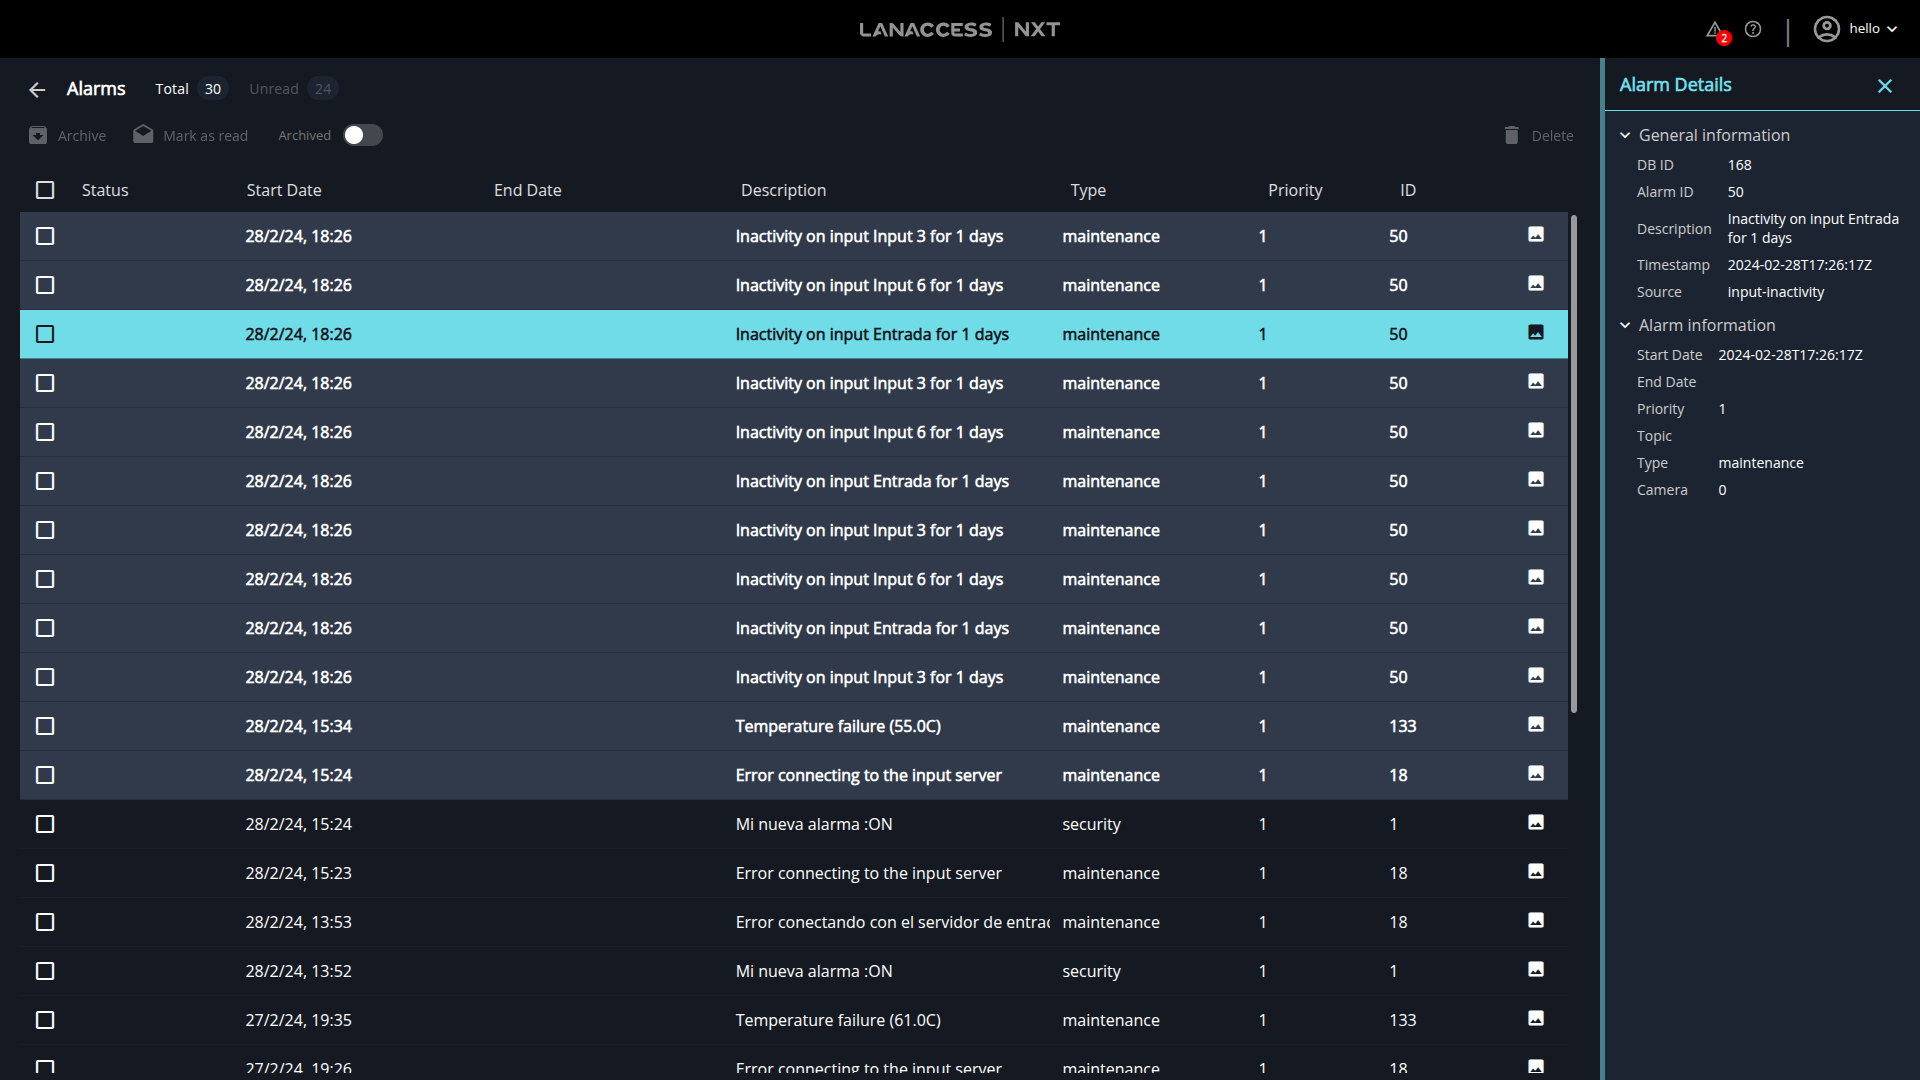
\includegraphics[width=0.95\textwidth]{figures/ui_alarms.png}
  \caption{Taula de monitoratge d'alarmes en temps real i botons d'assentiment.}
  \label{fig:ui_alarms}
\end{figure}

Mitjançant la utilització del pipeline d'RxJS i l'operador \texttt{shareReplay({bufferSize: 1, refCount: true})}, els diferents components de l'aplicació s'acoblen com a subscriptors actius d'una única connexió compartida. L'obertura de sockets es redueix exactament a un canal, el qual es tanca de manera automàtica quan l'usuari surt de les seccions asíncrones de l'aplicació, optimitzant el rendiment global de la memòria de l'equip de xarxa.

\subsection{El Cicle de Vida de l'Alarma i la Robustesa davant de Talls}
Quan el client d'Angular rep un missatge d'esdeveniment a través del canal, l'estat global s'actualitza immediatament, fent que la taula d'alarmes es redibuixi de manera reactiva mitjançant l'ús de \textbf{Signals}. Les alarmes passen per un cicle d'estats descrit a la Figura \ref{fig:state_alarm}:

\begin{figure}[!htbp]
  \centering
  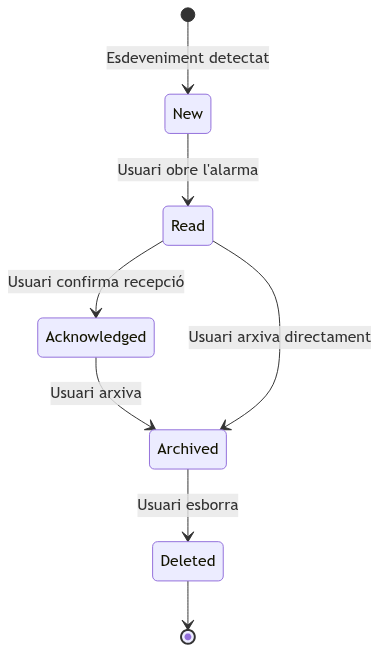
\includegraphics[width=0.55\textwidth]{figures/state_alarm.png}
  \caption{Diagrama d'estats del cicle de vida de les alarmes.}
  \label{fig:state_alarm}
\end{figure}

L'operador pot interaccionar amb cadascun dels incidents per tal d'assentir-los (\textit{Acknowledgment}) fent clic sobre el botó \textit{Ack} al final de la fila. Aquesta operació tanca l'estat actiu de la incidència lògica a l'NVR i silencia el led vermell físic de la placa del videogravador.

Per garantir la continuïtat del servei d'alertes en entorns de xarxa inestables o davant d'interrupcions temporals de la connectivitat del client, la connexió s'ha programat amb una lògica de **reconnexió i Backoff Exponencial** asíncrona:

\begin{lstlisting}[language=JavaScript, caption={Connexió WebSocket resilient amb backoff exponencial en RxJS.}]
this.socket$.pipe(
  retry({
    delay: (error, retryCount) => {
      // 1. Si l'usuari perd la seva sessio, avorta els intents de reconexio
      if (!this.userService.isAuthenticated()) {
        return throwError(() => new Error('Connexio tancada per perdua de credencials.'));
      }
      
      // 2. Incrementa de manera exponencial el temps d'espera per evitar DoS al NVR
      const nextDelay = RECONNECT_INTERVAL_MS * retryCount;
      console.warn(`[WS] Connexio perduda. Intentant reconexio #${retryCount} en ${nextDelay}ms.`);
      return timer(nextDelay); 
    },
  })
).subscribe({
  next: (message) => this.messagesSubject$.next(message)
});
\end{lstlisting}

Aquest disseny asíncron evita que, davant d'un tall generalitzat de xarxa, centenars de clients inundin simultàniament la CPU del videogravador embedded amb peticions agresives de reconnexió, espaiant de manera intel·ligent les cerques fins a restaurar l'estat segur amb el component unificat d'error de connexió.

\subsection{Estructures de Missatges del Canal Asíncron (WebSockets)}
Per documentar el rigor de la integració, a continuació es detallen els missatges JSON que viatgen a través d'aquest servei de notificacions unificat.

El primer missatge que s'envia (Client $\rightarrow$ Servidor) serveix per inicialitzar i subscriure's només a la telemetria desitjada, estalviant amplada de banda:
\begin{lstlisting}[language=json, caption={Missatge d'inicialització del filtre de subscripció.}]
{
  "type": "filter_update",
  "transactionId": "home-page-filter-2026-03-30/12:00:00.123",
  "payload": {
    "include_topics": ["device/notification", "io"]
  }
}
\end{lstlisting}

Quan una entrada digital canvia el seu estat físic, el servidor envia automàticament la notificació següent (Servidor $\rightarrow$ Client):
\begin{lstlisting}[language=json, caption={Notificació asíncrona de canvi d'estat d'E/S.}]
{
  "event": "IO_NOTIFY",
  "payload": [
    {
      "id": "01",
      "idr": "01",
      "data": "on",
      "time": "2026-03-30T12:01:15Z",
      "topic": "io/input"
    }
  ]
}
\end{lstlisting}

Finalment, en el cas de rebre una alarma crítica des de la base de dades (com una intrusió generada des de \textbf{la-core-alarm}), el format inclou totes les metadades persistides a SQLite3:
\begin{lstlisting}[language=json, caption={Notificació d'alarma en temps real de la base de dades.}]
{
  "event": "DB_ENGINE_ALARM_NOTIFY",
  "payload": [
    {
      "alarm_id": "AL_05",
      "db_id": "1054",
      "description": "Intrusio Zona Nord",
      "priority": "1",
      "source": "Camera 3",
      "start_date": "2026-03-30T12:05:00Z",
      "end_date": "-",
      "status": "active",
      "timestamp": "1711800300",
      "topic": "db/alarms",
      "type": "security",
      "camera_num": "3",
      "is_read": false,
      "is_archived": false,
      "is_locked": false
    }
  ]
}
\end{lstlisting}

\section{Manteniment i Gestió de la Infraestructura del Maquinari}
El darrer bloc operatiu d'aplicació d'enginyeria de la plataforma engloba les funcionalitats administratives de suport, dissenyades per allargar la vida útil, facilitar el diagnòstic remot, garantir la traçabilitat de les accions i mantenir la integritat lògica del videogravador. Aquest conjunt d'eines s'ha programat íntegrament en el client d'Angular 19 i es comunica directament amb les APIs d'administració de \textbf{la-core-legacy} i \textbf{la-video-engine}.

\subsection{Mòdul d'Actualització Remota del Firmware}
L'actualització de firmware és un procés crític en sistemes embedded de seguretat, ja que una fallida d'alimentació o d'escriptura durant el procés d'escriptura (\textit{flashing}) pot deixar el dispositiu inutilitzable. Per minimitzar aquest risc i proporcionar una monitorització en temps real a l'operador, s'ha dissenyat un sistema d'actualització robust i tolerant a fallides estructurat en tres fases d'execució:

\begin{figure}[htbp]
  \centering
  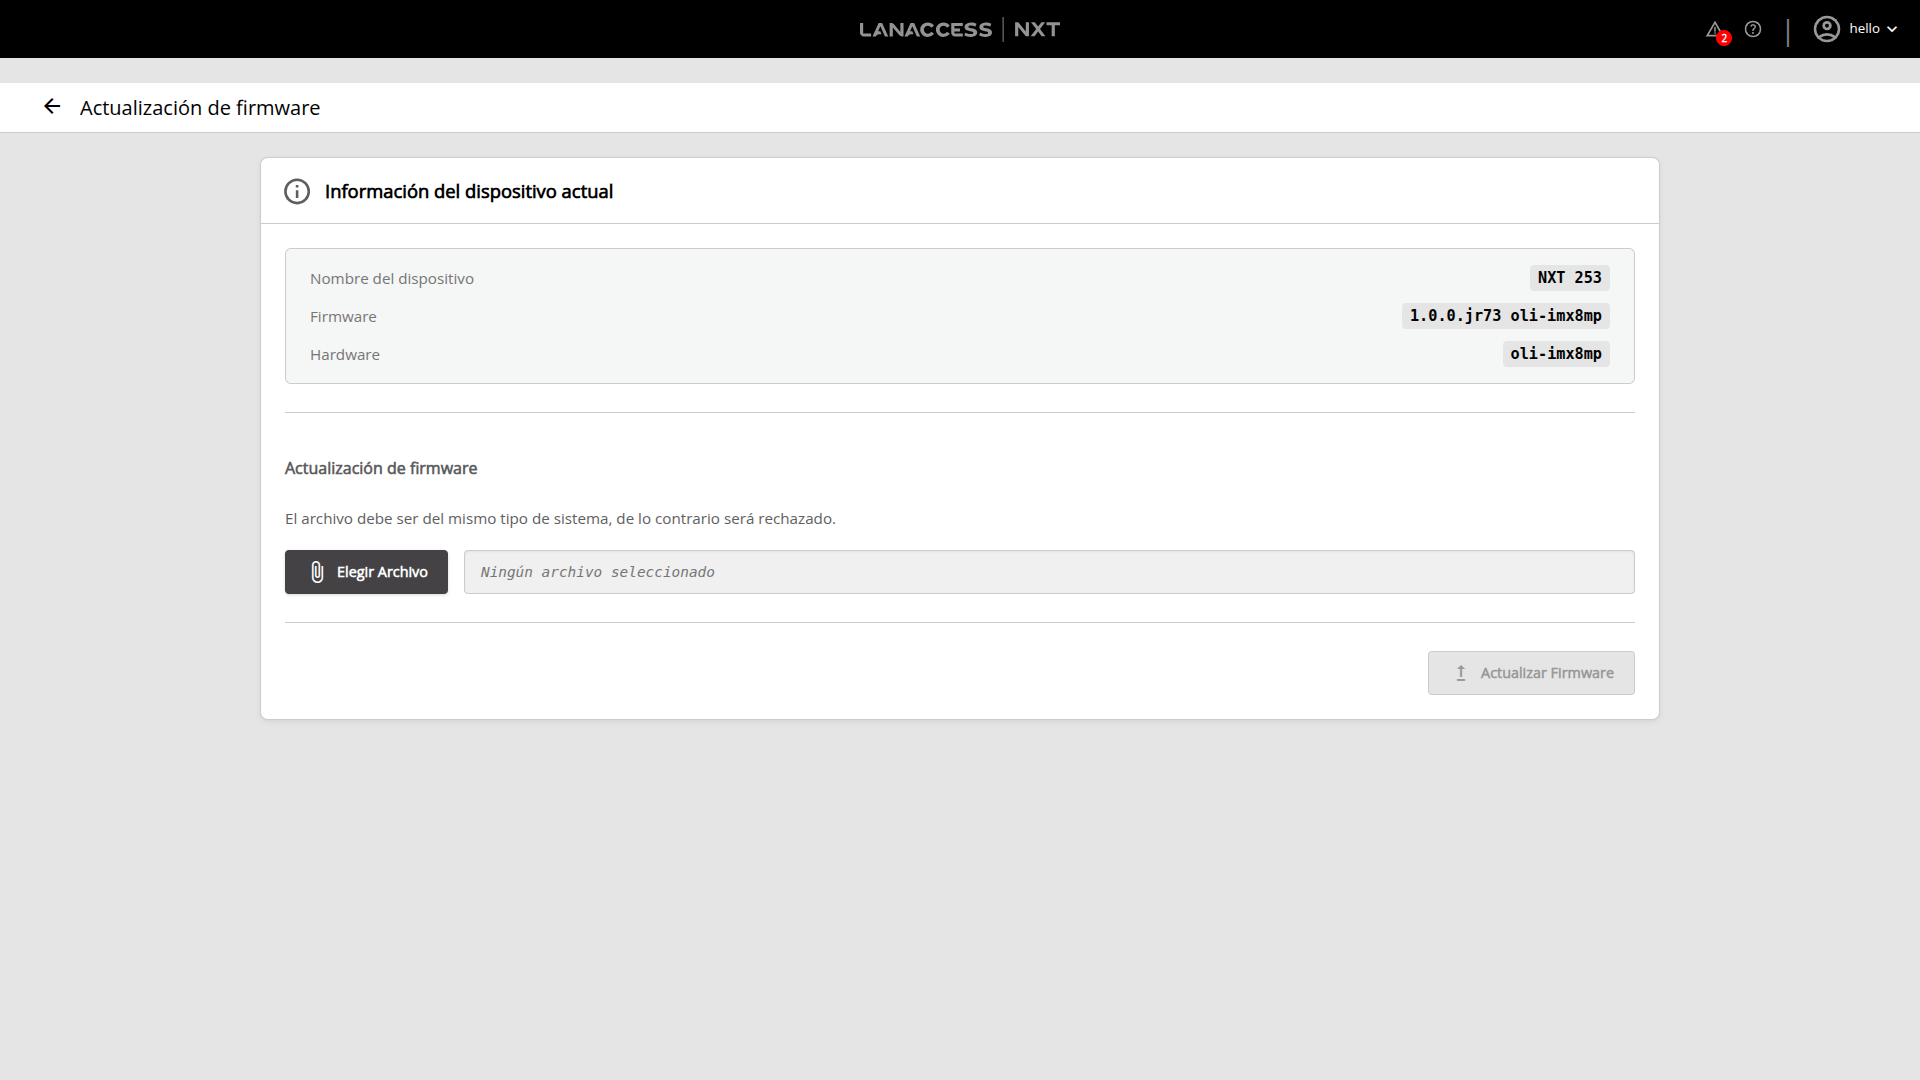
\includegraphics[width=0.95\textwidth]{figures/ui_update.png}
  \caption{Mòdul d'actualització per seleccionar arxius de firmware.}
  \label{fig:ui_update}
\end{figure}

\begin{enumerate}
  \item \textbf{Càrrega i Validació (Figura \ref{fig:ui_update}):} L'operador selecciona el fitxer binari d'actualització (\texttt{.bin}). El frontend valida en primer lloc la firma, l'extensió i la mida del fitxer al navegador abans d'iniciar una petició POST d'escriptura multipart cap a l'endpoint de \texttt{la-core-legacy}.
  \item \textbf{Sondeig d'Estat (\textit{Polling} de Flashing):} Un cop completada la pujada del fitxer, l'aplicació web inicia un procés de consulta periòdica de l'estat cap a \texttt{/webprotocol/firmware\_upgrade\_state} (vegeu la Figura \ref{fig:ui_updating_prog}). L'aplicació mapeja l'estat rebut a la barra de progrés reactiva:
        \begin{itemize}
          \item \texttt{UPLOADING / WAITING:} El fitxer s'està transferint i validant internament.
          \item \texttt{UPDATING:} El sistema està escrivint el nou binari a la partició de firmware secundària des de la memòria d'emmagatzematge temporal.
          \item \texttt{REBOOTING:} S'ordena el reinici del sistema físic.
          \item \texttt{ERROR / INCONSISTENT:} El procés es cancel·la a causa de dades corrompudes o errors de xarxa, activant immediatament la lògica de retorn segur a la partició anterior (\textit{dual-boot rollback}).
        \end{itemize}
  \item \textbf{Recuperació de la Connectivitat (Figura \ref{fig:ui_updating_reboot}):} Quan s'inicia el reinici físic del gravador, l'aplicació web bloqueja la interfície amb una pantalla d'espera i s'absté de fer peticions durant 15 segons de marge segur. Transcorregut aquest temps, inicia un procés de consulta ràpida de la connectivitat IP de xarxa (\texttt{connectivity.cgi}). Un cop restablerta la connexió, es verifica l'èxit definitiu de l'operació preguntant l'estat lògic final, i es permet l'accés un altre cop a la interfície.
\end{enumerate}

\begin{figure}[htbp]
  \centering
  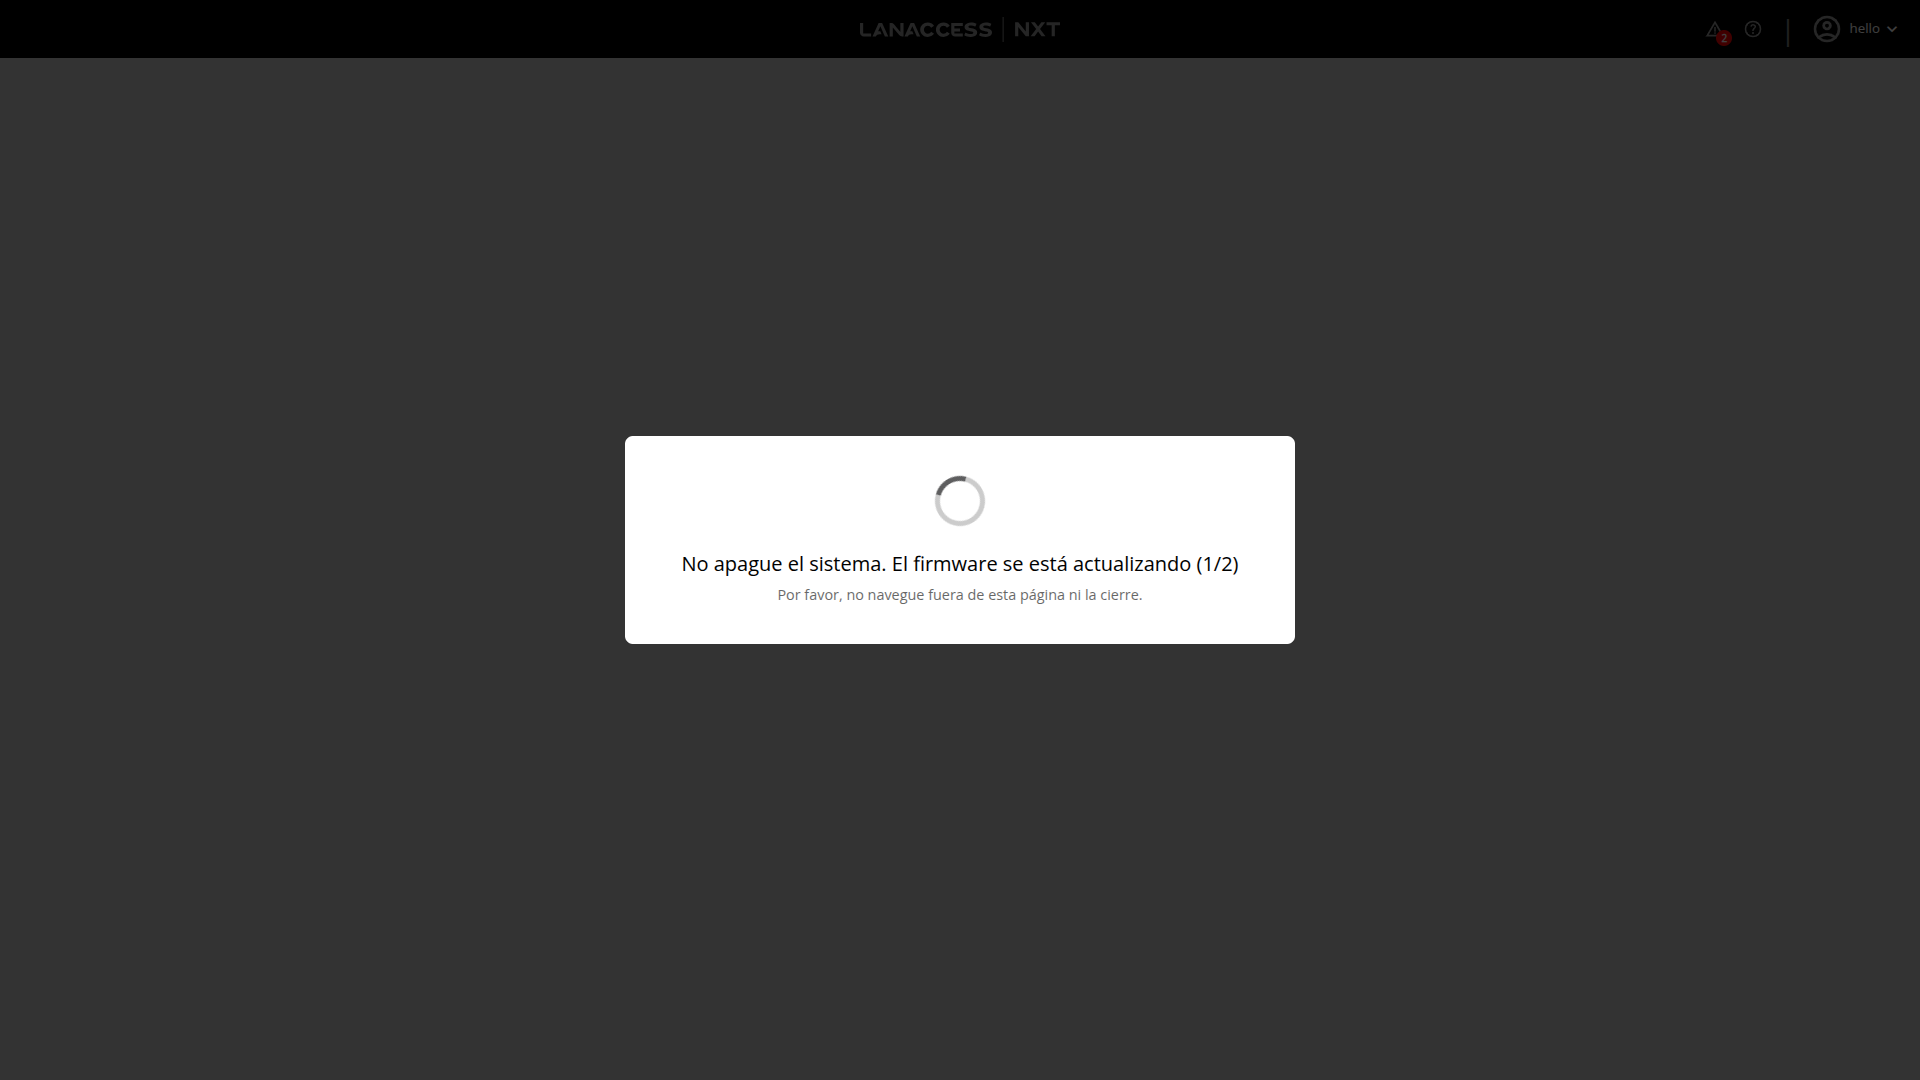
\includegraphics[width=0.48\textwidth]{figures/ui_updating1.png}
  \hfill
  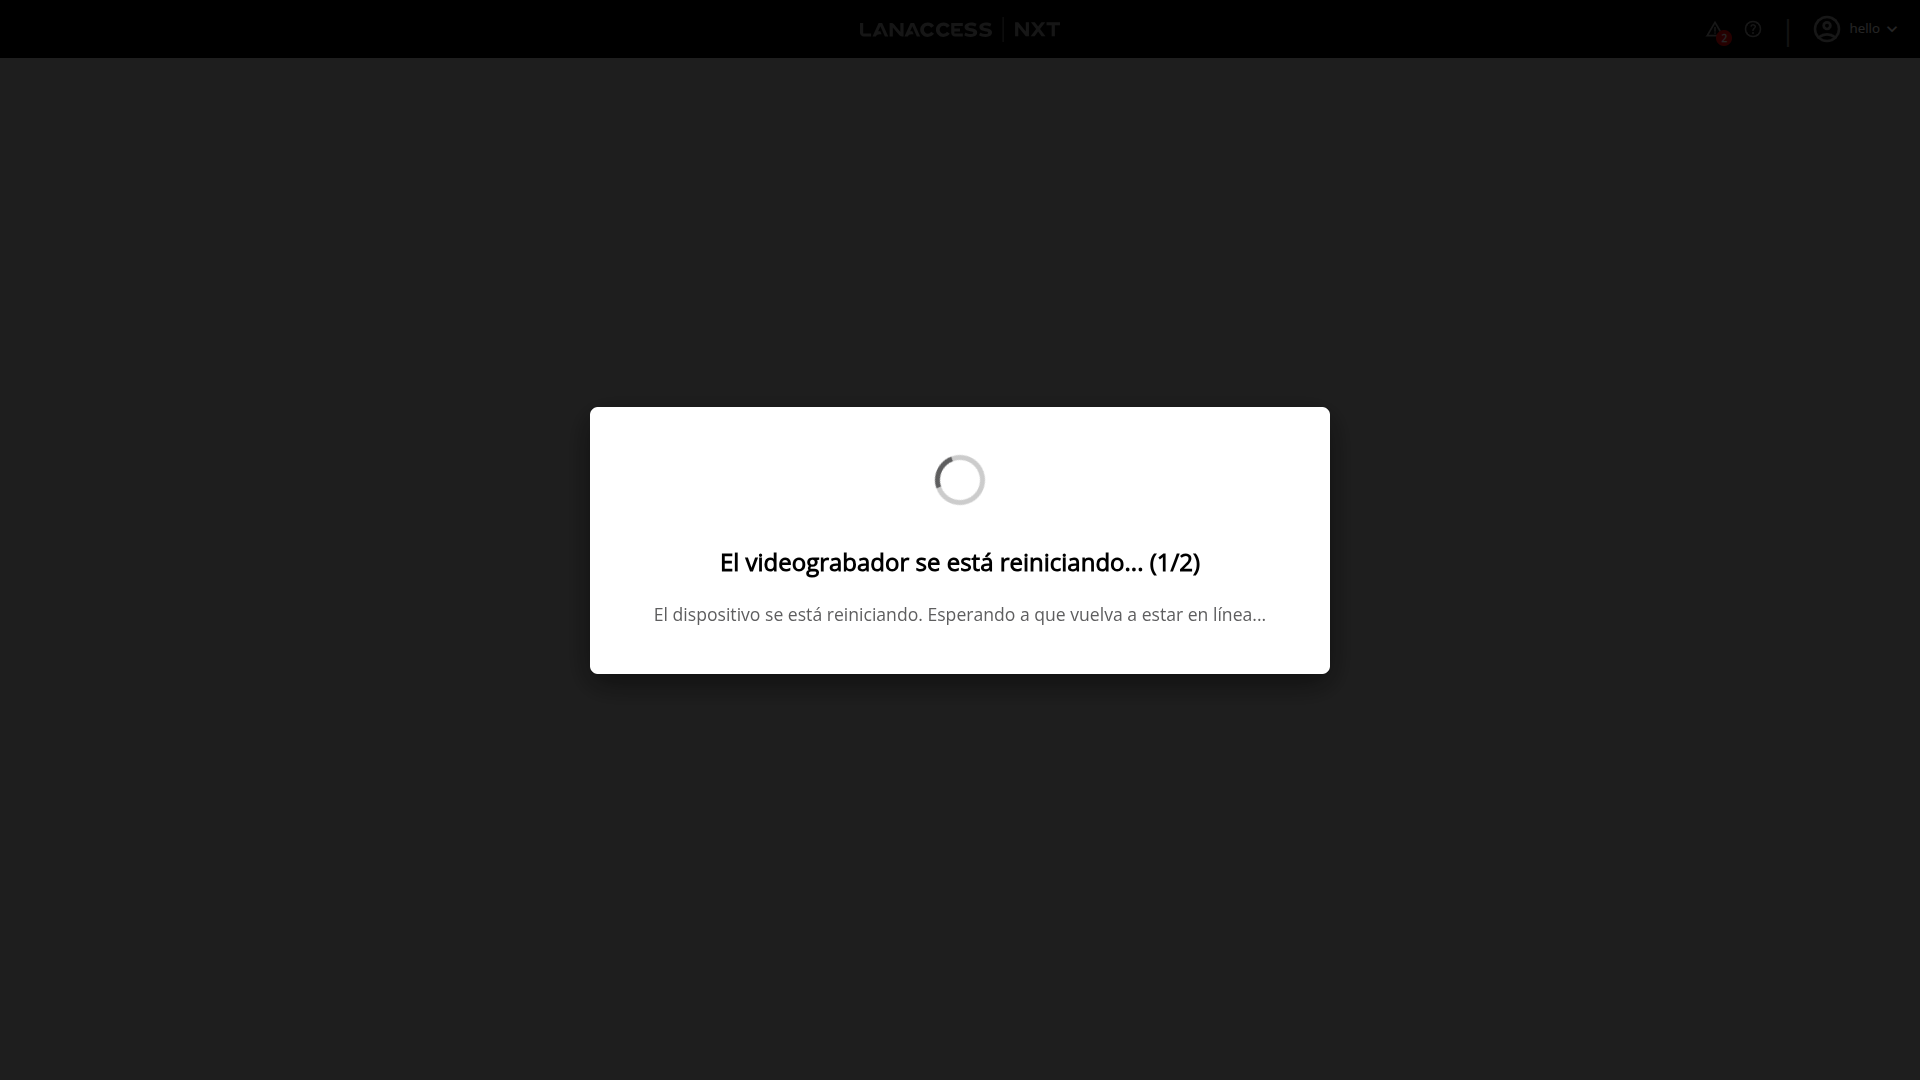
\includegraphics[width=0.48\textwidth]{figures/ui_updating2.png}
  \caption{Barra de progrés reactiva i fases d'escriptura (\textit{flashing}).}
  \label{fig:ui_updating_prog}
\end{figure}

\begin{figure}[htbp]
  \centering
  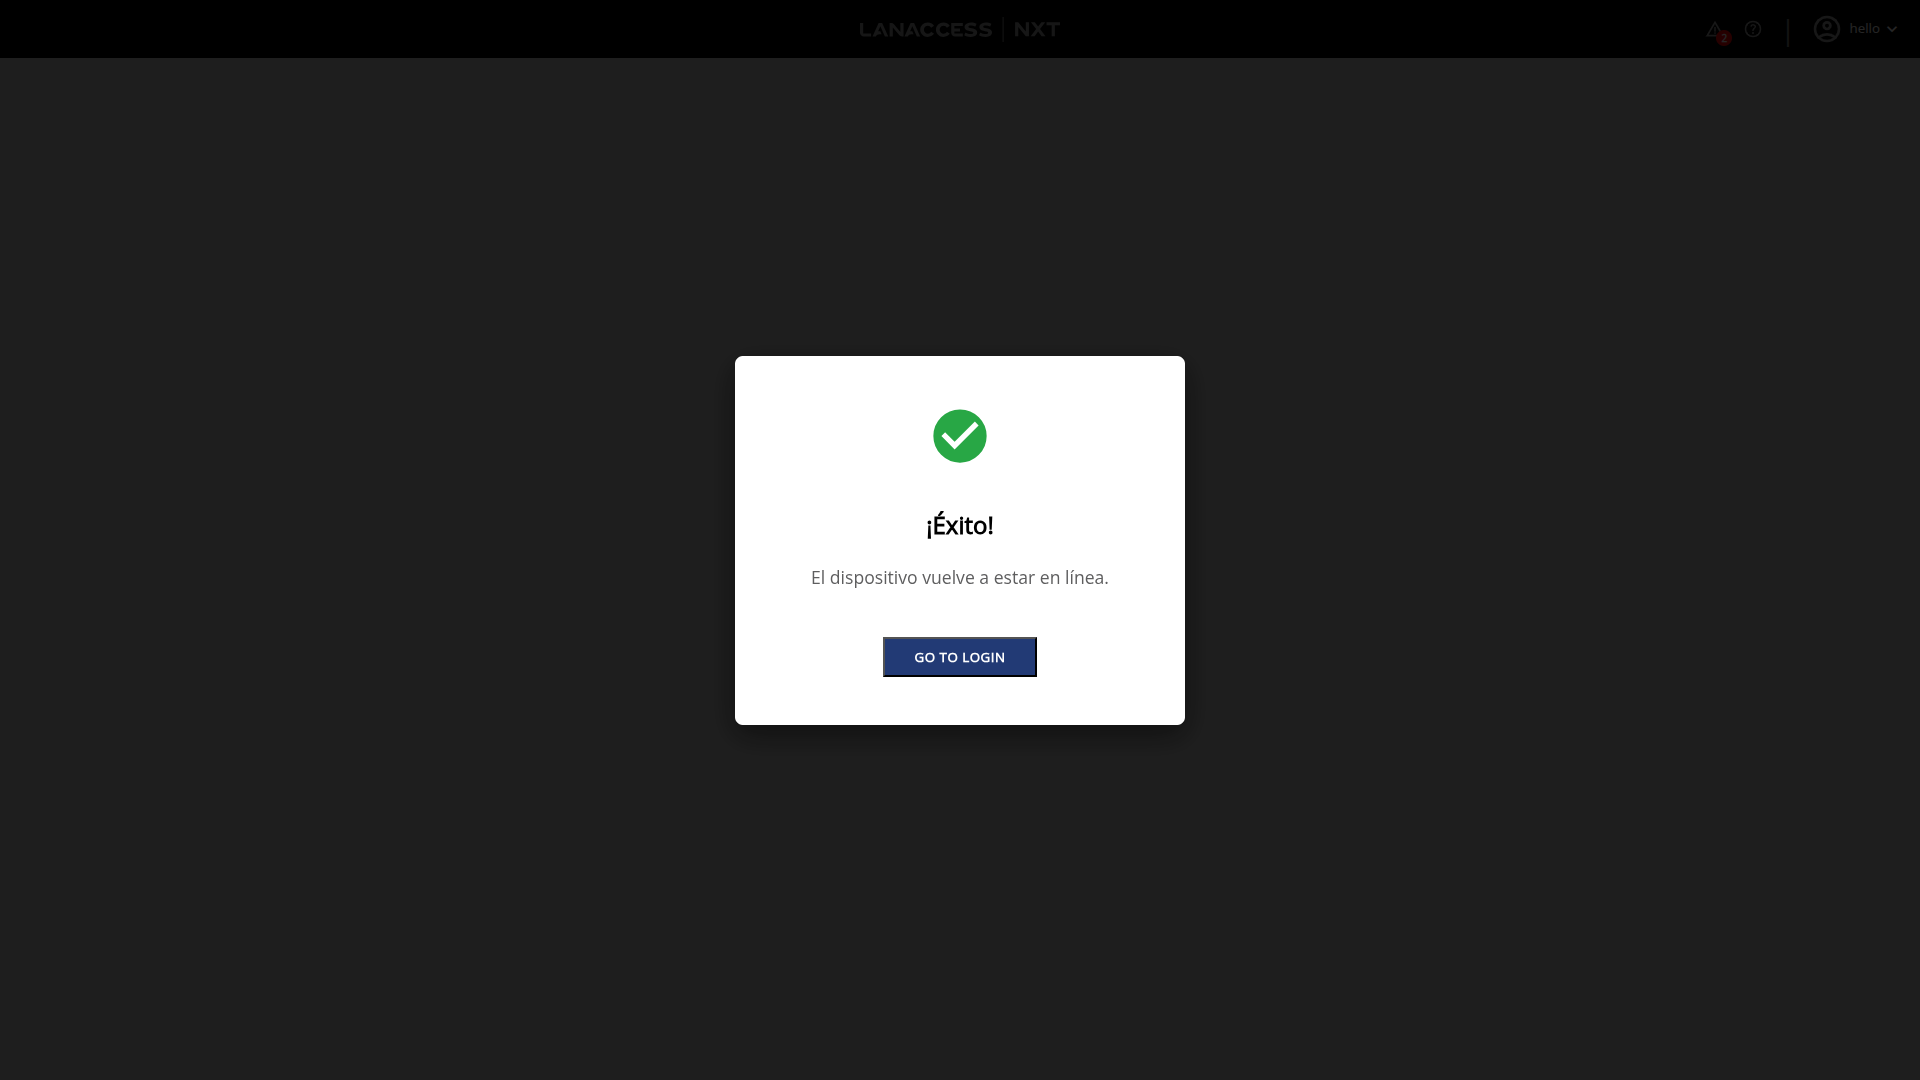
\includegraphics[width=0.95\textwidth]{figures/ui_updating3.png}
  \caption{Pantalla de reinici automàtic amb poldeig de reconnectivitat.}
  \label{fig:ui_updating_reboot}
\end{figure}

\subsection{Mòdul d'Accions Globals: Còpies de Seguretat i Restauració de Fàbrica}
El panell d'accions de configuració unifica les comandes administratives destructives i de salvaguarda de dades (Figura \ref{fig:ui_configuration_actions}).

\begin{figure}[htbp]
  \centering
  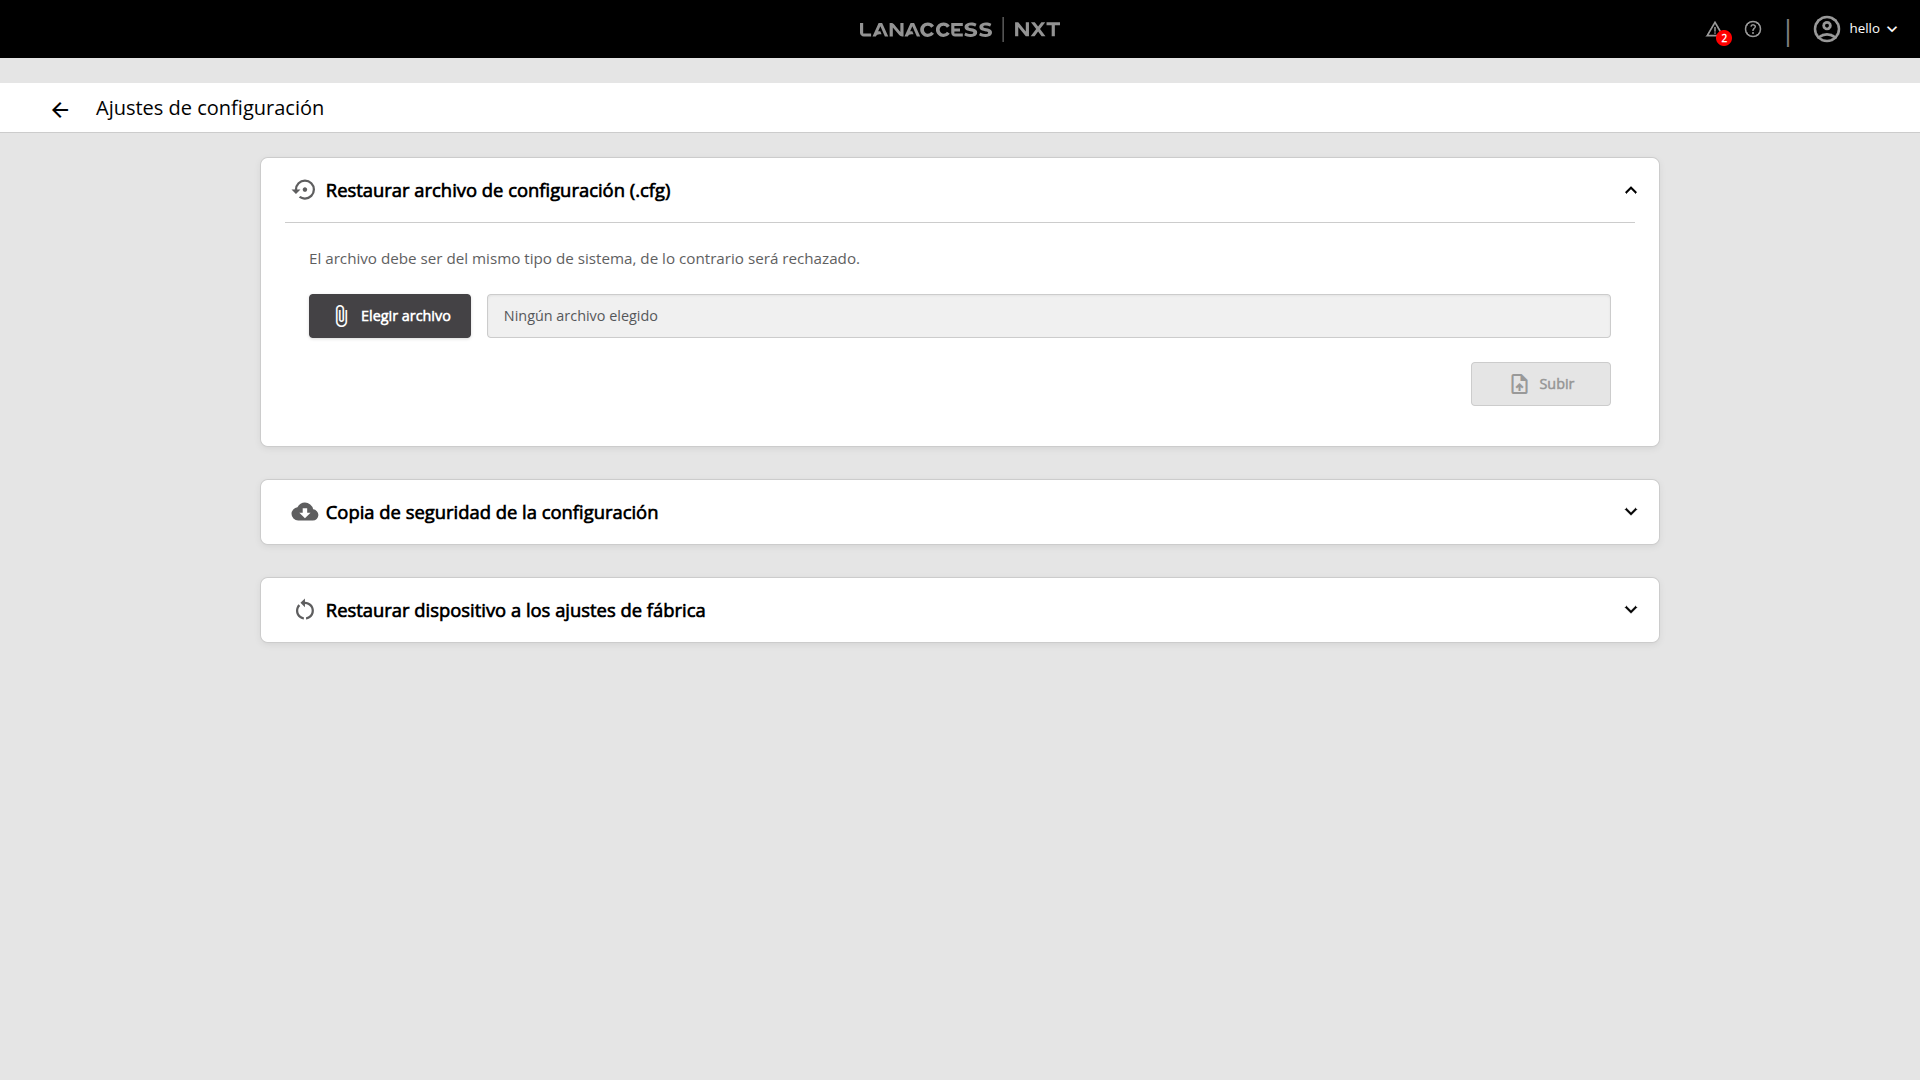
\includegraphics[width=0.95\textwidth]{figures/ui_configuration.png}
  \caption{Accions globals de manteniment: Backup, Restore i Reset de Fàbrica.}
  \label{fig:ui_configuration_actions}
\end{figure}

\begin{itemize}
  \item \textbf{Còpia de Seguretat (Backup):} El frontend sol·licita l'exportació de la base de dades. El servidor munta un fitxer binari unificat amb extensió \texttt{.cfg}. Per motius de seguretat, les contrasenyes i dades de tipus \texttt{password} s'exclouen d'aquesta llista i es substitueixen per la clau enmascarada \texttt{\_\_reserved\_pwd\_} per evitar l'exposició d'identitats de connexió.
  \item \textbf{Restauració de Còpia (Restore):} Permet pujar un fitxer de configuració del tipus \texttt{.cfg} compatible. S'incorpora l'opció \texttt{preserveNetwork} dissenyada per evitar que l'instal·lador o tècnic de camp perdi la connexió de xarxa en entorns de xarxa remots en cas que s'hagi de carregar una configuració heretada amb un enrutament diferent.
  \item \textbf{Restabliment de Fàbrica (Factory Reset):} Permet retornar la base de dades a l'estat d'origen. Per evitar la pèrdua accidental de dades o atacs de tipus CSRF, s'imposa un mètode securitzat en dues fases: el client demana primer un token d'autorització d'escriptura de canvis d'un sol ús (\textit{Token de seguretat}) a la-core-legacy, i només si és vàlid, es pot processar la crida destructiva.
\end{itemize}

\subsection{Visor d'Auditoria i Registre de Successos (Logs)}
El visor de registres (Figura \ref{fig:ui_log}) s'ha programat per complir de manera rigorosa amb la normativa de seguretat **UNE-EN 62676**, que exigeix la traçabilitat absoluta i inalterable d'accions sensibles (com ara qui ha visualitzat quin canal de vídeo històric, en quines dates i hores exactes, o quins intents fallits d'accés s'han produït).

\begin{figure}[htbp]
  \centering
  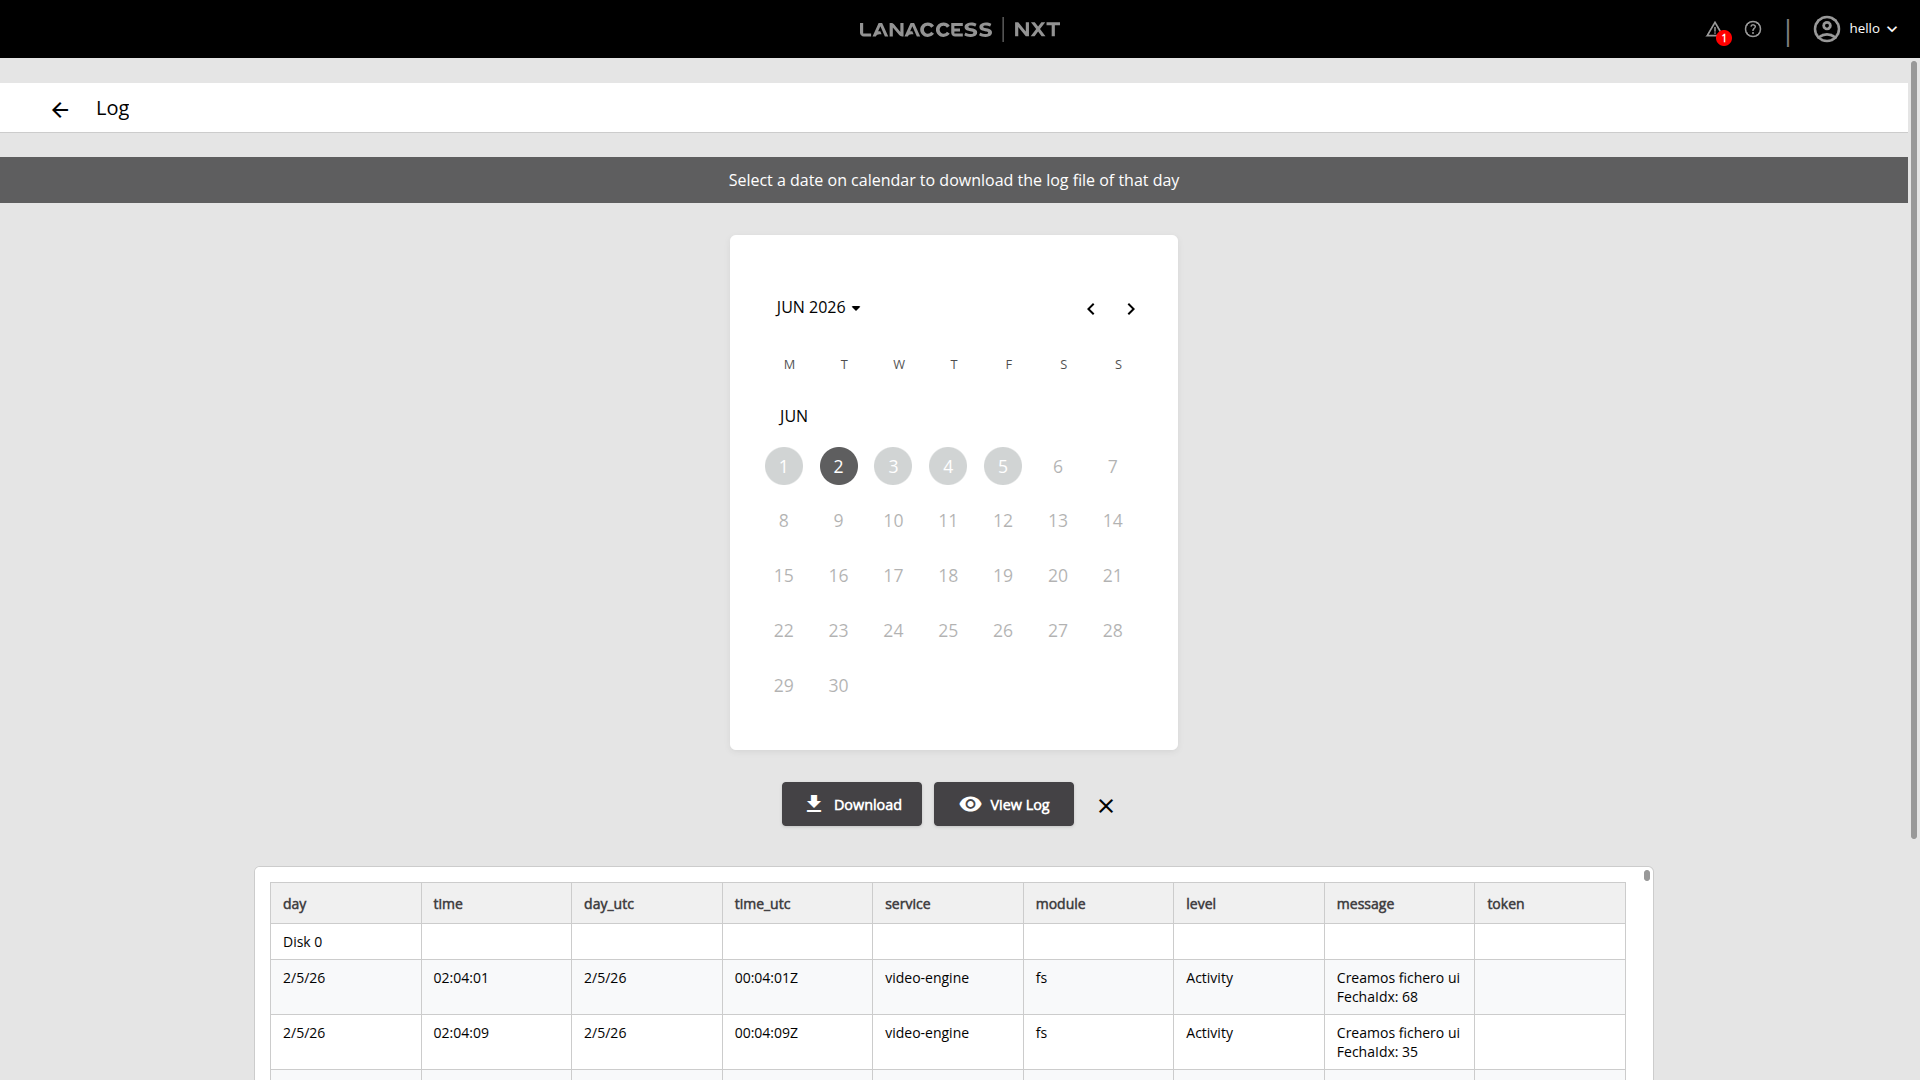
\includegraphics[width=0.95\textwidth]{figures/ui_log.png}
  \caption{Visor de registres i auditories amb filtres temporals i descàrrega.}
  \label{fig:ui_log}
\end{figure}

Per poder treballar amb volums de dades molt grans que poden superar les 500.000 files de successos per setmana, s'ha dissenyat un mètode de visualització optimitzat en dues capes que evita el col·lapse de la memòria RAM del navegador de l'usuari:
\begin{enumerate}
  \item \textbf{Sondeig de Calendari:} Abans de pintar la interfície del calendari, l'aplicació consulta a través de \texttt{commonCalendarGetDays.cgi} quins dies tenen fitxers de registre disponibles. El frontend marca exclusivament els dies actius al selector, evitant que l'operador hagi d'interrogar dates buides.
  \item \textbf{Processat de Dades amb SheetJS:} Quan es selecciona un dia vàlid, es demana l'historial a \texttt{listlog.cgi} com un fitxer binari xifrat estructurat. En lloc de renderitzar directament milers de línies al DOM (el que provocaria el bloqueig de la interfície de l'usuari), el frontend utilitza la llibreria \texttt{XLSX} (SheetJS) per parsejar les dades a nivell de memòria d'execució. El sistema organitza les dades en una taula reactiva de descàrrega i filtre local per paraula clau, permetent una navegació extremadament fluida.
\end{enumerate}

\subsection{Mòdul d'Ajuda i Documentació Integrada (Air-Gapped Operation)}
En entorns industrials o de màxima seguretat, és habitual que els gravadors NVR treballin en una xarxa aïllada físicament del món exterior (funcionament en entorns \textit{air-gapped}). En aquests casos, quan un tècnic necessita consultar una guia d'instruccions, no pot accedir a internet ni connectar-se a servidors corporatius de suport externs.

\begin{figure}[htbp]
  \centering
  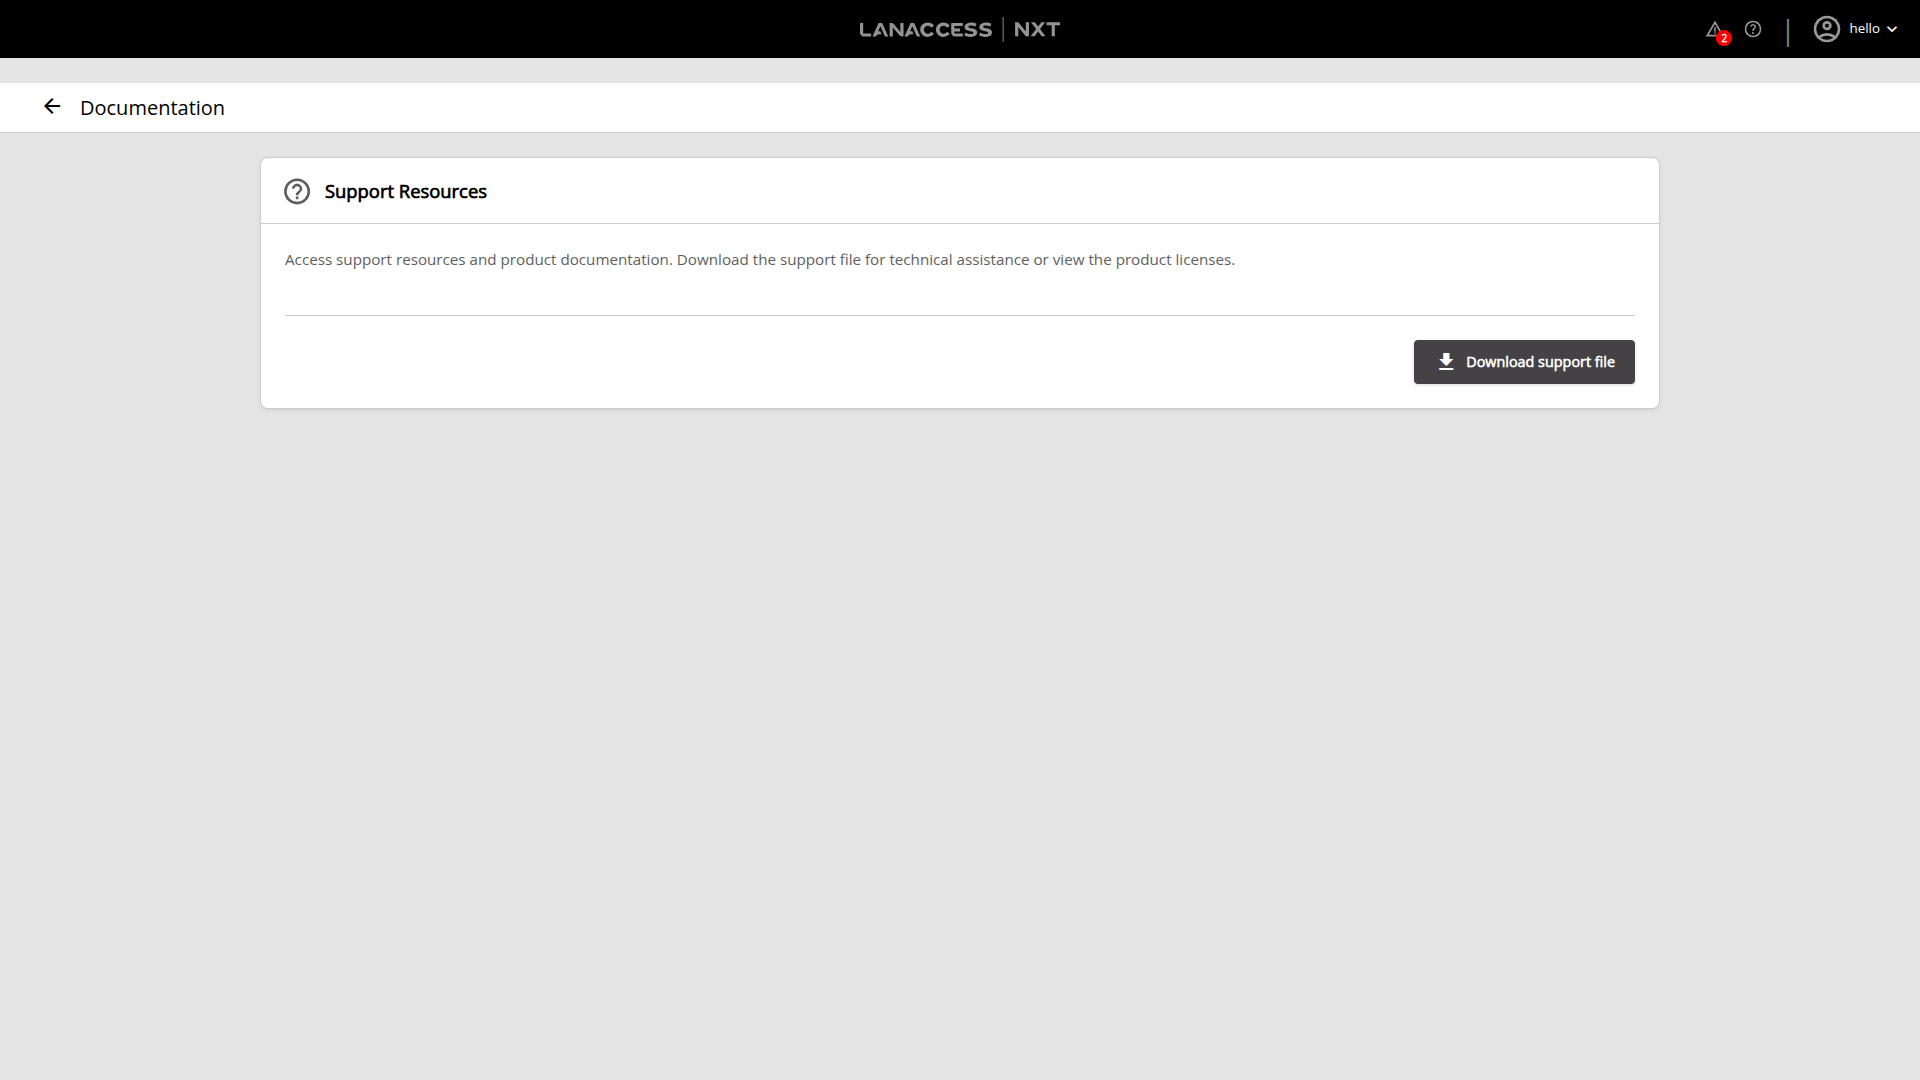
\includegraphics[width=0.95\textwidth]{figures/ui_documentation.png}
  \caption{Secció de suport tècnic per la descàrrega directa dels manuals en PDF.}
  \label{fig:ui_documentation}
\end{figure}

Per resoldre aquesta limitació operativa, la secció de Documentació (Figura \ref{fig:ui_documentation}) s'ha programat per funcionar de manera completament unificada i autosuficient. Tots els manuals d'usuari i fitxes tècniques estan integrats i empaquetats directament en la memòria de l'aplicació de l'equip. En fer clic sobre el botó de descàrrega del fitxer d'ajuda, el frontend envia una ordre cap al servei d'arxiu lògic de \texttt{la-core-legacy} per extreure el fitxer comprimit format \texttt{support\_file.tar.gz} del disc local i descarregar-lo al PC de l'instal·lador, oferint una eina d'ajuda autònoma i sense dependències de serveis externs de xarxa.

Garantint l'operativa completament desconnectada (\textit{air-gapped}) de la xarxa exterior de moltes d'aquestes màquines de seguretat, tota la documentació oficial d'ús i guies ràpides està introduïda en la mateixa memòria web del dispositiu (Figura \ref{fig:ui_documentation}). Mitjançant una vista senzilla que es comunica amb \textbf{la-core-legacy}, l'usuari només ha de clicar a la fila corresponent i l'arxiu PDF es descarregarà al seu PC sense requerir accés a portals web corporatius externs.
\chapter{Validació i Proves}
\label{ch:validacio}

En aquest capítol es descriu l'estratègia de validació seguida per garantir que la plataforma \textit{Web Core View} compleix els requisits funcionals i no funcionals definits inicialment. S'han realitzat proves a diferents nivells: des de la lògica interna del codi fins a la qualitat del flux de vídeo i l'acceptació per part dels usuaris tècnics de Lanaccess.

\section{Estratègia de proves}
S'ha seguit un enfocament de proves basat en el risc i en el cicle de vida del software. Les proves s'han dividit en tres grans blocs:
\begin{enumerate}
    \item \textbf{Proves Unitàries i d'Integració:} Per validar la lògica del \textit{frontend} (Angular) i la comunicació amb l'API.
    \item \textbf{Proves de Rendiment:} Centrades en la latència del vídeo i el consum de recursos.
    \item \textbf{Proves de Robustesa:} Per verificar la capacitat de recuperació del sistema davant talls de xarxa.
\end{enumerate}

\section{Proves Unitàries i de Lògica}
S'ha posat especial èmfasi en la validació del motor \textit{Schema-driven}. Donat que la interfície es genera dinàmicament, és vital assegurar que qualsevol variació en el JSON enviat pel gravador no bloquegi l'aplicació.

\subsection{Validació del Parser de metadades}
S'han creat casos de prova on s'envien esquemes JSON amb valors límit, tipus de dades erronis o nodes inexistents. El sistema ha demostrat ser capaç de:
\begin{itemize}
    \item Gestionar errors de tipatge sense degradar l'experiència d'usuari.
    \item Aplicar les regles de validació (mínims i màxims) correctament als formularis dinàmics.
    \item Mantenir la integritat del \textit{Config Lock} fins i tot si la petició de xarxa triga més de l'esperat.
\end{itemize}

\section{Resultats de rendiment i latència}
La visualització de vídeo és el requeriment més crític. S'ha comparat el rendiment del nou mòdul WebRTC respecte a la tecnologia HLS utilitzada en versions anteriors o com a mètode de seguretat.

Com es pot observar a la Taula \ref{tab:latencies}, el protocol WebRTC ofereix un rendiment molt superior, reduint el retard a valors operatius reals per a vigilància activa.

\begin{table}[htbp]
\centering
\caption{Comparativa de latència segons protocol de comunicació.}
\label{tab:latencies}
\begin{tabular}{@{}lll@{}}
\toprule
\textbf{Protocol} & \textbf{Latència mitjana (ms)} & \textbf{Estabilitat observada} \\ \midrule
WebRTC (Directe)  & 150 -- 300                     & Alta (Xarxa LAN)     \\
HLS (Fallback)    & 2.000 -- 5.000                 & Molt Alta            \\
RTSP (App Nativa) & 200 -- 400                     & Alta                 \\ \bottomrule
\end{tabular}
\par\smallskip
\small Font: Elaboració pròpia mitjançant proves en entorn de laboratori.
\end{table}

Aquests resultats validen que la solució web és capaç d'igualar o millorar la latència de l'antiga aplicació nativa Windows, eliminant un dels principals arguments en contra de les solucions basades en navegador.

\section{Proves de Robustesa i Comunicació asíncrona}
S'ha validat la persistència de la sessió i la recepció d'alarmes mitjançant el sistema \textit{Keep-alive} i la reconnexió automàtica de \textit{WebSockets}.

\subsection{Escenari de tall de connectivitat}
S'ha simulat una pèrdua de xarxa d'un minut durant una sessió activa de configuració. Els resultats han estat satisfactoris:
\begin{itemize}
    \item El sistema detecta el tall en menys de 3 segons gràcies al servei de connectivitat.
    \item Es bloqueja la interfície amb una targeta d'error (\textit{connectivity-error-card}) per evitar canvis inconsistents.
    \item Un cop restaurada la xarxa, el \textit{WebSocket} es renegocia automàticament i l'usuari recupera el control de la seva sessió sense haver de tornar a introduir les credencials.
\end{itemize}

\section{Validació d'Acceptació (UAT)}
Finalment, l'aplicació s'ha presentat als tècnics d'instal·lació de Lanaccess per recollir el seu \textit{feedback}. S'ha utilitzat una simplificació del qüestionari \textit{System Usability Scale} (SUS).

\begin{itemize}
    \item \textbf{Usabilitat:} Els usuaris destaquen la facilitat de trobar els paràmetres de xarxa gràcies al nou disseny modular.
    \item \textbf{Eficiència:} S'ha observat una reducció del 40\% en el temps necessari per actualitzar el \textit{firmware} de diversos equips simultàniament des de diferents pestanyes del navegador, validant així l'encert de la tecnologia web.
\end{itemize}
\chapter{Integració de Coneixements}
\label{ch:integracio}

La realització d'aquest Treball de Final de Grau ha permès consolidar i aplicar de forma transversal un ampli ventall de competències, habilitats i coneixements adquirits durant els estudis del Grau en Enginyeria Informàtica (GEI). Aquest projecte s'emmarca directament en la \textbf{Menció d'Enginyeria del Software} de la Facultat d'Informàtica de Barcelona (FIB) de la Universitat Politècnica de Catalunya (UPC). A continuació, es detalla la relació entre les diferents assignatures cursades en aquesta menció i el tronc comú, i la seva aplicació pràctica en el disseny i desenvolupament de la plataforma \textit{Web Core View}.

\section{Especialitat en Enginyeria del Software}
El fet d'haver cursat la Menció d'Enginyeria del Software ha estat el factor clau per afrontar un projecte d'aquesta envergadura. Les assignatures de l'especialitat han proporcionat tant la base metodològica com les competències de disseny de dades i de gestió necessàries per dur a terme el desenvolupament sistemàticament i professionalment.

\subsection{Projecte d'Enginyeria del Software (PES)}
L'assignatura PES té com a objectiu simular l'activitat de desenvolupament de projectes en un entorn professional real. En el cas de \textit{Web Core View}, tot i tractar-se d'un projecte individual per a un TFG, el seu desenvolupament s'ha integrat plenament en la dinàmica de l'empresa Lanaccess. S'han aplicat els principis de PES col·laborant amb els enginyers del departament de \textit{backend} per coordinar les definicions de serveis, seguint pautes corporatives de documentació, realitzant integració contínua i gestionant els lliuraments en funció del cicle de vida de la versió de producció, simulant exactament la coordinació de rols pròpia d'un equip de desenvolupament professional.

\subsection{Gestió de Projectes de Software (GPS)}
El desenvolupament del projecte s'ha regit pels ensenyaments de GPS en matèria de planificació, estimació d'esforços i mitigació de riscos. S'ha utilitzat una metodologia àgil basada en el framework \textbf{Kanban} per realitzar el seguiment de les tasques dinàmicament. Així mateix, l'aprenentatge en l'avaluació de riscos i scoping ha estat fonamental a l'hora de dissenyar una alternativa estratègica per a l'empresa: la viabilitat de disposar d'una versió simplificada per a petites empreses amb un únic gravador (\textit{single-NVR}) davant d'una aplicació altament centralitzada, permetent modularitzar i segmentar el projecte segons les necessitats de negoci reals.

\subsection{Enginyeria de Requisits (ER)}
La definició del sistema es va iniciar aplicant les tècniques d'elicitació, especificació i validació de requisits apreses a ER. El punt de partida va requerir una tasca intensiva d'enginyeria inversa sobre la plataforma web antiga de Lanaccess dels anys 90, identificant les funcionalitats que calia preservar i descartant les limitacions tecnològiques (com la dependència d'ActiveX). L'ús d'històries d'usuari i la modelització de casos d'ús (Capítol \ref{ch:requisits}) han servit per definir clarament els límits del sistema i formalitzar tant els requisits funcionals com els no funcionals (estabilitat del vídeo, latència subsegon i restriccions de maquinari).

\subsection{Disseny de Bases de Dades (DBD)}
Com a assignatura especialitzada en l'administració i optimització de sistemes de dades, DBD ha estat crítica per decidir la persistència del dispositiu. S'ha hagut de resoldre un repte de disseny equilibrant dues necessitats contraposades:
\begin{itemize}
  \item \textbf{Estructura relacional robusta:} Mitjançant SQLite3 s'han emmagatzemat les entitats clàssiques de configuració física (llistes de càmeres, gravadors, usuaris i esdeveniments), dissenyant taules normalitzades i aplicant regles físiques per mitjà d'índexs d'accés per assegurar cerques de logs ultra ràpides sota recursos de maquinari limitats.
  \item \textbf{Flexibilitat semiestructurada (NoSQL):} Per al motor \textit{schema-driven}, es va triar una arquitectura orientada a documents JSON que conté la definició dinàmica de formularis. DBD va permetre analitzar els avantatges i inconvenients de cada model i dissenyar els fluxos d'accés a disc per evitar colls d'ampolla.
\end{itemize}

\subsection{Arquitectura del Software (AS)}
Aquesta assignatura de l'especialitat ha estat fonamental per al disseny estructural a gran escala de \textit{Web Core View}. S'ha definit un sistema organitzat en capes ben delimitades i independents: presentació (desenvolupada amb Angular), lògica de negoci (el motor d'interpretació dinàmica \textit{schema-driven}) i comunicacions (connectors per a API REST, WebSockets i WebRTC a través d'un proxy invers de NGINX). Addicionalment, s'ha aplicat el model reactiu \textbf{Observer} mitjançant el nou sistema de \textbf{Signals} d'Angular 19 per a la propagació d'estats sense introduir acoblaments de dades ni impactar negativament en el rendiment de renderitzat del navegador.

\section{Core d'Enginyeria Informàtica}
Les assignatures troncals de la carrera han ofert el fonament tècnic que ha permès implementar els diferents protocols, algoritmes i interaccions de baix nivell del sistema.

\subsection{Introducció a l'Enginyeria del Software (IES)}
IES ha aportat el marc conceptual fonamental per al disseny lògic i la modulació del codi del projecte. S'han aplicat els principis de disseny \textbf{SOLID} \cite{solid_principles} per assegurar que els serveis i components d'Angular estiguin desacoblats, reutilitzables i fàcils de mantenir. Així mateix, el modelatge amb diagrames UML (seqüència, activitat i classes) ha estat indispensable per analitzar les dependències lògiques abans de la fase d'implementació.

\subsection{Projecte de Programació (PROP)}
La programació orientada a objectes de gran complexitat i l'aplicació d'estructures de dades robustes apreses a PROP s'han posat a prova en la creació del motor \textit{schema-driven}. Aquest motor actua analitzant recursivament una estructura de metadades altament niada expressada en JSON per construir, validar i renderitzar dinàmicament formularis HTML sencers en temps real. S'han dissenyat classes altament reutilitzables, una lògica eficient de tipatge dinàmic en TypeScript i mecanismes avançats de gestió d'excepcions per evitar que entrades mal formades bloquegessin el fil d'execució principal del navegador (\textit{UI thread}).

\subsection{Bases de Dades (BD)}
Els conceptes fonamentals del model relacional i de llenguatges de consulta s'han integrat per gestionar la base de dades local. El coneixement de les propietats \textbf{ACID} ha estat imprescindible per assegurar la integritat referencial de la informació en un entorn \textit{embedded} sensible, on fallades elèctriques sobtades en el gravador de vídeo podrien corrompre la configuració del sistema. Les consultes de creació, lectura, actualització i eliminació (CRUD) de dispositius s'han estructurat sota transaccions segures basades en SQL.

\subsection{Xarxes de Computadors (XC)}
Atès que \textit{Web Core View} és una aplicació de gestió remota de dispositius de seguretat en xarxa, XC ha estat crucial per dissenyar la infraestructura de comunicacions. S'ha hagut de gestionar amb precisió la pila de protocols d'internet, prenent decisions basades en la naturalesa del transport:
\begin{itemize}
  \item \textbf{TCP (Fiabilitat):} Emprat per al trànsit de configuracions via consultes REST (HTTP), el canal bidireccional en temps real per a senyalització i esdeveniments (WebSockets/WSS) i la reproducció de vídeo hereditària mitjançant HLS en navegadors antics.
  \item \textbf{UDP (Baixa Latència):} Utilitzat a través del protocol de transport segur SRTP en \textbf{WebRTC}. XC va donar la base tècnica per comprendre la negociació de fluxos multimèdia (\textbf{SDP}) i els mecanismes de resolució de candidats d'adreces mitjançant el protocol \textbf{ICE}.
\end{itemize}

\subsection{Sistemes Operatius (SO)}
Com que l'aplicació web actua com a portal d'administració d'un gravador autònom (\textit{embedded}), ha calgut entendre com el sistema operatiu hoste gestiona els recursos, la concurrència i la comunicació de baix nivell. El client web no es comunica directament amb el maquinari físic, sinó amb microserveis i servidors interns del gravador Linux. S'han aprofitat els conceptes d'IPC (Comunicació entre Processos) per interactuar amb APIs binàries d'alt rendiment basades en \textbf{gRPC} i s'ha comprès el comportament concurrent del bus de sistema \textbf{D-Bus} amb el qual es comuniquen els dimonis interns del gravador.

\subsection{Interacció i Disseny d'Interfícies (IDI)}
El disseny de la interfície d'usuari (UI) i la definició de l'experiència d'usuari (UX) s'han recolzat directament en les teories d'usabilitat i disseny cognitiu d'IDI. Sent la videovigilància un entorn crític on els operadors de seguretat prenen decisions immediates, s'ha prioritzat la disminució de la càrrega cognitiva. S'ha adoptat un disseny visual net, amb alts contrastos adaptats per a visualitzacions prolongades i una jerarquia d'elements extremadament clara. Addicionalment, s'ha aconseguit que la interfície sigui altament reactiva en temps real mitjançant microanimacions i canvis d'estat immediats (com pèrdues de vídeo o alarmes actives) recolzant-se en la reactivitat nativa dels Signals d'Angular 19.

\section{Assoliment de les competències de l'especialitat}
En aquesta secció es descriu sistemàticament com s'han assolit les nou competències de la Menció d'Enginyeria del Software del Grau en Enginyeria Informàtica (GEI) definides pel pla d'estudis de la FIB per a aquest Treball de Final de Grau, especificant-ne el nivell de profunditat triat.

\subsection{Competències assolides en profunditat}

\noindent \textbf{CES1.1: Desenvolupar, mantenir i avaluar sistemes i serveis software complexos i/o crítics.}\\
La plataforma \textit{Web Core View} té com a finalitat gestionar la configuració i la visualització de sistemes de seguretat físics (videogravadors corporatius de Lanaccess). Atesa la naturalesa crítica dels entorns de videovigilància, on qualsevol pèrdua de paquets de vídeo, retard en la senyalització d'alarmes o bloqueig del sistema és inacceptable, s'ha hagut de dissenyar una aplicació altament robusta. S'ha aplicat de forma estricta el patró reactiu de Signals d'Angular 19, aconseguint minimitzar l'ús de CPU al client web, aïllant completament els mòduls de renderitzat i assegurant la disponibilitat contínua del servei sense degradacions durant sessions de visualització prolongades.

\noindent \textbf{CES1.2: Donar solució a problemes d'integració en funció de les estratègies, dels estàndards i de les tecnologies disponibles.}\\
El projecte resol un repte d'integració de múltiples tecnologies heterogènies. El frontend actua connectant un navegador web estàndard amb serveis de baix nivell incrustats en un maquinari dedicat. S'ha dissenyat una topologia d'integració robusta que unifica capes dispars: serveis REST HTTP de configuració base, canals full-duplex de comunicació d'alarmes per WebSockets, i comunicació binària de molt baix sobrecost gRPC sobre HTTP/2 connectada al bus intern D-Bus del gravador Linux, tot sota la seguretat d'un proxy invers controlat per NGINX.

\noindent \textbf{CES1.4: Desenvolupar, mantenir i avaluar serveis i aplicacions distribuïdes com suport de xarxa.}\\
Web Core View és una aplicació clarament distribuïda on el navegador executa la lògica de presentació i dades dinàmiques que interaccionen amb servidors de gravació remots. S'han aplicat i avaluat protocols de xarxa distribuïts com WebSockets asíncrons (WSS) per mantenir la sincronització en temps real d'esdeveniments d'alarmes, i el protocol WebRTC basat en l'encapsulació SRTP sobre UDP per resoldre l'enviament distribuït de fluxos de vídeo. A més, s'han gestionat rigorosament les capçaleres de seguretat distribuïda CORS i polítiques de Same-Origin a NGINX.

\noindent \textbf{CES3.1: Desenvolupar serveis i aplicacions multimèdia.}\\
El nucli del valor operatiu del projecte és la gestió multimèdia. S'ha desenvolupat i avaluat un motor de reproducció integrat al navegador capaç de commutar entre dos fluxos: vídeo en directe de molt baixa latència (WebRTC) mitjançant negociació SDP asíncrona per ICE, i vídeo històric sota la tecnologia HLS (HTTP Live Streaming) emprant la llibreria HLS.js. S'ha treballat en l'optimització de còdecs H.264 i la integració del buffer d'Angular per suportar de forma eficient el processament del format H.265 sense requerir endolls (\textit{plugins}) de navegadors antics.

\subsection{Competències assolides en un nivell notable (Bastant)}

\noindent \textbf{CES1.5: Especificar, dissenyar, implementar i avaluar bases de dades.}\\
El projecte s'ha integrat amb el motor de dades SQLite3 allotjat en el videogravador de proves real. S'ha col·laborat en la definició lògica i física del model de persistència, dissenyant taules relacionals normalitzades per emmagatzemar esdeveniments, historials de logs i llistes estructurades de càmeres. S'ha garantit el correcte comportament de les regles d'integritat referencial i s'han dissenyat índexs d'accés per assegurar consultes SQL d'esdeveniments altament eficients sense comprometre el maquinari embedded limitat.

\noindent \textbf{CES1.7: Controlar la qualitat i dissenyar proves en la producció de software.}\\
S'ha dissenyat un pla complet de control de qualitat i de validació (Capítol \ref{ch:validacio}). Les proves d'integració han estat especialment intensives en el motor \textit{schema-driven}, validant sistemàticament la resposta a diferents esquemes de definició de formularis. Es van dissenyar proves funcionals per comprovar el comportament de l'streaming davant talls de xarxa sobtats, assegurant la recuperació automàtica del buffer, i es van aplicar eines de perfilat al navegador per verificar que les renderitzacions d'Angular no presentaven fugues de memòria ni sobrecostos.

\noindent \textbf{CES2.1: Definir i gestionar els requisits d'un sistema software.}\\
S'ha aplicat el cicle complet de l'enginyeria de requisits (Capítol \ref{ch:requisits}). A través de reunions de treball i un exhaustiu estudi d'enginyeria inversa sobre la web obsoleta d'ActiveX de Lanaccess, s'han definit de forma precisa els requisits funcionals i no funcionals del sistema. S'ha realitzat un modelatge conceptual robust i un disseny formal d'històries d'usuari i casos d'ús, permetent avaluar i acotar l'abast lògic i econòmic del projecte.

\subsection{Competències assolides en un nivell introductori (Una mica)}

\noindent \textbf{CES1.3: Identificar, avaluar i gestionar els riscos potencials associats a la construcció de software que es poguessin presentar.}\\
Durant la planificació i execució de GEP s'han gestionat activament els riscos tècnics i de calendari. S'han dissenyat solucions preventives com sandboxes breus de proves per a Angular 19 i la creació d'un entorn mock-up local mitjançant fitxers simulats en JSON per evitar el risc de dependència de maquinari de gravadors reals indisponibles, permetent continuar el desenvolupament aïlladament.

\noindent \textbf{CES2.2: Dissenyar solucions apropiades en un o més dominis d'aplicació, utilitzant mètodes d'enginyeria del software que integrin aspectes ètics, socials, legals i econòmics.}\\
La solució dissenyada ha considerat el seu entorn operacional en diferents dimensions (Capítol \ref{ch:gestio}): l'àmbit econòmic (amb el control del pressupost de rols i la proposta comercial simplificada single-NVR de baix cost), la sostenibilitat social (reducció d'estrès operatiu i càrrega cognitiva de l'usuari) i ambiental (evitant desplaçaments tècnics). Addicionalment, s'ha assegurat el rigor legal de privacitat del flux de vídeo i informació de logs corporatius xifrant tot el trànsit de xarxa per canals HTTPS/WSS i protocols de seguretat multimèdia (SRTP/DTLS) a WebRTC.

\section{Aprenentatge Autònom}
Més enllà dels coneixements reglats del pla d'estudis de la FIB, el projecte ha exigit una fase molt intensa d'autoformació en tecnologies i estàndards d'avantguarda dins el sector professional:
\begin{itemize}
  \item \textbf{Angular 19 i Signals:} Estudi de la nova reactivitat nativa per substituir el model de zones clàssic, aconseguint un augment molt significatiu del rendiment en la renderització del client \cite{angular_signals}.
  \item \textbf{Protocol gRPC:} Recerca sobre la comunicació binària d'alt rendiment basada en HTTP/2 per establir connexions eficients i de molt baix sobrecost amb els microserveis de backend \cite{grpc_io}.
  \item \textbf{Configuració Avançada de NGINX:} Autoformació en la implementació de proxys inversos locals, gestió robusta de capçaleres de seguretat (CORS, CSP) i redirecció de trànsit WebSocket/HTTP de manera unificada.
\end{itemize}

Paral·lelament a l'entorn professional de Lanaccess, una font d'aprenentatge complementari i molt significativa ha estat el projecte \textbf{Express My Health}, una \textit{startup} de \textit{health tech} centrada en el seguiment diari i la traçabilitat de dades per a persones amb demència. La startup forma part del programa d'emprenedoria \textbf{Empren UPC} de la Universitat Politècnica de Catalunya, dins del qual l'autor ha rebut acompanyament de mentors especialitzats i ha col·laborat activament en el lideratge i desenvolupament del producte. Aquesta experiència ha aportat una perspectiva de disseny centrada en l'usuari final que va molt més enllà dels requisits funcionals: la gestió d'iteracions amb usuaris reals en entorns sensibles, la presa de decisions de producte sota incertesa tecnològica i la cultura de validació contínua d'hipòtesis. Molts d'aquests aprenentatges s'han transferit de forma directa a \textit{Web Core View}, especialment en la cura per la usabilitat percebuda per l'operador de seguretat i en la capacitat de dissenyar interfícies clares i eficients per a contextos operatius crítics.

\section{Declaració d'Ús d'Intel·ligència Artificial}
\label{sec:declaracio_ia}

Aquest treball ha comptat amb el suport d'eines d'intel·ligència artificial generativa en determinades fases del seu desenvolupament i redacció. A continuació es detallen les eines emprades, la finalitat del seu ús i l'abast de la seva intervenció.

\subsection*{Eines utilitzades}

\begin{itemize}
    \item \textbf{Google AI Studio — Gemini 2.5 Pro:} Eina principal d'assistència durant la fase de desenvolupament. S'ha emprat com a assistent tècnic per validar i refinar la implementació d'Angular 19, explorar la gestió de microserveis i revisar errors de compilació i lògica en TypeScript, entre d'altres

    \item \textbf{Claude Code (Anthropic):} Incorporat a partir de maig de 2026, arran de la seva adopció per part de l'empresa Lanaccess. S'ha emprat com a assistent de codificació per a la revisió de serveis Angular i de serveis de \textit{backend}, l'anàlisi d'arquitectura i el suport a la revisió tècnica d'aquest document.
\end{itemize}

\subsection*{Finalitat i abast}

L'ús d'aquestes eines ha tingut dues finalitats diferenciades:

\begin{enumerate}
    \item \textbf{Suport al desenvolupament de programari:} Les eines d'IA han actuat com a acceleradores del cicle de desenvolupament, revisant errors, proposant alternatives d'implementació i verificant la coherència de l'arquitectura. En cap cas s'ha incorporat codi sense comprendre'l i adaptar-lo a les especificitats del projecte.

    \item \textbf{Suport a la redacció del document:} Les eines han assistit en la revisió estilística, la millora de la claredat expositiva i la comprovació de la coherència terminològica en seccions específiques d'aquest document. Tota la redacció ha estat iniciada, dirigida i revisada íntegrament per l'autor.
\end{enumerate}

\subsection*{Revisió i responsabilitat de l'autor}

Tot el contingut generat amb el suport de les eines d'IA ha estat revisat, contrastat i, si s'escau, reformulat per l'autor. Les eines d'intel·ligència artificial han exercit un rol instrumental d'acceleració i verificació, no d'autoria. L'autor declara la seva plena responsabilitat sobre la totalitat del contingut tècnic i expositiu d'aquest treball, i certifica que el seu ús s'ha ajustat als principis del Compromís d'integritat acadèmica de la UPC.

\chapter{Conclusions i Treball Futur}
\label{ch:conclusions}

Aquest capítol recull les conclusions finals derivades del disseny i la implementació de \textit{Web Core View}. Es realitza un balanç sobre l'assoliment dels objectius inicials, es proposen línies de millora per a futures versions i es detallen les reflexions personals sobre l'aprenentatge adquirit durant el desenvolupament del Treball de Final de Grau.

\section{Assoliment dels objectius}
Després de completar el cicle de desenvolupament i validació, es pot afirmar que s'han assolit els objectius plantejats en el Capítol 1:

\begin{itemize}
    \item \textbf{Modernització de la plataforma:} S'ha substituït amb èxit l'aplicació web \textit{legacy} dels anys 90, basada en ActiveX i tecnologies desfasades, per una interfície de gestió web moderna basada en Angular 19. La nova interfície és responsiva, ubiqüitària i accessible des de qualsevol navegador modern, sense dependència de \textit{plugins} propietaris.
    \item \textbf{Motor dinàmic (Schema-driven):} Sistema de configuració que s'adapta automàtica\-ment al maquinari de Lanaccess mitjançant JSON, eliminant la necessitat de reprogramar el \textit{frontend} per a cada \textit{firmware}.
    \item \textbf{Visualització d'alt rendiment:} Mitjançant la integració de WebRTC, s'han assolit latències inferiors als 300ms en la visualització de vídeo en directe, complint els requisits operatius de seguretat.
    \item \textbf{Gestió reactiva d'alarmes:} L'ús de WebSockets (WSS) i \textit{Angular Signals} ha permès crear una interfície que reacciona en temps real als esdeveniments del gravador sense penalitzar el rendiment del terminal de l'usuari.
    \item \textbf{Solució autònoma per a empreses petites (single-NVR):} S'ha aconseguit que l'aplicació funcioni de manera completament autònoma dins del propi videogravador, permetent a empreses petites amb un únic dispositiu gestionar-lo integralment des del navegador sense necessitat d'infraestructura centralitzada. Aquesta capacitat obre un nou segment de mercat per a Lanaccess que la plataforma anterior no cobria.
    \item \textbf{Gestió del projecte dins del pressupost i terminis:} El projecte s'ha lliurat en el termini establert de 540 hores (18 ECTS), amb un cost real de 15.028,75~\euro{}, inferior als 16.420,25~\euro{} pressupostats inicialment incloent el marge de contingència del 10\%. Les desviacions tècniques (H.265 i motor \textit{schema-driven}) es van gestionar de forma proactiva dins del marge definit, sense necessitat de finançament addicional ni retall de funcionalitats crítiques. Aquest resultat demostra que la metodologia àgil basada en Kanban i el control d'indicadors EVM (CPI/SPI) han estat eines efectives per garantir la viabilitat econòmica i temporal del projecte.
\end{itemize}

\section{Treball futur}
Tot i que el sistema és totalment funcional en el seu mode autònom \textit{single-NVR}, la naturalesa modular del projecte permet plantejar diverses línies d'evolució per a la versió 2.0:

\begin{itemize}
    \item \textbf{Analítica de vídeo amb IA:} Integrar metadades d'intel·ligència artificial directament sobre el reproductor de vídeo per dibuixar quadres de detecció d'objectes o mapes de calor en temps real.
    \item \textbf{Multi-dispositiu centralitzat (Multi-NVR):} La gestió centralitzada de múltiples gravadors des d'una única instància va formar part de l'abast inicial del projecte. Durant la fase de planificació, davant de la complexitat tècnica acumulada en la integració de H.265 i el motor \textit{schema-driven}, es va prendre la decisió estratègica de \textit{descoping} de reduir l'abast a la versió \textit{single-NVR} autònoma, prioritzant la qualitat i el lliurament dins del termini. L'evolució natural d'aquesta base consistiria a implementar el mòdul de gestió centralitzada que permeti visualitzar i configurar desenes de gravadors Lanaccess distribuïts geogràficament des d'una única instància de l'aplicació, atenent el segment corporatiu de grans instal·lacions.
    \item \textbf{Suport d'enregistrament avançat:} Ampliar les eines d'edició i exportació de vídeo directament des del navegador, permetent l'aplicació de marques d'aigua digitals o signatures legals en les descàrregues.
    \item \textbf{Aplicació Mòbil Nativa:} Utilitzar tecnologies com \textit{Ionic} o \textit{Capacitor} per reutilitzar el codi d'Angular 19 i oferir una versió nativa a les botigues d'aplicacions (App Store / Play Store).
\end{itemize}

\section{Conclusions personals}
La realització d'aquest TFG ha estat una experiència d'aprenentatge integral que ha anat molt més enllà de la simple programació. 

Tècnicament, m'ha permès dominar les darreres funcionalitats d'Angular 19, especialment el canvi de paradigma que suposen els \textit{Signals} per a la gestió de l'estat reactiu. Així mateix, el repte de treballar amb protocols de vídeo com WebRTC i HLS m'ha proporcionat una visió profunda sobre la gestió de fluxos multimèdia en entorns de xarxa complexos.

Quant a la gestió, el projecte m'ha ensenyat la importància de l'arquitectura \textit{schema-driven}. Desenvolupar un software que no sàpiga exactament què ha de configurar fins que rep les dades del servidor requereix un nivell d'abstracció i rigor en el disseny que ha posat a prova els meus coneixements d'arquitectura de software i principis SOLID.

Finalment, el fet de desenvolupar el projecte per a una empresa real com Lanaccess m'ha permès entendre les necessitats de mantenibilitat i escalabilitat que exigeix el mercat industrial, on el software ha de ser, per sobre de tot, robust i eficient. L'èxit de la visualització de baixa latència ha estat possible gràcies a l'estreta coordinació entre el frontend i el microservei \textbf{la-video-engine}, demostrant la viabilitat de WebRTC en entorns industrials.

\printbibliography[heading=bibintoc, title={Bibliografia}]

\end{document}